\documentclass[twoside]{book}

% Packages required by doxygen
\usepackage{calc}
\usepackage{doxygen}
\usepackage{graphicx}
\usepackage[utf8]{inputenc}
\usepackage{makeidx}
\usepackage{multicol}
\usepackage{multirow}
\usepackage{textcomp}
\usepackage[table]{xcolor}

% Font selection
\usepackage[T1]{fontenc}
\usepackage{mathptmx}
\usepackage[scaled=.90]{helvet}
\usepackage{courier}
\usepackage{amssymb}
\usepackage{sectsty}
\renewcommand{\familydefault}{\sfdefault}
\allsectionsfont{%
  \fontseries{bc}\selectfont%
  \color{darkgray}%
}
\renewcommand{\DoxyLabelFont}{%
  \fontseries{bc}\selectfont%
  \color{darkgray}%
}

% Page & text layout
\usepackage{geometry}
\geometry{%
  a4paper,%
  top=2.5cm,%
  bottom=2.5cm,%
  left=2.5cm,%
  right=2.5cm%
}
\tolerance=750
\hfuzz=15pt
\hbadness=750
\setlength{\emergencystretch}{15pt}
\setlength{\parindent}{0cm}
\setlength{\parskip}{0.2cm}
\makeatletter
\renewcommand{\paragraph}{%
  \@startsection{paragraph}{4}{0ex}{-1.0ex}{1.0ex}{%
    \normalfont\normalsize\bfseries\SS@parafont%
  }%
}
\renewcommand{\subparagraph}{%
  \@startsection{subparagraph}{5}{0ex}{-1.0ex}{1.0ex}{%
    \normalfont\normalsize\bfseries\SS@subparafont%
  }%
}
\makeatother

% Headers & footers
\usepackage{fancyhdr}
\pagestyle{fancyplain}
\fancyhead[LE]{\fancyplain{}{\bfseries\thepage}}
\fancyhead[CE]{\fancyplain{}{}}
\fancyhead[RE]{\fancyplain{}{\bfseries\leftmark}}
\fancyhead[LO]{\fancyplain{}{\bfseries\rightmark}}
\fancyhead[CO]{\fancyplain{}{}}
\fancyhead[RO]{\fancyplain{}{\bfseries\thepage}}
\fancyfoot[LE]{\fancyplain{}{}}
\fancyfoot[CE]{\fancyplain{}{}}
\fancyfoot[RE]{\fancyplain{}{\bfseries\scriptsize Generated on Sat Oct 19 2013 20\-:21\-:53 for zebra-\/zmachine-\/interpreter by Doxygen }}
\fancyfoot[LO]{\fancyplain{}{\bfseries\scriptsize Generated on Sat Oct 19 2013 20\-:21\-:53 for zebra-\/zmachine-\/interpreter by Doxygen }}
\fancyfoot[CO]{\fancyplain{}{}}
\fancyfoot[RO]{\fancyplain{}{}}
\renewcommand{\footrulewidth}{0.4pt}
\renewcommand{\chaptermark}[1]{%
  \markboth{#1}{}%
}
\renewcommand{\sectionmark}[1]{%
  \markright{\thesection\ #1}%
}

% Indices & bibliography
\usepackage{natbib}
\usepackage[titles]{tocloft}
\setcounter{tocdepth}{3}
\setcounter{secnumdepth}{5}
\makeindex

% Hyperlinks (required, but should be loaded last)
\usepackage{ifpdf}
\ifpdf
  \usepackage[pdftex,pagebackref=true]{hyperref}
\else
  \usepackage[ps2pdf,pagebackref=true]{hyperref}
\fi
\hypersetup{%
  colorlinks=true,%
  linkcolor=blue,%
  citecolor=blue,%
  unicode%
}

% Custom commands
\newcommand{\clearemptydoublepage}{%
  \newpage{\pagestyle{empty}\cleardoublepage}%
}


%===== C O N T E N T S =====

\begin{document}

% Titlepage & ToC
\hypersetup{pageanchor=false}
\pagenumbering{roman}
\begin{titlepage}
\vspace*{7cm}
\begin{center}%
{\Large zebra-\/zmachine-\/interpreter }\\
\vspace*{1cm}
{\large Generated by Doxygen 1.8.5}\\
\vspace*{0.5cm}
{\small Sat Oct 19 2013 20:21:53}\\
\end{center}
\end{titlepage}
\clearemptydoublepage
\tableofcontents
\clearemptydoublepage
\pagenumbering{arabic}
\hypersetup{pageanchor=true}

%--- Begin generated contents ---
\chapter{Hierarchical Index}
\section{Class Hierarchy}
This inheritance list is sorted roughly, but not completely, alphabetically\-:\begin{DoxyCompactList}
\item exception\begin{DoxyCompactList}
\item \contentsline{section}{Illegal\-Dictionary\-Index}{\pageref{class_illegal_dictionary_index}}{}
\item \contentsline{section}{Illegal\-Object\-Index}{\pageref{class_illegal_object_index}}{}
\item \contentsline{section}{Illegal\-Property\-Index}{\pageref{class_illegal_property_index}}{}
\item \contentsline{section}{Illegal\-Z\-Char\-Exception}{\pageref{class_illegal_z_char_exception}}{}
\item \contentsline{section}{Illegal\-Z\-Char\-String}{\pageref{class_illegal_z_char_string}}{}
\item \contentsline{section}{Stack\-Empty\-Exception}{\pageref{class_stack_empty_exception}}{}
\item \contentsline{section}{Stack\-Full\-Exception}{\pageref{class_stack_full_exception}}{}
\item \contentsline{section}{Z\-Memory\-Read\-Out\-Of\-Bounds}{\pageref{class_z_memory_read_out_of_bounds}}{}
\item \contentsline{section}{Z\-Memory\-Write\-Out\-Of\-Bounds}{\pageref{class_z_memory_write_out_of_bounds}}{}
\end{DoxyCompactList}
\item \contentsline{section}{Object\-Property}{\pageref{struct_object_property}}{}
\item \contentsline{section}{z\-Char\-Stringto\-Z\-S\-C\-I\-I\-Helper\-\_\-save\-State}{\pageref{structz_char_stringto_z_s_c_i_i_helper__save_state}}{}
\item \contentsline{section}{Z\-Dictionary}{\pageref{class_z_dictionary}}{}
\item \contentsline{section}{z\-Dictionary\-Word}{\pageref{structz_dictionary_word}}{}
\item \contentsline{section}{Z\-Error}{\pageref{class_z_error}}{}
\item \contentsline{section}{Z\-Memory}{\pageref{class_z_memory}}{}
\item \contentsline{section}{Z\-Object\-Table}{\pageref{class_z_object_table}}{}
\item \contentsline{section}{Z\-Stack}{\pageref{class_z_stack}}{}
\end{DoxyCompactList}

\chapter{Class Index}
\section{Class List}
Here are the classes, structs, unions and interfaces with brief descriptions\-:\begin{DoxyCompactList}
\item\contentsline{section}{\hyperlink{class_illegal_dictionary_index}{Illegal\-Dictionary\-Index} }{\pageref{class_illegal_dictionary_index}}{}
\item\contentsline{section}{\hyperlink{class_illegal_object_index}{Illegal\-Object\-Index} }{\pageref{class_illegal_object_index}}{}
\item\contentsline{section}{\hyperlink{class_illegal_property_index}{Illegal\-Property\-Index} }{\pageref{class_illegal_property_index}}{}
\item\contentsline{section}{\hyperlink{class_illegal_z_char_exception}{Illegal\-Z\-Char\-Exception} }{\pageref{class_illegal_z_char_exception}}{}
\item\contentsline{section}{\hyperlink{class_illegal_z_char_string}{Illegal\-Z\-Char\-String} }{\pageref{class_illegal_z_char_string}}{}
\item\contentsline{section}{\hyperlink{struct_object_property}{Object\-Property} }{\pageref{struct_object_property}}{}
\item\contentsline{section}{\hyperlink{class_stack_empty_exception}{Stack\-Empty\-Exception} }{\pageref{class_stack_empty_exception}}{}
\item\contentsline{section}{\hyperlink{class_stack_full_exception}{Stack\-Full\-Exception} }{\pageref{class_stack_full_exception}}{}
\item\contentsline{section}{\hyperlink{structz_char_stringto_z_s_c_i_i_helper__save_state}{z\-Char\-Stringto\-Z\-S\-C\-I\-I\-Helper\-\_\-save\-State} }{\pageref{structz_char_stringto_z_s_c_i_i_helper__save_state}}{}
\item\contentsline{section}{\hyperlink{class_z_dictionary}{Z\-Dictionary} }{\pageref{class_z_dictionary}}{}
\item\contentsline{section}{\hyperlink{structz_dictionary_word}{z\-Dictionary\-Word} }{\pageref{structz_dictionary_word}}{}
\item\contentsline{section}{\hyperlink{class_z_error}{Z\-Error} }{\pageref{class_z_error}}{}
\item\contentsline{section}{\hyperlink{class_z_memory}{Z\-Memory} }{\pageref{class_z_memory}}{}
\item\contentsline{section}{\hyperlink{class_z_memory_read_out_of_bounds}{Z\-Memory\-Read\-Out\-Of\-Bounds} }{\pageref{class_z_memory_read_out_of_bounds}}{}
\item\contentsline{section}{\hyperlink{class_z_memory_write_out_of_bounds}{Z\-Memory\-Write\-Out\-Of\-Bounds} }{\pageref{class_z_memory_write_out_of_bounds}}{}
\item\contentsline{section}{\hyperlink{class_z_object_table}{Z\-Object\-Table} }{\pageref{class_z_object_table}}{}
\item\contentsline{section}{\hyperlink{class_z_stack}{Z\-Stack} }{\pageref{class_z_stack}}{}
\end{DoxyCompactList}

\chapter{File Index}
\section{File List}
Here is a list of all files with brief descriptions\-:\begin{DoxyCompactList}
\item\contentsline{section}{H\-:/code/c++/zebra-\/zmachine-\/interpreter/zdictionary/zdictionary/\hyperlink{zdictionary_2zdictionary_2main_8cpp}{main.\-cpp} }{\pageref{zdictionary_2zdictionary_2main_8cpp}}{}
\item\contentsline{section}{H\-:/code/c++/zebra-\/zmachine-\/interpreter/zdictionary/zdictionary/\hyperlink{zdictionary_8cpp}{zdictionary.\-cpp} }{\pageref{zdictionary_8cpp}}{}
\item\contentsline{section}{H\-:/code/c++/zebra-\/zmachine-\/interpreter/zdictionary/zdictionary/\hyperlink{zdictionary_8h}{zdictionary.\-h} }{\pageref{zdictionary_8h}}{}
\item\contentsline{section}{H\-:/code/c++/zebra-\/zmachine-\/interpreter/zerror/zerror/\hyperlink{zerror_2zerror_2main_8cpp}{main.\-cpp} }{\pageref{zerror_2zerror_2main_8cpp}}{}
\item\contentsline{section}{H\-:/code/c++/zebra-\/zmachine-\/interpreter/zerror/zerror/\hyperlink{zerror_8cpp}{zerror.\-cpp} }{\pageref{zerror_8cpp}}{}
\item\contentsline{section}{H\-:/code/c++/zebra-\/zmachine-\/interpreter/zerror/zerror/\hyperlink{zerror_8h}{zerror.\-h} }{\pageref{zerror_8h}}{}
\item\contentsline{section}{H\-:/code/c++/zebra-\/zmachine-\/interpreter/zglobal/\hyperlink{zglobal_8cpp}{zglobal.\-cpp} }{\pageref{zglobal_8cpp}}{}
\item\contentsline{section}{H\-:/code/c++/zebra-\/zmachine-\/interpreter/zglobal/\hyperlink{zglobal_8h}{zglobal.\-h} }{\pageref{zglobal_8h}}{}
\item\contentsline{section}{H\-:/code/c++/zebra-\/zmachine-\/interpreter/zmemory/zmemory/\hyperlink{zmemory_2zmemory_2main_8cpp}{main.\-cpp} }{\pageref{zmemory_2zmemory_2main_8cpp}}{}
\item\contentsline{section}{H\-:/code/c++/zebra-\/zmachine-\/interpreter/zmemory/zmemory/\hyperlink{zmemory_8cpp}{zmemory.\-cpp} }{\pageref{zmemory_8cpp}}{}
\item\contentsline{section}{H\-:/code/c++/zebra-\/zmachine-\/interpreter/zmemory/zmemory/\hyperlink{zmemory_8h}{zmemory.\-h} }{\pageref{zmemory_8h}}{}
\item\contentsline{section}{H\-:/code/c++/zebra-\/zmachine-\/interpreter/zmemory/zmemory/\hyperlink{zobject_8cpp}{zobject.\-cpp} }{\pageref{zobject_8cpp}}{}
\item\contentsline{section}{H\-:/code/c++/zebra-\/zmachine-\/interpreter/zmemory/zmemory/\hyperlink{zobject_8h}{zobject.\-h} }{\pageref{zobject_8h}}{}
\item\contentsline{section}{H\-:/code/c++/zebra-\/zmachine-\/interpreter/zstack/zstack/\hyperlink{zstack_2zstack_2main_8cpp}{main.\-cpp} }{\pageref{zstack_2zstack_2main_8cpp}}{}
\item\contentsline{section}{H\-:/code/c++/zebra-\/zmachine-\/interpreter/zstack/zstack/\hyperlink{zstack_8cpp}{zstack.\-cpp} }{\pageref{zstack_8cpp}}{}
\item\contentsline{section}{H\-:/code/c++/zebra-\/zmachine-\/interpreter/zstack/zstack/\hyperlink{zstack_8h}{zstack.\-h} }{\pageref{zstack_8h}}{}
\item\contentsline{section}{H\-:/code/c++/zebra-\/zmachine-\/interpreter/ztext/ztext/\hyperlink{ztext_2ztext_2main_8cpp}{main.\-cpp} }{\pageref{ztext_2ztext_2main_8cpp}}{}
\item\contentsline{section}{H\-:/code/c++/zebra-\/zmachine-\/interpreter/ztext/ztext/\hyperlink{ztext_8cpp}{ztext.\-cpp} }{\pageref{ztext_8cpp}}{}
\item\contentsline{section}{H\-:/code/c++/zebra-\/zmachine-\/interpreter/ztext/ztext/\hyperlink{ztext_8h}{ztext.\-h} }{\pageref{ztext_8h}}{}
\end{DoxyCompactList}

\chapter{Class Documentation}
\hypertarget{class_illegal_dictionary_index}{\section{Illegal\-Dictionary\-Index Class Reference}
\label{class_illegal_dictionary_index}\index{Illegal\-Dictionary\-Index@{Illegal\-Dictionary\-Index}}
}


{\ttfamily \#include $<$zdictionary.\-h$>$}

Inheritance diagram for Illegal\-Dictionary\-Index\-:\begin{figure}[H]
\begin{center}
\leavevmode
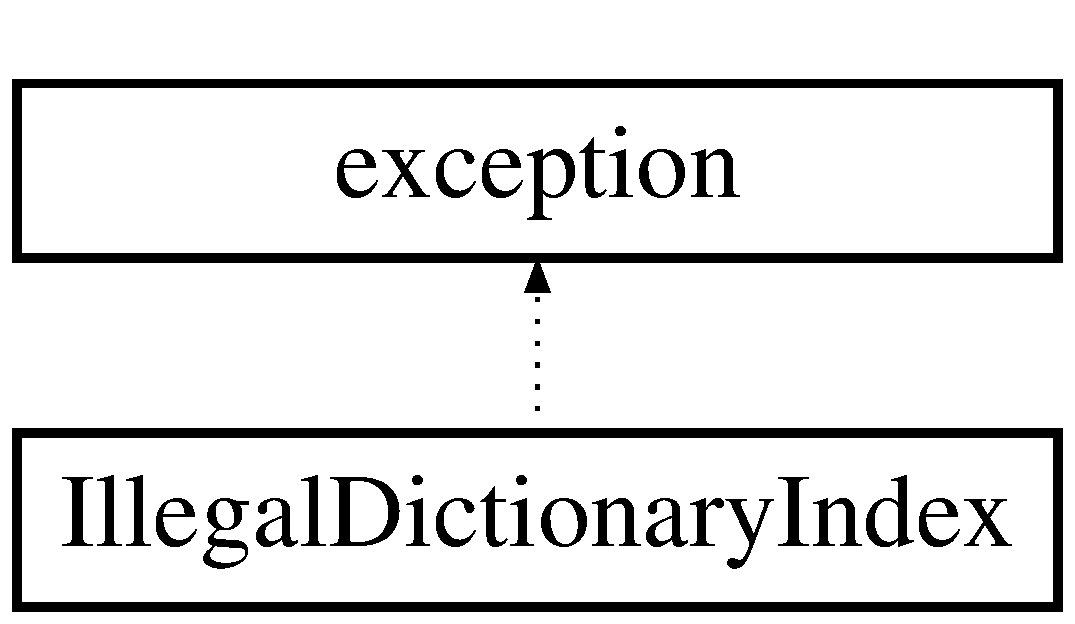
\includegraphics[height=2.000000cm]{class_illegal_dictionary_index}
\end{center}
\end{figure}
\subsection*{Public Member Functions}
\begin{DoxyCompactItemize}
\item 
\hyperlink{class_illegal_dictionary_index_a9303545239c0140b2f6f251002e10c19}{Illegal\-Dictionary\-Index} ()
\end{DoxyCompactItemize}


\subsection{Constructor \& Destructor Documentation}
\hypertarget{class_illegal_dictionary_index_a9303545239c0140b2f6f251002e10c19}{\index{Illegal\-Dictionary\-Index@{Illegal\-Dictionary\-Index}!Illegal\-Dictionary\-Index@{Illegal\-Dictionary\-Index}}
\index{Illegal\-Dictionary\-Index@{Illegal\-Dictionary\-Index}!IllegalDictionaryIndex@{Illegal\-Dictionary\-Index}}
\subsubsection[{Illegal\-Dictionary\-Index}]{\setlength{\rightskip}{0pt plus 5cm}Illegal\-Dictionary\-Index\-::\-Illegal\-Dictionary\-Index (
\begin{DoxyParamCaption}
{}
\end{DoxyParamCaption}
)\hspace{0.3cm}{\ttfamily [inline]}}}\label{class_illegal_dictionary_index_a9303545239c0140b2f6f251002e10c19}


The documentation for this class was generated from the following file\-:\begin{DoxyCompactItemize}
\item 
H\-:/code/c++/zebra-\/zmachine-\/interpreter/zdictionary/zdictionary/\hyperlink{zdictionary_8h}{zdictionary.\-h}\end{DoxyCompactItemize}

\hypertarget{class_illegal_object_index}{\section{Illegal\-Object\-Index Class Reference}
\label{class_illegal_object_index}\index{Illegal\-Object\-Index@{Illegal\-Object\-Index}}
}


{\ttfamily \#include $<$zobject.\-h$>$}

Inheritance diagram for Illegal\-Object\-Index\-:\begin{figure}[H]
\begin{center}
\leavevmode
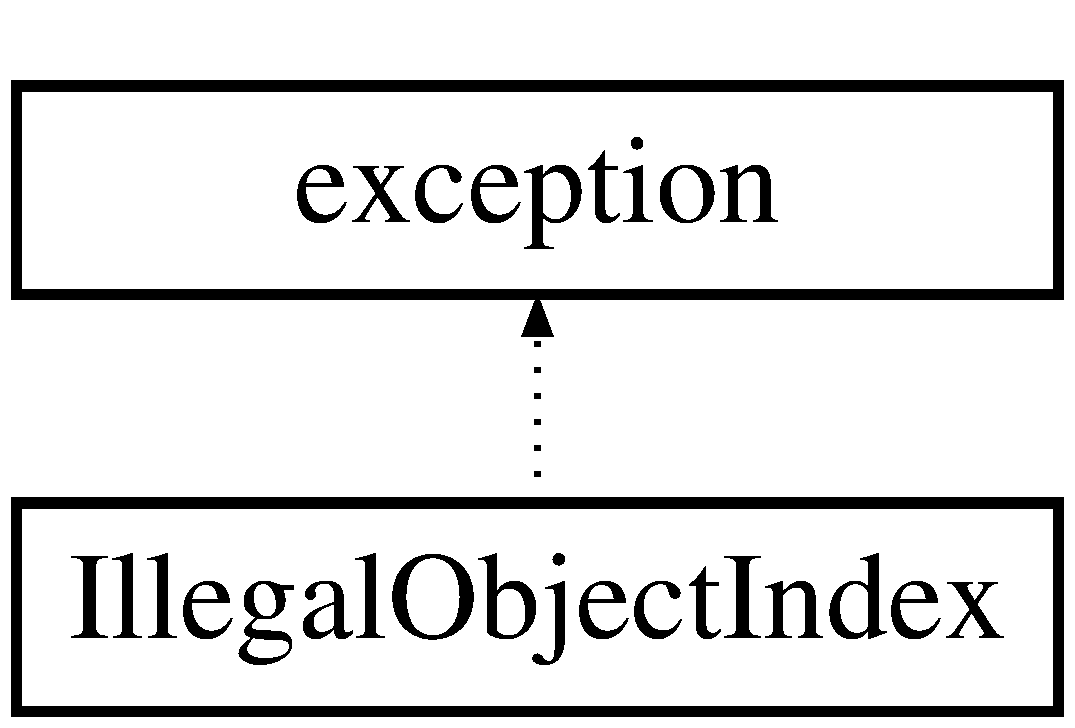
\includegraphics[height=2.000000cm]{class_illegal_object_index}
\end{center}
\end{figure}
\subsection*{Public Member Functions}
\begin{DoxyCompactItemize}
\item 
\hyperlink{class_illegal_object_index_a2a3fec4c49b994784797db8019b501d0}{Illegal\-Object\-Index} ()
\end{DoxyCompactItemize}


\subsection{Constructor \& Destructor Documentation}
\hypertarget{class_illegal_object_index_a2a3fec4c49b994784797db8019b501d0}{\index{Illegal\-Object\-Index@{Illegal\-Object\-Index}!Illegal\-Object\-Index@{Illegal\-Object\-Index}}
\index{Illegal\-Object\-Index@{Illegal\-Object\-Index}!IllegalObjectIndex@{Illegal\-Object\-Index}}
\subsubsection[{Illegal\-Object\-Index}]{\setlength{\rightskip}{0pt plus 5cm}Illegal\-Object\-Index\-::\-Illegal\-Object\-Index (
\begin{DoxyParamCaption}
{}
\end{DoxyParamCaption}
)\hspace{0.3cm}{\ttfamily [inline]}}}\label{class_illegal_object_index_a2a3fec4c49b994784797db8019b501d0}


The documentation for this class was generated from the following file\-:\begin{DoxyCompactItemize}
\item 
H\-:/code/c++/zebra-\/zmachine-\/interpreter/zmemory/zmemory/\hyperlink{zobject_8h}{zobject.\-h}\end{DoxyCompactItemize}

\hypertarget{class_illegal_property_index}{\section{Illegal\-Property\-Index Class Reference}
\label{class_illegal_property_index}\index{Illegal\-Property\-Index@{Illegal\-Property\-Index}}
}


{\ttfamily \#include $<$zobject.\-h$>$}

Inheritance diagram for Illegal\-Property\-Index\-:\begin{figure}[H]
\begin{center}
\leavevmode
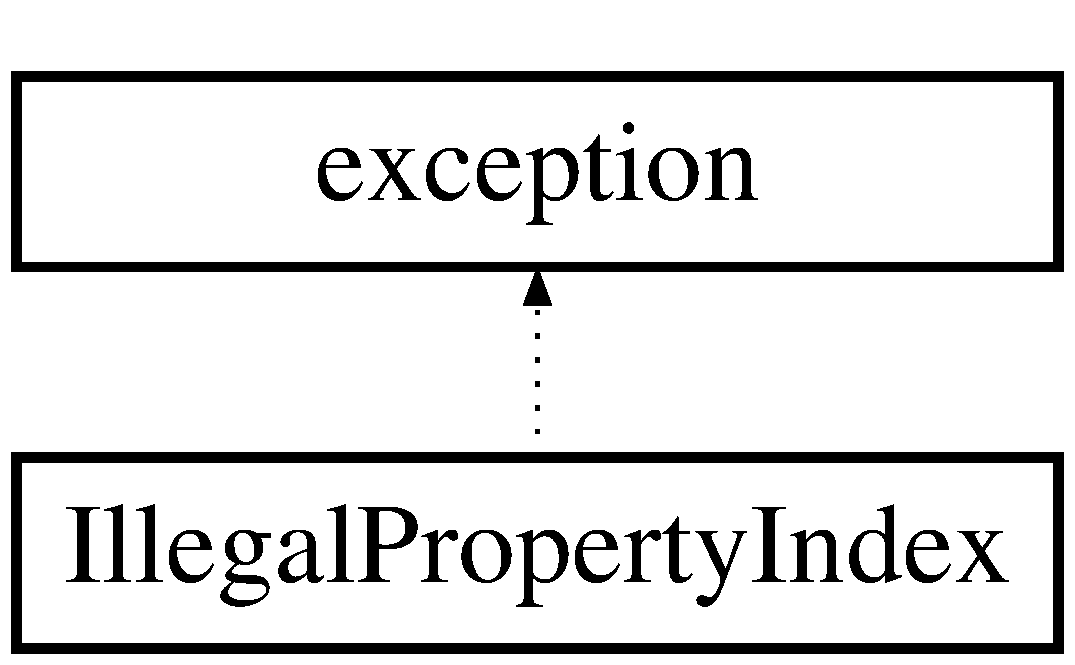
\includegraphics[height=2.000000cm]{class_illegal_property_index}
\end{center}
\end{figure}
\subsection*{Public Member Functions}
\begin{DoxyCompactItemize}
\item 
\hyperlink{class_illegal_property_index_a8ec7160a105d9feb5197d71d03126df9}{Illegal\-Property\-Index} ()
\end{DoxyCompactItemize}


\subsection{Constructor \& Destructor Documentation}
\hypertarget{class_illegal_property_index_a8ec7160a105d9feb5197d71d03126df9}{\index{Illegal\-Property\-Index@{Illegal\-Property\-Index}!Illegal\-Property\-Index@{Illegal\-Property\-Index}}
\index{Illegal\-Property\-Index@{Illegal\-Property\-Index}!IllegalPropertyIndex@{Illegal\-Property\-Index}}
\subsubsection[{Illegal\-Property\-Index}]{\setlength{\rightskip}{0pt plus 5cm}Illegal\-Property\-Index\-::\-Illegal\-Property\-Index (
\begin{DoxyParamCaption}
{}
\end{DoxyParamCaption}
)\hspace{0.3cm}{\ttfamily [inline]}}}\label{class_illegal_property_index_a8ec7160a105d9feb5197d71d03126df9}


The documentation for this class was generated from the following file\-:\begin{DoxyCompactItemize}
\item 
H\-:/code/c++/zebra-\/zmachine-\/interpreter/zmemory/zmemory/\hyperlink{zobject_8h}{zobject.\-h}\end{DoxyCompactItemize}

\hypertarget{class_illegal_z_char_exception}{\section{Illegal\-Z\-Char\-Exception Class Reference}
\label{class_illegal_z_char_exception}\index{Illegal\-Z\-Char\-Exception@{Illegal\-Z\-Char\-Exception}}
}


{\ttfamily \#include $<$ztext.\-h$>$}

Inheritance diagram for Illegal\-Z\-Char\-Exception\-:\begin{figure}[H]
\begin{center}
\leavevmode
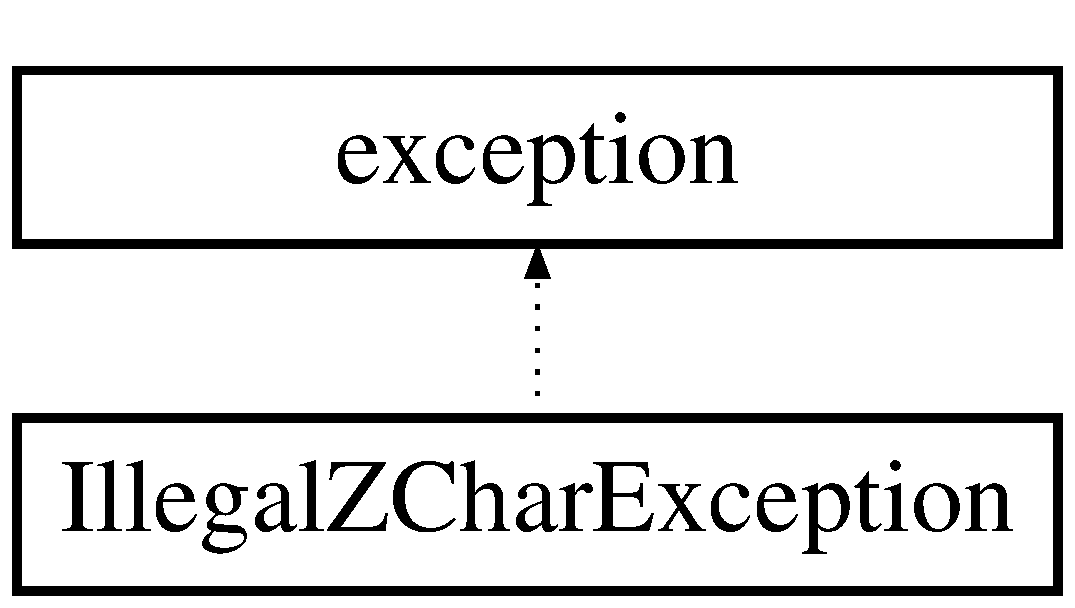
\includegraphics[height=2.000000cm]{class_illegal_z_char_exception}
\end{center}
\end{figure}
\subsection*{Public Member Functions}
\begin{DoxyCompactItemize}
\item 
\hyperlink{class_illegal_z_char_exception_a0275d787d4a0658695d422471e18ea55}{Illegal\-Z\-Char\-Exception} ()
\end{DoxyCompactItemize}


\subsection{Constructor \& Destructor Documentation}
\hypertarget{class_illegal_z_char_exception_a0275d787d4a0658695d422471e18ea55}{\index{Illegal\-Z\-Char\-Exception@{Illegal\-Z\-Char\-Exception}!Illegal\-Z\-Char\-Exception@{Illegal\-Z\-Char\-Exception}}
\index{Illegal\-Z\-Char\-Exception@{Illegal\-Z\-Char\-Exception}!IllegalZCharException@{Illegal\-Z\-Char\-Exception}}
\subsubsection[{Illegal\-Z\-Char\-Exception}]{\setlength{\rightskip}{0pt plus 5cm}Illegal\-Z\-Char\-Exception\-::\-Illegal\-Z\-Char\-Exception (
\begin{DoxyParamCaption}
{}
\end{DoxyParamCaption}
)\hspace{0.3cm}{\ttfamily [inline]}}}\label{class_illegal_z_char_exception_a0275d787d4a0658695d422471e18ea55}


The documentation for this class was generated from the following file\-:\begin{DoxyCompactItemize}
\item 
H\-:/code/c++/zebra-\/zmachine-\/interpreter/ztext/ztext/\hyperlink{ztext_8h}{ztext.\-h}\end{DoxyCompactItemize}

\hypertarget{class_illegal_z_char_string}{\section{Illegal\-Z\-Char\-String Class Reference}
\label{class_illegal_z_char_string}\index{Illegal\-Z\-Char\-String@{Illegal\-Z\-Char\-String}}
}


{\ttfamily \#include $<$ztext.\-h$>$}

Inheritance diagram for Illegal\-Z\-Char\-String\-:\begin{figure}[H]
\begin{center}
\leavevmode
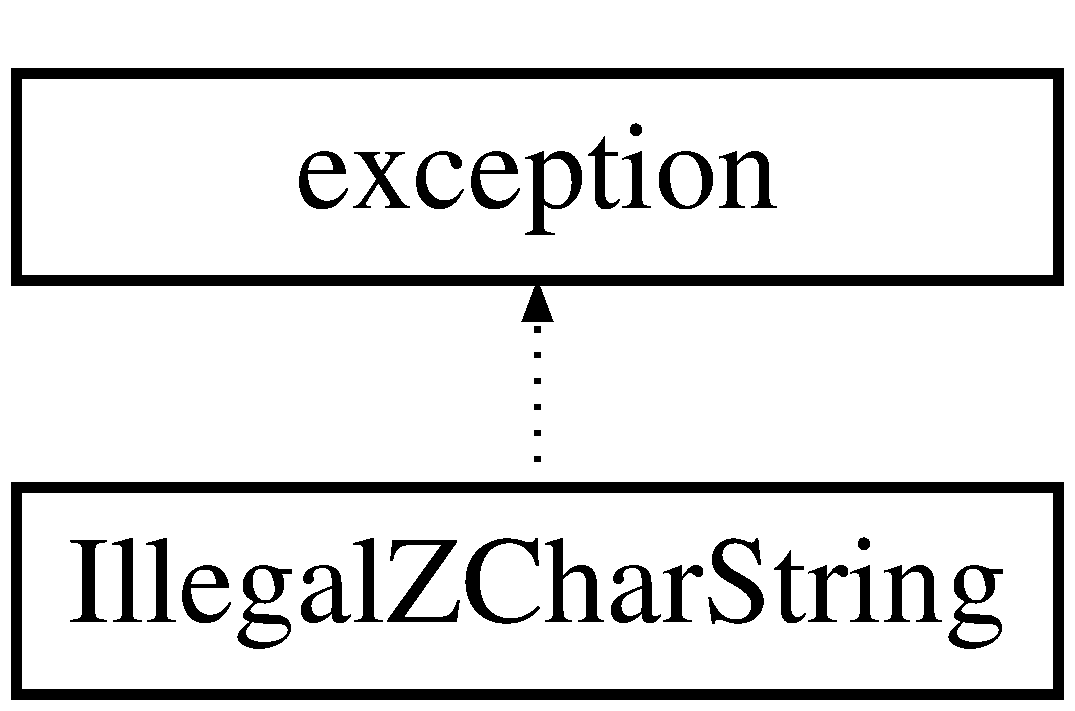
\includegraphics[height=2.000000cm]{class_illegal_z_char_string}
\end{center}
\end{figure}
\subsection*{Public Member Functions}
\begin{DoxyCompactItemize}
\item 
\hyperlink{class_illegal_z_char_string_a3fd1ed7a5a9a8cf2c5d81292df53b970}{Illegal\-Z\-Char\-String} ()
\end{DoxyCompactItemize}


\subsection{Constructor \& Destructor Documentation}
\hypertarget{class_illegal_z_char_string_a3fd1ed7a5a9a8cf2c5d81292df53b970}{\index{Illegal\-Z\-Char\-String@{Illegal\-Z\-Char\-String}!Illegal\-Z\-Char\-String@{Illegal\-Z\-Char\-String}}
\index{Illegal\-Z\-Char\-String@{Illegal\-Z\-Char\-String}!IllegalZCharString@{Illegal\-Z\-Char\-String}}
\subsubsection[{Illegal\-Z\-Char\-String}]{\setlength{\rightskip}{0pt plus 5cm}Illegal\-Z\-Char\-String\-::\-Illegal\-Z\-Char\-String (
\begin{DoxyParamCaption}
{}
\end{DoxyParamCaption}
)\hspace{0.3cm}{\ttfamily [inline]}}}\label{class_illegal_z_char_string_a3fd1ed7a5a9a8cf2c5d81292df53b970}


The documentation for this class was generated from the following file\-:\begin{DoxyCompactItemize}
\item 
H\-:/code/c++/zebra-\/zmachine-\/interpreter/ztext/ztext/\hyperlink{ztext_8h}{ztext.\-h}\end{DoxyCompactItemize}

\hypertarget{struct_object_property}{\section{Object\-Property Struct Reference}
\label{struct_object_property}\index{Object\-Property@{Object\-Property}}
}


{\ttfamily \#include $<$zobject.\-h$>$}

\subsection*{Public Attributes}
\begin{DoxyCompactItemize}
\item 
\hyperlink{zglobal_8h_a6507dc55d18847442d5fb20b6c73fe73}{zword} \hyperlink{struct_object_property_a3f25a7e52c3cfe6f23dd06f7f8f9099d}{property\-Data\-Addr}
\item 
\hyperlink{zglobal_8h_a718b4eb2652c286f4d42dc18a8e71a1a}{ulong} \hyperlink{struct_object_property_ab1405932da7aee1f5de0b906a9020f78}{property\-Data\-Size}
\end{DoxyCompactItemize}


\subsection{Member Data Documentation}
\hypertarget{struct_object_property_a3f25a7e52c3cfe6f23dd06f7f8f9099d}{\index{Object\-Property@{Object\-Property}!property\-Data\-Addr@{property\-Data\-Addr}}
\index{property\-Data\-Addr@{property\-Data\-Addr}!ObjectProperty@{Object\-Property}}
\subsubsection[{property\-Data\-Addr}]{\setlength{\rightskip}{0pt plus 5cm}{\bf zword} Object\-Property\-::property\-Data\-Addr}}\label{struct_object_property_a3f25a7e52c3cfe6f23dd06f7f8f9099d}
\hypertarget{struct_object_property_ab1405932da7aee1f5de0b906a9020f78}{\index{Object\-Property@{Object\-Property}!property\-Data\-Size@{property\-Data\-Size}}
\index{property\-Data\-Size@{property\-Data\-Size}!ObjectProperty@{Object\-Property}}
\subsubsection[{property\-Data\-Size}]{\setlength{\rightskip}{0pt plus 5cm}{\bf ulong} Object\-Property\-::property\-Data\-Size}}\label{struct_object_property_ab1405932da7aee1f5de0b906a9020f78}


The documentation for this struct was generated from the following file\-:\begin{DoxyCompactItemize}
\item 
H\-:/code/c++/zebra-\/zmachine-\/interpreter/zmemory/zmemory/\hyperlink{zobject_8h}{zobject.\-h}\end{DoxyCompactItemize}

\hypertarget{class_stack_empty_exception}{\section{Stack\-Empty\-Exception Class Reference}
\label{class_stack_empty_exception}\index{Stack\-Empty\-Exception@{Stack\-Empty\-Exception}}
}


{\ttfamily \#include $<$zstack.\-h$>$}

Inheritance diagram for Stack\-Empty\-Exception\-:\begin{figure}[H]
\begin{center}
\leavevmode
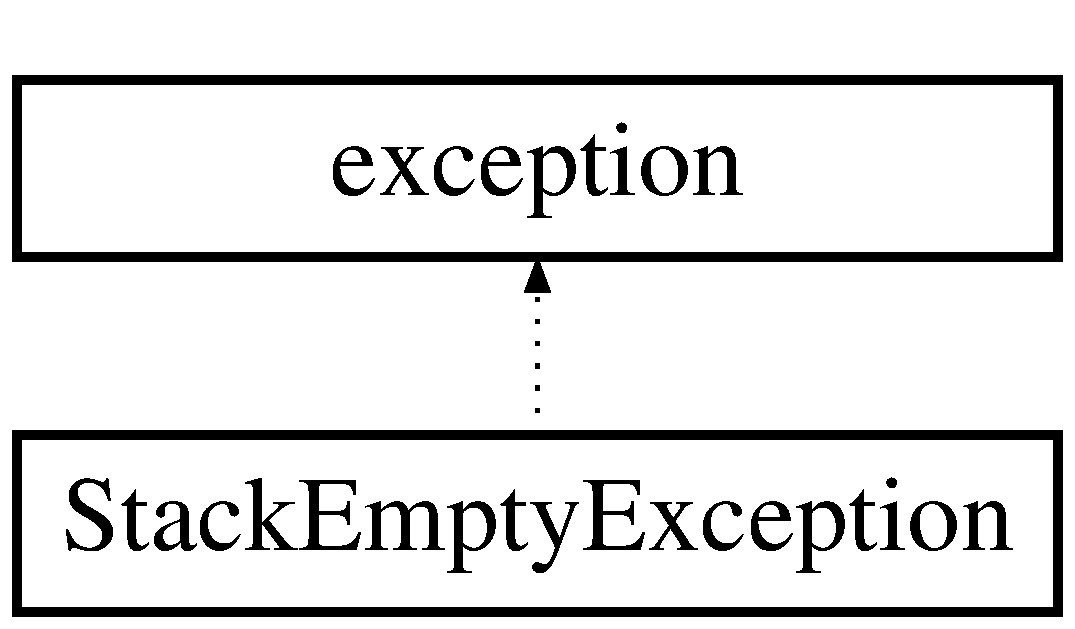
\includegraphics[height=2.000000cm]{class_stack_empty_exception}
\end{center}
\end{figure}
\subsection*{Public Member Functions}
\begin{DoxyCompactItemize}
\item 
\hyperlink{class_stack_empty_exception_a34c5802c05a3fe15ce7f3fd479fff6d9}{Stack\-Empty\-Exception} ()
\end{DoxyCompactItemize}


\subsection{Constructor \& Destructor Documentation}
\hypertarget{class_stack_empty_exception_a34c5802c05a3fe15ce7f3fd479fff6d9}{\index{Stack\-Empty\-Exception@{Stack\-Empty\-Exception}!Stack\-Empty\-Exception@{Stack\-Empty\-Exception}}
\index{Stack\-Empty\-Exception@{Stack\-Empty\-Exception}!StackEmptyException@{Stack\-Empty\-Exception}}
\subsubsection[{Stack\-Empty\-Exception}]{\setlength{\rightskip}{0pt plus 5cm}Stack\-Empty\-Exception\-::\-Stack\-Empty\-Exception (
\begin{DoxyParamCaption}
{}
\end{DoxyParamCaption}
)\hspace{0.3cm}{\ttfamily [inline]}}}\label{class_stack_empty_exception_a34c5802c05a3fe15ce7f3fd479fff6d9}


The documentation for this class was generated from the following file\-:\begin{DoxyCompactItemize}
\item 
H\-:/code/c++/zebra-\/zmachine-\/interpreter/zstack/zstack/\hyperlink{zstack_8h}{zstack.\-h}\end{DoxyCompactItemize}

\hypertarget{class_stack_full_exception}{\section{Stack\-Full\-Exception Class Reference}
\label{class_stack_full_exception}\index{Stack\-Full\-Exception@{Stack\-Full\-Exception}}
}


{\ttfamily \#include $<$zstack.\-h$>$}

Inheritance diagram for Stack\-Full\-Exception\-:\begin{figure}[H]
\begin{center}
\leavevmode
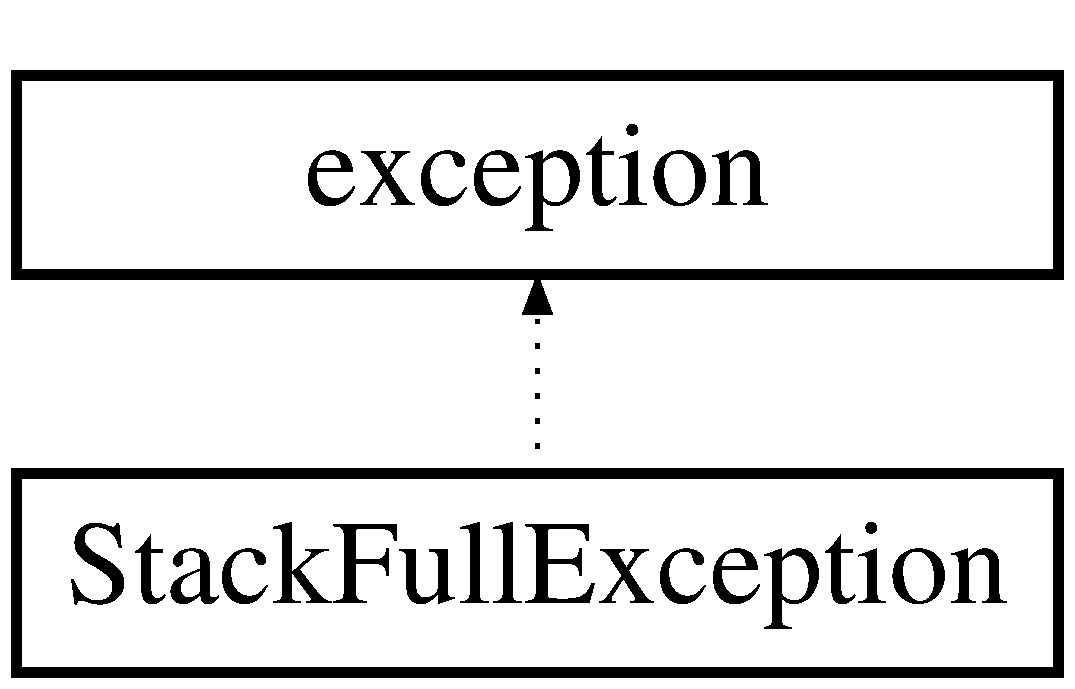
\includegraphics[height=2.000000cm]{class_stack_full_exception}
\end{center}
\end{figure}
\subsection*{Public Member Functions}
\begin{DoxyCompactItemize}
\item 
\hyperlink{class_stack_full_exception_a3d48d78b88670fa5b6f0a7b1a8f5bb35}{Stack\-Full\-Exception} ()
\end{DoxyCompactItemize}


\subsection{Constructor \& Destructor Documentation}
\hypertarget{class_stack_full_exception_a3d48d78b88670fa5b6f0a7b1a8f5bb35}{\index{Stack\-Full\-Exception@{Stack\-Full\-Exception}!Stack\-Full\-Exception@{Stack\-Full\-Exception}}
\index{Stack\-Full\-Exception@{Stack\-Full\-Exception}!StackFullException@{Stack\-Full\-Exception}}
\subsubsection[{Stack\-Full\-Exception}]{\setlength{\rightskip}{0pt plus 5cm}Stack\-Full\-Exception\-::\-Stack\-Full\-Exception (
\begin{DoxyParamCaption}
{}
\end{DoxyParamCaption}
)\hspace{0.3cm}{\ttfamily [inline]}}}\label{class_stack_full_exception_a3d48d78b88670fa5b6f0a7b1a8f5bb35}


The documentation for this class was generated from the following file\-:\begin{DoxyCompactItemize}
\item 
H\-:/code/c++/zebra-\/zmachine-\/interpreter/zstack/zstack/\hyperlink{zstack_8h}{zstack.\-h}\end{DoxyCompactItemize}

\hypertarget{structz_char_stringto_z_s_c_i_i_helper__save_state}{\section{z\-Char\-Stringto\-Z\-S\-C\-I\-I\-Helper\-\_\-save\-State Struct Reference}
\label{structz_char_stringto_z_s_c_i_i_helper__save_state}\index{z\-Char\-Stringto\-Z\-S\-C\-I\-I\-Helper\-\_\-save\-State@{z\-Char\-Stringto\-Z\-S\-C\-I\-I\-Helper\-\_\-save\-State}}
}
\subsection*{Public Member Functions}
\begin{DoxyCompactItemize}
\item 
\hyperlink{structz_char_stringto_z_s_c_i_i_helper__save_state_a1d1d18fcf6483873a0d933be3316273b}{z\-Char\-Stringto\-Z\-S\-C\-I\-I\-Helper\-\_\-save\-State} (int \hyperlink{structz_char_stringto_z_s_c_i_i_helper__save_state_ab9261aec1a4da3630a85089ba3d7ad21}{alpha\-Shift}, bool \hyperlink{structz_char_stringto_z_s_c_i_i_helper__save_state_a9e1b07c9af1aa49e625608ff3e86cc35}{shift\-Flag})
\end{DoxyCompactItemize}
\subsection*{Public Attributes}
\begin{DoxyCompactItemize}
\item 
int \hyperlink{structz_char_stringto_z_s_c_i_i_helper__save_state_ab9261aec1a4da3630a85089ba3d7ad21}{alpha\-Shift}
\item 
bool \hyperlink{structz_char_stringto_z_s_c_i_i_helper__save_state_a9e1b07c9af1aa49e625608ff3e86cc35}{shift\-Flag}
\end{DoxyCompactItemize}


\subsection{Constructor \& Destructor Documentation}
\hypertarget{structz_char_stringto_z_s_c_i_i_helper__save_state_a1d1d18fcf6483873a0d933be3316273b}{\index{z\-Char\-Stringto\-Z\-S\-C\-I\-I\-Helper\-\_\-save\-State@{z\-Char\-Stringto\-Z\-S\-C\-I\-I\-Helper\-\_\-save\-State}!z\-Char\-Stringto\-Z\-S\-C\-I\-I\-Helper\-\_\-save\-State@{z\-Char\-Stringto\-Z\-S\-C\-I\-I\-Helper\-\_\-save\-State}}
\index{z\-Char\-Stringto\-Z\-S\-C\-I\-I\-Helper\-\_\-save\-State@{z\-Char\-Stringto\-Z\-S\-C\-I\-I\-Helper\-\_\-save\-State}!zCharStringtoZSCIIHelper_saveState@{z\-Char\-Stringto\-Z\-S\-C\-I\-I\-Helper\-\_\-save\-State}}
\subsubsection[{z\-Char\-Stringto\-Z\-S\-C\-I\-I\-Helper\-\_\-save\-State}]{\setlength{\rightskip}{0pt plus 5cm}z\-Char\-Stringto\-Z\-S\-C\-I\-I\-Helper\-\_\-save\-State\-::z\-Char\-Stringto\-Z\-S\-C\-I\-I\-Helper\-\_\-save\-State (
\begin{DoxyParamCaption}
\item[{int}]{alpha\-Shift, }
\item[{bool}]{shift\-Flag}
\end{DoxyParamCaption}
)\hspace{0.3cm}{\ttfamily [inline]}}}\label{structz_char_stringto_z_s_c_i_i_helper__save_state_a1d1d18fcf6483873a0d933be3316273b}


\subsection{Member Data Documentation}
\hypertarget{structz_char_stringto_z_s_c_i_i_helper__save_state_ab9261aec1a4da3630a85089ba3d7ad21}{\index{z\-Char\-Stringto\-Z\-S\-C\-I\-I\-Helper\-\_\-save\-State@{z\-Char\-Stringto\-Z\-S\-C\-I\-I\-Helper\-\_\-save\-State}!alpha\-Shift@{alpha\-Shift}}
\index{alpha\-Shift@{alpha\-Shift}!zCharStringtoZSCIIHelper_saveState@{z\-Char\-Stringto\-Z\-S\-C\-I\-I\-Helper\-\_\-save\-State}}
\subsubsection[{alpha\-Shift}]{\setlength{\rightskip}{0pt plus 5cm}int z\-Char\-Stringto\-Z\-S\-C\-I\-I\-Helper\-\_\-save\-State\-::alpha\-Shift}}\label{structz_char_stringto_z_s_c_i_i_helper__save_state_ab9261aec1a4da3630a85089ba3d7ad21}
\hypertarget{structz_char_stringto_z_s_c_i_i_helper__save_state_a9e1b07c9af1aa49e625608ff3e86cc35}{\index{z\-Char\-Stringto\-Z\-S\-C\-I\-I\-Helper\-\_\-save\-State@{z\-Char\-Stringto\-Z\-S\-C\-I\-I\-Helper\-\_\-save\-State}!shift\-Flag@{shift\-Flag}}
\index{shift\-Flag@{shift\-Flag}!zCharStringtoZSCIIHelper_saveState@{z\-Char\-Stringto\-Z\-S\-C\-I\-I\-Helper\-\_\-save\-State}}
\subsubsection[{shift\-Flag}]{\setlength{\rightskip}{0pt plus 5cm}bool z\-Char\-Stringto\-Z\-S\-C\-I\-I\-Helper\-\_\-save\-State\-::shift\-Flag}}\label{structz_char_stringto_z_s_c_i_i_helper__save_state_a9e1b07c9af1aa49e625608ff3e86cc35}


The documentation for this struct was generated from the following file\-:\begin{DoxyCompactItemize}
\item 
H\-:/code/c++/zebra-\/zmachine-\/interpreter/ztext/ztext/\hyperlink{ztext_8cpp}{ztext.\-cpp}\end{DoxyCompactItemize}

\hypertarget{class_z_dictionary}{\section{Z\-Dictionary Class Reference}
\label{class_z_dictionary}\index{Z\-Dictionary@{Z\-Dictionary}}
}


{\ttfamily \#include $<$zdictionary.\-h$>$}

\subsection*{Public Member Functions}
\begin{DoxyCompactItemize}
\item 
\hyperlink{class_z_dictionary_a83a17daa48fba56e2ab0bf854f5a9318}{Z\-Dictionary} ()
\item 
\hyperlink{class_z_dictionary_aeca7959ca07a10b82e0179d4d17b9a22}{Z\-Dictionary} (\hyperlink{class_z_memory}{Z\-Memory} $\ast$z\-Mem\-Obj)  throw (\-Z\-Memory\-Read\-Out\-Of\-Bounds)
\item 
\hyperlink{class_z_dictionary_a302e3b83418ad1367f7bae991a270011}{$\sim$\-Z\-Dictionary} ()
\item 
\hyperlink{zglobal_8h_a6507dc55d18847442d5fb20b6c73fe73}{zword} \hyperlink{class_z_dictionary_a89cf4a5cbc0b770d8ac1aed19432d251}{get\-Dictionary\-Entry\-Addr} (\hyperlink{zglobal_8h_a718b4eb2652c286f4d42dc18a8e71a1a}{ulong} index)  throw (\-Illegal\-Dictionary\-Index)
\item 
\hyperlink{structz_dictionary_word}{z\-Dictionary\-Word} $\ast$$\ast$ \hyperlink{class_z_dictionary_a7ebd06ccc61abad818515d11cb0c39d3}{tokenize\-Z\-S\-C\-I\-I\-String} (\hyperlink{zglobal_8h_aef68b14f6fcd84f18d5b177486e4999b}{zchar} $\ast$\hyperlink{ztext_2ztext_2main_8cpp_ae991afe9cf5a78d591f33cce735aa9c7}{zstring})
\item 
\hyperlink{zglobal_8h_aef68b14f6fcd84f18d5b177486e4999b}{zchar} $\ast$ \hyperlink{class_z_dictionary_a1abd5cfd2321793d00ef62876bc3f3a9}{get\-Word\-Separators} ()
\end{DoxyCompactItemize}


\subsection{Constructor \& Destructor Documentation}
\hypertarget{class_z_dictionary_a83a17daa48fba56e2ab0bf854f5a9318}{\index{Z\-Dictionary@{Z\-Dictionary}!Z\-Dictionary@{Z\-Dictionary}}
\index{Z\-Dictionary@{Z\-Dictionary}!ZDictionary@{Z\-Dictionary}}
\subsubsection[{Z\-Dictionary}]{\setlength{\rightskip}{0pt plus 5cm}Z\-Dictionary\-::\-Z\-Dictionary (
\begin{DoxyParamCaption}
{}
\end{DoxyParamCaption}
)}}\label{class_z_dictionary_a83a17daa48fba56e2ab0bf854f5a9318}
\hypertarget{class_z_dictionary_aeca7959ca07a10b82e0179d4d17b9a22}{\index{Z\-Dictionary@{Z\-Dictionary}!Z\-Dictionary@{Z\-Dictionary}}
\index{Z\-Dictionary@{Z\-Dictionary}!ZDictionary@{Z\-Dictionary}}
\subsubsection[{Z\-Dictionary}]{\setlength{\rightskip}{0pt plus 5cm}Z\-Dictionary\-::\-Z\-Dictionary (
\begin{DoxyParamCaption}
\item[{{\bf Z\-Memory} $\ast$}]{z\-Mem\-Obj}
\end{DoxyParamCaption}
) throw  {\bf Z\-Memory\-Read\-Out\-Of\-Bounds}) }}\label{class_z_dictionary_aeca7959ca07a10b82e0179d4d17b9a22}
\hypertarget{class_z_dictionary_a302e3b83418ad1367f7bae991a270011}{\index{Z\-Dictionary@{Z\-Dictionary}!$\sim$\-Z\-Dictionary@{$\sim$\-Z\-Dictionary}}
\index{$\sim$\-Z\-Dictionary@{$\sim$\-Z\-Dictionary}!ZDictionary@{Z\-Dictionary}}
\subsubsection[{$\sim$\-Z\-Dictionary}]{\setlength{\rightskip}{0pt plus 5cm}Z\-Dictionary\-::$\sim$\-Z\-Dictionary (
\begin{DoxyParamCaption}
{}
\end{DoxyParamCaption}
)}}\label{class_z_dictionary_a302e3b83418ad1367f7bae991a270011}


\subsection{Member Function Documentation}
\hypertarget{class_z_dictionary_a89cf4a5cbc0b770d8ac1aed19432d251}{\index{Z\-Dictionary@{Z\-Dictionary}!get\-Dictionary\-Entry\-Addr@{get\-Dictionary\-Entry\-Addr}}
\index{get\-Dictionary\-Entry\-Addr@{get\-Dictionary\-Entry\-Addr}!ZDictionary@{Z\-Dictionary}}
\subsubsection[{get\-Dictionary\-Entry\-Addr}]{\setlength{\rightskip}{0pt plus 5cm}{\bf zword} Z\-Dictionary\-::get\-Dictionary\-Entry\-Addr (
\begin{DoxyParamCaption}
\item[{{\bf ulong}}]{index}
\end{DoxyParamCaption}
) throw  {\bf Illegal\-Dictionary\-Index}) }}\label{class_z_dictionary_a89cf4a5cbc0b770d8ac1aed19432d251}
\hypertarget{class_z_dictionary_a1abd5cfd2321793d00ef62876bc3f3a9}{\index{Z\-Dictionary@{Z\-Dictionary}!get\-Word\-Separators@{get\-Word\-Separators}}
\index{get\-Word\-Separators@{get\-Word\-Separators}!ZDictionary@{Z\-Dictionary}}
\subsubsection[{get\-Word\-Separators}]{\setlength{\rightskip}{0pt plus 5cm}{\bf zchar}$\ast$ Z\-Dictionary\-::get\-Word\-Separators (
\begin{DoxyParamCaption}
{}
\end{DoxyParamCaption}
)\hspace{0.3cm}{\ttfamily [inline]}}}\label{class_z_dictionary_a1abd5cfd2321793d00ef62876bc3f3a9}
\hypertarget{class_z_dictionary_a7ebd06ccc61abad818515d11cb0c39d3}{\index{Z\-Dictionary@{Z\-Dictionary}!tokenize\-Z\-S\-C\-I\-I\-String@{tokenize\-Z\-S\-C\-I\-I\-String}}
\index{tokenize\-Z\-S\-C\-I\-I\-String@{tokenize\-Z\-S\-C\-I\-I\-String}!ZDictionary@{Z\-Dictionary}}
\subsubsection[{tokenize\-Z\-S\-C\-I\-I\-String}]{\setlength{\rightskip}{0pt plus 5cm}Z\-S\-C\-I\-I\-Dictionary\-Token $\ast$$\ast$ Z\-Dictionary\-::tokenize\-Z\-S\-C\-I\-I\-String (
\begin{DoxyParamCaption}
\item[{{\bf zchar} $\ast$}]{zstring}
\end{DoxyParamCaption}
)}}\label{class_z_dictionary_a7ebd06ccc61abad818515d11cb0c39d3}


The documentation for this class was generated from the following files\-:\begin{DoxyCompactItemize}
\item 
H\-:/code/c++/zebra-\/zmachine-\/interpreter/zdictionary/zdictionary/\hyperlink{zdictionary_8h}{zdictionary.\-h}\item 
H\-:/code/c++/zebra-\/zmachine-\/interpreter/zdictionary/zdictionary/\hyperlink{zdictionary_8cpp}{zdictionary.\-cpp}\end{DoxyCompactItemize}

\hypertarget{structz_dictionary_word}{\section{z\-Dictionary\-Word Struct Reference}
\label{structz_dictionary_word}\index{z\-Dictionary\-Word@{z\-Dictionary\-Word}}
}


{\ttfamily \#include $<$zdictionary.\-h$>$}

\subsection*{Public Member Functions}
\begin{DoxyCompactItemize}
\item 
\hyperlink{structz_dictionary_word_ac7a4bfd1848c4bb17eefa6933ec23495}{z\-Dictionary\-Word} ()
\item 
\hyperlink{structz_dictionary_word_a5680db4b9d0fd362ba9b50069d64540a}{z\-Dictionary\-Word} (\hyperlink{zglobal_8h_aef68b14f6fcd84f18d5b177486e4999b}{zchar} $\ast$\hyperlink{structz_dictionary_word_a052383f6650a13c20731dc2e790614ab}{word\-Data})
\item 
const \hyperlink{structz_dictionary_word}{z\-Dictionary\-Word} \& \hyperlink{structz_dictionary_word_a8c2f286835d48c3ab46f9530d91c2219}{operator=} (const \hyperlink{structz_dictionary_word}{z\-Dictionary\-Word} \&a)
\end{DoxyCompactItemize}
\subsection*{Public Attributes}
\begin{DoxyCompactItemize}
\item 
\hyperlink{zglobal_8h_aef68b14f6fcd84f18d5b177486e4999b}{zchar} $\ast$ \hyperlink{structz_dictionary_word_a052383f6650a13c20731dc2e790614ab}{word\-Data}
\end{DoxyCompactItemize}


\subsection{Constructor \& Destructor Documentation}
\hypertarget{structz_dictionary_word_ac7a4bfd1848c4bb17eefa6933ec23495}{\index{z\-Dictionary\-Word@{z\-Dictionary\-Word}!z\-Dictionary\-Word@{z\-Dictionary\-Word}}
\index{z\-Dictionary\-Word@{z\-Dictionary\-Word}!zDictionaryWord@{z\-Dictionary\-Word}}
\subsubsection[{z\-Dictionary\-Word}]{\setlength{\rightskip}{0pt plus 5cm}z\-Dictionary\-Word\-::z\-Dictionary\-Word (
\begin{DoxyParamCaption}
{}
\end{DoxyParamCaption}
)\hspace{0.3cm}{\ttfamily [inline]}}}\label{structz_dictionary_word_ac7a4bfd1848c4bb17eefa6933ec23495}
\hypertarget{structz_dictionary_word_a5680db4b9d0fd362ba9b50069d64540a}{\index{z\-Dictionary\-Word@{z\-Dictionary\-Word}!z\-Dictionary\-Word@{z\-Dictionary\-Word}}
\index{z\-Dictionary\-Word@{z\-Dictionary\-Word}!zDictionaryWord@{z\-Dictionary\-Word}}
\subsubsection[{z\-Dictionary\-Word}]{\setlength{\rightskip}{0pt plus 5cm}z\-Dictionary\-Word\-::z\-Dictionary\-Word (
\begin{DoxyParamCaption}
\item[{{\bf zchar} $\ast$}]{word\-Data}
\end{DoxyParamCaption}
)\hspace{0.3cm}{\ttfamily [inline]}}}\label{structz_dictionary_word_a5680db4b9d0fd362ba9b50069d64540a}


\subsection{Member Function Documentation}
\hypertarget{structz_dictionary_word_a8c2f286835d48c3ab46f9530d91c2219}{\index{z\-Dictionary\-Word@{z\-Dictionary\-Word}!operator=@{operator=}}
\index{operator=@{operator=}!zDictionaryWord@{z\-Dictionary\-Word}}
\subsubsection[{operator=}]{\setlength{\rightskip}{0pt plus 5cm}const {\bf z\-Dictionary\-Word}\& z\-Dictionary\-Word\-::operator= (
\begin{DoxyParamCaption}
\item[{const {\bf z\-Dictionary\-Word} \&}]{a}
\end{DoxyParamCaption}
)\hspace{0.3cm}{\ttfamily [inline]}}}\label{structz_dictionary_word_a8c2f286835d48c3ab46f9530d91c2219}


\subsection{Member Data Documentation}
\hypertarget{structz_dictionary_word_a052383f6650a13c20731dc2e790614ab}{\index{z\-Dictionary\-Word@{z\-Dictionary\-Word}!word\-Data@{word\-Data}}
\index{word\-Data@{word\-Data}!zDictionaryWord@{z\-Dictionary\-Word}}
\subsubsection[{word\-Data}]{\setlength{\rightskip}{0pt plus 5cm}{\bf zchar}$\ast$ z\-Dictionary\-Word\-::word\-Data}}\label{structz_dictionary_word_a052383f6650a13c20731dc2e790614ab}


The documentation for this struct was generated from the following file\-:\begin{DoxyCompactItemize}
\item 
H\-:/code/c++/zebra-\/zmachine-\/interpreter/zdictionary/zdictionary/\hyperlink{zdictionary_8h}{zdictionary.\-h}\end{DoxyCompactItemize}

\hypertarget{class_z_error}{\section{Z\-Error Class Reference}
\label{class_z_error}\index{Z\-Error@{Z\-Error}}
}


{\ttfamily \#include $<$zerror.\-h$>$}

\subsection*{Public Types}
\begin{DoxyCompactItemize}
\item 
enum \hyperlink{class_z_error_a0b55bf98ee62a9614e249b5ef6d184f9}{flush} \{ \hyperlink{class_z_error_a0b55bf98ee62a9614e249b5ef6d184f9acc61b827431a7b09a95990c952ca1830}{F\-L\-U\-S\-H\-\_\-\-I\-M\-M\-E\-D\-I\-A\-T\-E}, 
\hyperlink{class_z_error_a0b55bf98ee62a9614e249b5ef6d184f9a0460ce1a3b526457ce5f08fac4572831}{F\-L\-U\-S\-H\-\_\-\-O\-N\-D\-E\-M\-A\-N\-D}
 \}
\end{DoxyCompactItemize}
\subsection*{Public Member Functions}
\begin{DoxyCompactItemize}
\item 
\hyperlink{class_z_error_a787f55d0c8b3c3777894249983aa83d4}{Z\-Error} ()
\item 
\hyperlink{class_z_error_a74830cdc570fb79a697566e16fadfd58}{$\sim$\-Z\-Error} ()
\item 
void \hyperlink{class_z_error_a46b084ba65b66073549c19f826d2f363}{add\-Error} (string error\-Msg)
\item 
void \hyperlink{class_z_error_a4c01e2544b6c981c63d0b354f5c21be1}{set\-Buffer\-Flush} (int val)
\item 
void \hyperlink{class_z_error_a607bcf825c9825e66e8ba91c75f79b04}{flush\-Buffer} ()
\end{DoxyCompactItemize}


\subsection{Member Enumeration Documentation}
\hypertarget{class_z_error_a0b55bf98ee62a9614e249b5ef6d184f9}{\index{Z\-Error@{Z\-Error}!flush@{flush}}
\index{flush@{flush}!ZError@{Z\-Error}}
\subsubsection[{flush}]{\setlength{\rightskip}{0pt plus 5cm}enum {\bf Z\-Error\-::flush}}}\label{class_z_error_a0b55bf98ee62a9614e249b5ef6d184f9}
\begin{Desc}
\item[Enumerator]\par
\begin{description}
\index{F\-L\-U\-S\-H\-\_\-\-I\-M\-M\-E\-D\-I\-A\-T\-E@{F\-L\-U\-S\-H\-\_\-\-I\-M\-M\-E\-D\-I\-A\-T\-E}!Z\-Error@{Z\-Error}}\index{Z\-Error@{Z\-Error}!F\-L\-U\-S\-H\-\_\-\-I\-M\-M\-E\-D\-I\-A\-T\-E@{F\-L\-U\-S\-H\-\_\-\-I\-M\-M\-E\-D\-I\-A\-T\-E}}\item[{\em 
\hypertarget{class_z_error_a0b55bf98ee62a9614e249b5ef6d184f9acc61b827431a7b09a95990c952ca1830}{F\-L\-U\-S\-H\-\_\-\-I\-M\-M\-E\-D\-I\-A\-T\-E}\label{class_z_error_a0b55bf98ee62a9614e249b5ef6d184f9acc61b827431a7b09a95990c952ca1830}
}]\index{F\-L\-U\-S\-H\-\_\-\-O\-N\-D\-E\-M\-A\-N\-D@{F\-L\-U\-S\-H\-\_\-\-O\-N\-D\-E\-M\-A\-N\-D}!Z\-Error@{Z\-Error}}\index{Z\-Error@{Z\-Error}!F\-L\-U\-S\-H\-\_\-\-O\-N\-D\-E\-M\-A\-N\-D@{F\-L\-U\-S\-H\-\_\-\-O\-N\-D\-E\-M\-A\-N\-D}}\item[{\em 
\hypertarget{class_z_error_a0b55bf98ee62a9614e249b5ef6d184f9a0460ce1a3b526457ce5f08fac4572831}{F\-L\-U\-S\-H\-\_\-\-O\-N\-D\-E\-M\-A\-N\-D}\label{class_z_error_a0b55bf98ee62a9614e249b5ef6d184f9a0460ce1a3b526457ce5f08fac4572831}
}]\end{description}
\end{Desc}


\subsection{Constructor \& Destructor Documentation}
\hypertarget{class_z_error_a787f55d0c8b3c3777894249983aa83d4}{\index{Z\-Error@{Z\-Error}!Z\-Error@{Z\-Error}}
\index{Z\-Error@{Z\-Error}!ZError@{Z\-Error}}
\subsubsection[{Z\-Error}]{\setlength{\rightskip}{0pt plus 5cm}Z\-Error\-::\-Z\-Error (
\begin{DoxyParamCaption}
{}
\end{DoxyParamCaption}
)\hspace{0.3cm}{\ttfamily [inline]}}}\label{class_z_error_a787f55d0c8b3c3777894249983aa83d4}
\hypertarget{class_z_error_a74830cdc570fb79a697566e16fadfd58}{\index{Z\-Error@{Z\-Error}!$\sim$\-Z\-Error@{$\sim$\-Z\-Error}}
\index{$\sim$\-Z\-Error@{$\sim$\-Z\-Error}!ZError@{Z\-Error}}
\subsubsection[{$\sim$\-Z\-Error}]{\setlength{\rightskip}{0pt plus 5cm}Z\-Error\-::$\sim$\-Z\-Error (
\begin{DoxyParamCaption}
{}
\end{DoxyParamCaption}
)\hspace{0.3cm}{\ttfamily [inline]}}}\label{class_z_error_a74830cdc570fb79a697566e16fadfd58}


\subsection{Member Function Documentation}
\hypertarget{class_z_error_a46b084ba65b66073549c19f826d2f363}{\index{Z\-Error@{Z\-Error}!add\-Error@{add\-Error}}
\index{add\-Error@{add\-Error}!ZError@{Z\-Error}}
\subsubsection[{add\-Error}]{\setlength{\rightskip}{0pt plus 5cm}void Z\-Error\-::add\-Error (
\begin{DoxyParamCaption}
\item[{string}]{error\-Msg}
\end{DoxyParamCaption}
)}}\label{class_z_error_a46b084ba65b66073549c19f826d2f363}
\hypertarget{class_z_error_a607bcf825c9825e66e8ba91c75f79b04}{\index{Z\-Error@{Z\-Error}!flush\-Buffer@{flush\-Buffer}}
\index{flush\-Buffer@{flush\-Buffer}!ZError@{Z\-Error}}
\subsubsection[{flush\-Buffer}]{\setlength{\rightskip}{0pt plus 5cm}void Z\-Error\-::flush\-Buffer (
\begin{DoxyParamCaption}
{}
\end{DoxyParamCaption}
)}}\label{class_z_error_a607bcf825c9825e66e8ba91c75f79b04}
\hypertarget{class_z_error_a4c01e2544b6c981c63d0b354f5c21be1}{\index{Z\-Error@{Z\-Error}!set\-Buffer\-Flush@{set\-Buffer\-Flush}}
\index{set\-Buffer\-Flush@{set\-Buffer\-Flush}!ZError@{Z\-Error}}
\subsubsection[{set\-Buffer\-Flush}]{\setlength{\rightskip}{0pt plus 5cm}void Z\-Error\-::set\-Buffer\-Flush (
\begin{DoxyParamCaption}
\item[{int}]{val}
\end{DoxyParamCaption}
)}}\label{class_z_error_a4c01e2544b6c981c63d0b354f5c21be1}


The documentation for this class was generated from the following files\-:\begin{DoxyCompactItemize}
\item 
H\-:/code/c++/zebra-\/zmachine-\/interpreter/zerror/zerror/\hyperlink{zerror_8h}{zerror.\-h}\item 
H\-:/code/c++/zebra-\/zmachine-\/interpreter/zerror/zerror/\hyperlink{zerror_8cpp}{zerror.\-cpp}\end{DoxyCompactItemize}

\hypertarget{class_z_memory}{\section{Z\-Memory Class Reference}
\label{class_z_memory}\index{Z\-Memory@{Z\-Memory}}
}


{\ttfamily \#include $<$zmemory.\-h$>$}

\subsection*{Public Member Functions}
\begin{DoxyCompactItemize}
\item 
\hyperlink{zglobal_8h_aab4ef09707609e67bcc5a552cde255d2}{zbyte} $\ast$ \hyperlink{class_z_memory_a701e72664f8f28c5b7359e767458b147}{get\-Raw\-Data\-Ptr} ()
\item 
\hyperlink{zglobal_8h_a718b4eb2652c286f4d42dc18a8e71a1a}{ulong} \hyperlink{class_z_memory_a855d50c042e28fde0b54ad003be317c9}{get\-Mem\-Size} ()
\item 
\hyperlink{zglobal_8h_a718b4eb2652c286f4d42dc18a8e71a1a}{ulong} \hyperlink{class_z_memory_af91d5e9664afa35b54694c6dfe8f6700}{get\-Z\-Dynamic\-Memory\-Lower} ()
\item 
\hyperlink{zglobal_8h_a718b4eb2652c286f4d42dc18a8e71a1a}{ulong} \hyperlink{class_z_memory_ae2790a344ca08584a6fb2f3a3d19bbc3}{get\-Z\-Dynamic\-Memory\-Upper} ()
\item 
\hyperlink{zglobal_8h_a718b4eb2652c286f4d42dc18a8e71a1a}{ulong} \hyperlink{class_z_memory_a177dc4a6dc2390a18a51e91ffccdf5d3}{get\-Z\-Static\-Memory\-Lower} ()
\item 
\hyperlink{zglobal_8h_a718b4eb2652c286f4d42dc18a8e71a1a}{ulong} \hyperlink{class_z_memory_a9c0e44da941991913cc18adc50029d91}{get\-Z\-Static\-Memory\-Upper} ()
\item 
\hyperlink{zglobal_8h_a718b4eb2652c286f4d42dc18a8e71a1a}{ulong} \hyperlink{class_z_memory_a43f47592c50fb8521e21805796a25be9}{get\-Z\-High\-Memory\-Lower} ()
\item 
\hyperlink{zglobal_8h_a718b4eb2652c286f4d42dc18a8e71a1a}{ulong} \hyperlink{class_z_memory_a579f76a2b85fad4e7e96a0bf77ef7f94}{get\-Z\-High\-Memory\-Upper} ()
\item 
\hyperlink{zglobal_8h_a6507dc55d18847442d5fb20b6c73fe73}{zword} \hyperlink{class_z_memory_a894c694789b32d085e7e33e486419e94}{read\-Z\-Word} (\hyperlink{zglobal_8h_a6507dc55d18847442d5fb20b6c73fe73}{zword} addr)  throw (\-Z\-Memory\-Read\-Out\-Of\-Bounds)
\item 
\hyperlink{zglobal_8h_a6507dc55d18847442d5fb20b6c73fe73}{zword} \hyperlink{class_z_memory_ad74221329cb16f4b08cb9b6abc2e1c10}{read\-Z\-Word\-Packed\-Addr} (\hyperlink{zglobal_8h_a6507dc55d18847442d5fb20b6c73fe73}{zword} addr)  throw (\-Z\-Memory\-Read\-Out\-Of\-Bounds)
\item 
\hyperlink{zglobal_8h_aab4ef09707609e67bcc5a552cde255d2}{zbyte} \hyperlink{class_z_memory_a6ca3e706d4fef287677eb1171e9d88d7}{read\-Z\-Byte} (\hyperlink{zglobal_8h_a6507dc55d18847442d5fb20b6c73fe73}{zword} addr)  throw (\-Z\-Memory\-Read\-Out\-Of\-Bounds)
\item 
\hyperlink{zglobal_8h_aab4ef09707609e67bcc5a552cde255d2}{zbyte} \hyperlink{class_z_memory_aff0202af0bac630b9119196bc70fd087}{read\-Z\-Byte\-Packed\-Addr} (\hyperlink{zglobal_8h_a6507dc55d18847442d5fb20b6c73fe73}{zword} addr)  throw (\-Z\-Memory\-Read\-Out\-Of\-Bounds)
\item 
void \hyperlink{class_z_memory_a2e261ca55a5ca5f047a345f9478579fd}{store\-Z\-Word} (\hyperlink{zglobal_8h_a6507dc55d18847442d5fb20b6c73fe73}{zword} addr, \hyperlink{zglobal_8h_a6507dc55d18847442d5fb20b6c73fe73}{zword} data)  throw (\-Z\-Memory\-Write\-Out\-Of\-Bounds)
\item 
void \hyperlink{class_z_memory_abf715d1780c0ec3f8e399d4c4d24b083}{store\-Z\-Word\-Packed\-Addr} (\hyperlink{zglobal_8h_a6507dc55d18847442d5fb20b6c73fe73}{zword} addr, \hyperlink{zglobal_8h_a6507dc55d18847442d5fb20b6c73fe73}{zword} data)  throw (\-Z\-Memory\-Write\-Out\-Of\-Bounds)
\item 
void \hyperlink{class_z_memory_a8ee9c13cf3c1be05093e4725e3f54822}{store\-Z\-Byte} (\hyperlink{zglobal_8h_a6507dc55d18847442d5fb20b6c73fe73}{zword} addr, \hyperlink{zglobal_8h_aab4ef09707609e67bcc5a552cde255d2}{zbyte} data)  throw (\-Z\-Memory\-Write\-Out\-Of\-Bounds)
\item 
void \hyperlink{class_z_memory_a1620640052e61e1118305329f49eea2f}{store\-Z\-Byte\-Packed\-Addr} (\hyperlink{zglobal_8h_a6507dc55d18847442d5fb20b6c73fe73}{zword} addr, \hyperlink{zglobal_8h_aab4ef09707609e67bcc5a552cde255d2}{zbyte} data)  throw (\-Z\-Memory\-Write\-Out\-Of\-Bounds)
\item 
\hyperlink{class_z_memory_a83f209a355f1d154be6037b7e6cc4f21}{Z\-Memory} ()
\item 
\hyperlink{class_z_memory_a5c7d09e5e24dbe1fb9b013bba0320b62}{Z\-Memory} (\hyperlink{zglobal_8h_aab4ef09707609e67bcc5a552cde255d2}{zbyte} $\ast$z\-Data, \hyperlink{zglobal_8h_a718b4eb2652c286f4d42dc18a8e71a1a}{ulong} z\-Data\-Length)
\item 
\hyperlink{class_z_memory_aa98d6ee3984021ff330fdeb1158a23f1}{$\sim$\-Z\-Memory} ()
\end{DoxyCompactItemize}


\subsection{Constructor \& Destructor Documentation}
\hypertarget{class_z_memory_a83f209a355f1d154be6037b7e6cc4f21}{\index{Z\-Memory@{Z\-Memory}!Z\-Memory@{Z\-Memory}}
\index{Z\-Memory@{Z\-Memory}!ZMemory@{Z\-Memory}}
\subsubsection[{Z\-Memory}]{\setlength{\rightskip}{0pt plus 5cm}Z\-Memory\-::\-Z\-Memory (
\begin{DoxyParamCaption}
{}
\end{DoxyParamCaption}
)}}\label{class_z_memory_a83f209a355f1d154be6037b7e6cc4f21}
\hypertarget{class_z_memory_a5c7d09e5e24dbe1fb9b013bba0320b62}{\index{Z\-Memory@{Z\-Memory}!Z\-Memory@{Z\-Memory}}
\index{Z\-Memory@{Z\-Memory}!ZMemory@{Z\-Memory}}
\subsubsection[{Z\-Memory}]{\setlength{\rightskip}{0pt plus 5cm}Z\-Memory\-::\-Z\-Memory (
\begin{DoxyParamCaption}
\item[{{\bf zbyte} $\ast$}]{z\-Data, }
\item[{{\bf ulong}}]{z\-Data\-Length}
\end{DoxyParamCaption}
)}}\label{class_z_memory_a5c7d09e5e24dbe1fb9b013bba0320b62}
\hypertarget{class_z_memory_aa98d6ee3984021ff330fdeb1158a23f1}{\index{Z\-Memory@{Z\-Memory}!$\sim$\-Z\-Memory@{$\sim$\-Z\-Memory}}
\index{$\sim$\-Z\-Memory@{$\sim$\-Z\-Memory}!ZMemory@{Z\-Memory}}
\subsubsection[{$\sim$\-Z\-Memory}]{\setlength{\rightskip}{0pt plus 5cm}Z\-Memory\-::$\sim$\-Z\-Memory (
\begin{DoxyParamCaption}
{}
\end{DoxyParamCaption}
)}}\label{class_z_memory_aa98d6ee3984021ff330fdeb1158a23f1}


\subsection{Member Function Documentation}
\hypertarget{class_z_memory_a855d50c042e28fde0b54ad003be317c9}{\index{Z\-Memory@{Z\-Memory}!get\-Mem\-Size@{get\-Mem\-Size}}
\index{get\-Mem\-Size@{get\-Mem\-Size}!ZMemory@{Z\-Memory}}
\subsubsection[{get\-Mem\-Size}]{\setlength{\rightskip}{0pt plus 5cm}{\bf ulong} Z\-Memory\-::get\-Mem\-Size (
\begin{DoxyParamCaption}
{}
\end{DoxyParamCaption}
)\hspace{0.3cm}{\ttfamily [inline]}}}\label{class_z_memory_a855d50c042e28fde0b54ad003be317c9}
\hypertarget{class_z_memory_a701e72664f8f28c5b7359e767458b147}{\index{Z\-Memory@{Z\-Memory}!get\-Raw\-Data\-Ptr@{get\-Raw\-Data\-Ptr}}
\index{get\-Raw\-Data\-Ptr@{get\-Raw\-Data\-Ptr}!ZMemory@{Z\-Memory}}
\subsubsection[{get\-Raw\-Data\-Ptr}]{\setlength{\rightskip}{0pt plus 5cm}{\bf zbyte}$\ast$ Z\-Memory\-::get\-Raw\-Data\-Ptr (
\begin{DoxyParamCaption}
{}
\end{DoxyParamCaption}
)\hspace{0.3cm}{\ttfamily [inline]}}}\label{class_z_memory_a701e72664f8f28c5b7359e767458b147}
\hypertarget{class_z_memory_af91d5e9664afa35b54694c6dfe8f6700}{\index{Z\-Memory@{Z\-Memory}!get\-Z\-Dynamic\-Memory\-Lower@{get\-Z\-Dynamic\-Memory\-Lower}}
\index{get\-Z\-Dynamic\-Memory\-Lower@{get\-Z\-Dynamic\-Memory\-Lower}!ZMemory@{Z\-Memory}}
\subsubsection[{get\-Z\-Dynamic\-Memory\-Lower}]{\setlength{\rightskip}{0pt plus 5cm}{\bf ulong} Z\-Memory\-::get\-Z\-Dynamic\-Memory\-Lower (
\begin{DoxyParamCaption}
{}
\end{DoxyParamCaption}
)\hspace{0.3cm}{\ttfamily [inline]}}}\label{class_z_memory_af91d5e9664afa35b54694c6dfe8f6700}
\hypertarget{class_z_memory_ae2790a344ca08584a6fb2f3a3d19bbc3}{\index{Z\-Memory@{Z\-Memory}!get\-Z\-Dynamic\-Memory\-Upper@{get\-Z\-Dynamic\-Memory\-Upper}}
\index{get\-Z\-Dynamic\-Memory\-Upper@{get\-Z\-Dynamic\-Memory\-Upper}!ZMemory@{Z\-Memory}}
\subsubsection[{get\-Z\-Dynamic\-Memory\-Upper}]{\setlength{\rightskip}{0pt plus 5cm}{\bf ulong} Z\-Memory\-::get\-Z\-Dynamic\-Memory\-Upper (
\begin{DoxyParamCaption}
{}
\end{DoxyParamCaption}
)\hspace{0.3cm}{\ttfamily [inline]}}}\label{class_z_memory_ae2790a344ca08584a6fb2f3a3d19bbc3}
\hypertarget{class_z_memory_a43f47592c50fb8521e21805796a25be9}{\index{Z\-Memory@{Z\-Memory}!get\-Z\-High\-Memory\-Lower@{get\-Z\-High\-Memory\-Lower}}
\index{get\-Z\-High\-Memory\-Lower@{get\-Z\-High\-Memory\-Lower}!ZMemory@{Z\-Memory}}
\subsubsection[{get\-Z\-High\-Memory\-Lower}]{\setlength{\rightskip}{0pt plus 5cm}{\bf ulong} Z\-Memory\-::get\-Z\-High\-Memory\-Lower (
\begin{DoxyParamCaption}
{}
\end{DoxyParamCaption}
)\hspace{0.3cm}{\ttfamily [inline]}}}\label{class_z_memory_a43f47592c50fb8521e21805796a25be9}
\hypertarget{class_z_memory_a579f76a2b85fad4e7e96a0bf77ef7f94}{\index{Z\-Memory@{Z\-Memory}!get\-Z\-High\-Memory\-Upper@{get\-Z\-High\-Memory\-Upper}}
\index{get\-Z\-High\-Memory\-Upper@{get\-Z\-High\-Memory\-Upper}!ZMemory@{Z\-Memory}}
\subsubsection[{get\-Z\-High\-Memory\-Upper}]{\setlength{\rightskip}{0pt plus 5cm}{\bf ulong} Z\-Memory\-::get\-Z\-High\-Memory\-Upper (
\begin{DoxyParamCaption}
{}
\end{DoxyParamCaption}
)\hspace{0.3cm}{\ttfamily [inline]}}}\label{class_z_memory_a579f76a2b85fad4e7e96a0bf77ef7f94}
\hypertarget{class_z_memory_a177dc4a6dc2390a18a51e91ffccdf5d3}{\index{Z\-Memory@{Z\-Memory}!get\-Z\-Static\-Memory\-Lower@{get\-Z\-Static\-Memory\-Lower}}
\index{get\-Z\-Static\-Memory\-Lower@{get\-Z\-Static\-Memory\-Lower}!ZMemory@{Z\-Memory}}
\subsubsection[{get\-Z\-Static\-Memory\-Lower}]{\setlength{\rightskip}{0pt plus 5cm}{\bf ulong} Z\-Memory\-::get\-Z\-Static\-Memory\-Lower (
\begin{DoxyParamCaption}
{}
\end{DoxyParamCaption}
)\hspace{0.3cm}{\ttfamily [inline]}}}\label{class_z_memory_a177dc4a6dc2390a18a51e91ffccdf5d3}
\hypertarget{class_z_memory_a9c0e44da941991913cc18adc50029d91}{\index{Z\-Memory@{Z\-Memory}!get\-Z\-Static\-Memory\-Upper@{get\-Z\-Static\-Memory\-Upper}}
\index{get\-Z\-Static\-Memory\-Upper@{get\-Z\-Static\-Memory\-Upper}!ZMemory@{Z\-Memory}}
\subsubsection[{get\-Z\-Static\-Memory\-Upper}]{\setlength{\rightskip}{0pt plus 5cm}{\bf ulong} Z\-Memory\-::get\-Z\-Static\-Memory\-Upper (
\begin{DoxyParamCaption}
{}
\end{DoxyParamCaption}
)\hspace{0.3cm}{\ttfamily [inline]}}}\label{class_z_memory_a9c0e44da941991913cc18adc50029d91}
\hypertarget{class_z_memory_a6ca3e706d4fef287677eb1171e9d88d7}{\index{Z\-Memory@{Z\-Memory}!read\-Z\-Byte@{read\-Z\-Byte}}
\index{read\-Z\-Byte@{read\-Z\-Byte}!ZMemory@{Z\-Memory}}
\subsubsection[{read\-Z\-Byte}]{\setlength{\rightskip}{0pt plus 5cm}{\bf zbyte} Z\-Memory\-::read\-Z\-Byte (
\begin{DoxyParamCaption}
\item[{{\bf zword}}]{addr}
\end{DoxyParamCaption}
) throw  {\bf Z\-Memory\-Read\-Out\-Of\-Bounds}) }}\label{class_z_memory_a6ca3e706d4fef287677eb1171e9d88d7}
\hypertarget{class_z_memory_aff0202af0bac630b9119196bc70fd087}{\index{Z\-Memory@{Z\-Memory}!read\-Z\-Byte\-Packed\-Addr@{read\-Z\-Byte\-Packed\-Addr}}
\index{read\-Z\-Byte\-Packed\-Addr@{read\-Z\-Byte\-Packed\-Addr}!ZMemory@{Z\-Memory}}
\subsubsection[{read\-Z\-Byte\-Packed\-Addr}]{\setlength{\rightskip}{0pt plus 5cm}{\bf zbyte} Z\-Memory\-::read\-Z\-Byte\-Packed\-Addr (
\begin{DoxyParamCaption}
\item[{{\bf zword}}]{addr}
\end{DoxyParamCaption}
) throw  {\bf Z\-Memory\-Read\-Out\-Of\-Bounds}) }}\label{class_z_memory_aff0202af0bac630b9119196bc70fd087}
\hypertarget{class_z_memory_a894c694789b32d085e7e33e486419e94}{\index{Z\-Memory@{Z\-Memory}!read\-Z\-Word@{read\-Z\-Word}}
\index{read\-Z\-Word@{read\-Z\-Word}!ZMemory@{Z\-Memory}}
\subsubsection[{read\-Z\-Word}]{\setlength{\rightskip}{0pt plus 5cm}{\bf zword} Z\-Memory\-::read\-Z\-Word (
\begin{DoxyParamCaption}
\item[{{\bf zword}}]{addr}
\end{DoxyParamCaption}
) throw  {\bf Z\-Memory\-Read\-Out\-Of\-Bounds}) }}\label{class_z_memory_a894c694789b32d085e7e33e486419e94}
\hypertarget{class_z_memory_ad74221329cb16f4b08cb9b6abc2e1c10}{\index{Z\-Memory@{Z\-Memory}!read\-Z\-Word\-Packed\-Addr@{read\-Z\-Word\-Packed\-Addr}}
\index{read\-Z\-Word\-Packed\-Addr@{read\-Z\-Word\-Packed\-Addr}!ZMemory@{Z\-Memory}}
\subsubsection[{read\-Z\-Word\-Packed\-Addr}]{\setlength{\rightskip}{0pt plus 5cm}{\bf zword} Z\-Memory\-::read\-Z\-Word\-Packed\-Addr (
\begin{DoxyParamCaption}
\item[{{\bf zword}}]{addr}
\end{DoxyParamCaption}
) throw  {\bf Z\-Memory\-Read\-Out\-Of\-Bounds}) }}\label{class_z_memory_ad74221329cb16f4b08cb9b6abc2e1c10}
\hypertarget{class_z_memory_a8ee9c13cf3c1be05093e4725e3f54822}{\index{Z\-Memory@{Z\-Memory}!store\-Z\-Byte@{store\-Z\-Byte}}
\index{store\-Z\-Byte@{store\-Z\-Byte}!ZMemory@{Z\-Memory}}
\subsubsection[{store\-Z\-Byte}]{\setlength{\rightskip}{0pt plus 5cm}void Z\-Memory\-::store\-Z\-Byte (
\begin{DoxyParamCaption}
\item[{{\bf zword}}]{addr, }
\item[{{\bf zbyte}}]{data}
\end{DoxyParamCaption}
) throw  {\bf Z\-Memory\-Write\-Out\-Of\-Bounds}) }}\label{class_z_memory_a8ee9c13cf3c1be05093e4725e3f54822}
\hypertarget{class_z_memory_a1620640052e61e1118305329f49eea2f}{\index{Z\-Memory@{Z\-Memory}!store\-Z\-Byte\-Packed\-Addr@{store\-Z\-Byte\-Packed\-Addr}}
\index{store\-Z\-Byte\-Packed\-Addr@{store\-Z\-Byte\-Packed\-Addr}!ZMemory@{Z\-Memory}}
\subsubsection[{store\-Z\-Byte\-Packed\-Addr}]{\setlength{\rightskip}{0pt plus 5cm}void Z\-Memory\-::store\-Z\-Byte\-Packed\-Addr (
\begin{DoxyParamCaption}
\item[{{\bf zword}}]{addr, }
\item[{{\bf zbyte}}]{data}
\end{DoxyParamCaption}
) throw  {\bf Z\-Memory\-Write\-Out\-Of\-Bounds}) }}\label{class_z_memory_a1620640052e61e1118305329f49eea2f}
\hypertarget{class_z_memory_a2e261ca55a5ca5f047a345f9478579fd}{\index{Z\-Memory@{Z\-Memory}!store\-Z\-Word@{store\-Z\-Word}}
\index{store\-Z\-Word@{store\-Z\-Word}!ZMemory@{Z\-Memory}}
\subsubsection[{store\-Z\-Word}]{\setlength{\rightskip}{0pt plus 5cm}void Z\-Memory\-::store\-Z\-Word (
\begin{DoxyParamCaption}
\item[{{\bf zword}}]{addr, }
\item[{{\bf zword}}]{data}
\end{DoxyParamCaption}
) throw  {\bf Z\-Memory\-Write\-Out\-Of\-Bounds}) }}\label{class_z_memory_a2e261ca55a5ca5f047a345f9478579fd}
\hypertarget{class_z_memory_abf715d1780c0ec3f8e399d4c4d24b083}{\index{Z\-Memory@{Z\-Memory}!store\-Z\-Word\-Packed\-Addr@{store\-Z\-Word\-Packed\-Addr}}
\index{store\-Z\-Word\-Packed\-Addr@{store\-Z\-Word\-Packed\-Addr}!ZMemory@{Z\-Memory}}
\subsubsection[{store\-Z\-Word\-Packed\-Addr}]{\setlength{\rightskip}{0pt plus 5cm}void Z\-Memory\-::store\-Z\-Word\-Packed\-Addr (
\begin{DoxyParamCaption}
\item[{{\bf zword}}]{addr, }
\item[{{\bf zword}}]{data}
\end{DoxyParamCaption}
) throw  {\bf Z\-Memory\-Write\-Out\-Of\-Bounds}) }}\label{class_z_memory_abf715d1780c0ec3f8e399d4c4d24b083}


The documentation for this class was generated from the following files\-:\begin{DoxyCompactItemize}
\item 
H\-:/code/c++/zebra-\/zmachine-\/interpreter/zmemory/zmemory/\hyperlink{zmemory_8h}{zmemory.\-h}\item 
H\-:/code/c++/zebra-\/zmachine-\/interpreter/zmemory/zmemory/\hyperlink{zmemory_8cpp}{zmemory.\-cpp}\end{DoxyCompactItemize}

\hypertarget{class_z_memory_read_out_of_bounds}{\section{Z\-Memory\-Read\-Out\-Of\-Bounds Class Reference}
\label{class_z_memory_read_out_of_bounds}\index{Z\-Memory\-Read\-Out\-Of\-Bounds@{Z\-Memory\-Read\-Out\-Of\-Bounds}}
}


{\ttfamily \#include $<$zmemory.\-h$>$}

Inheritance diagram for Z\-Memory\-Read\-Out\-Of\-Bounds\-:\begin{figure}[H]
\begin{center}
\leavevmode
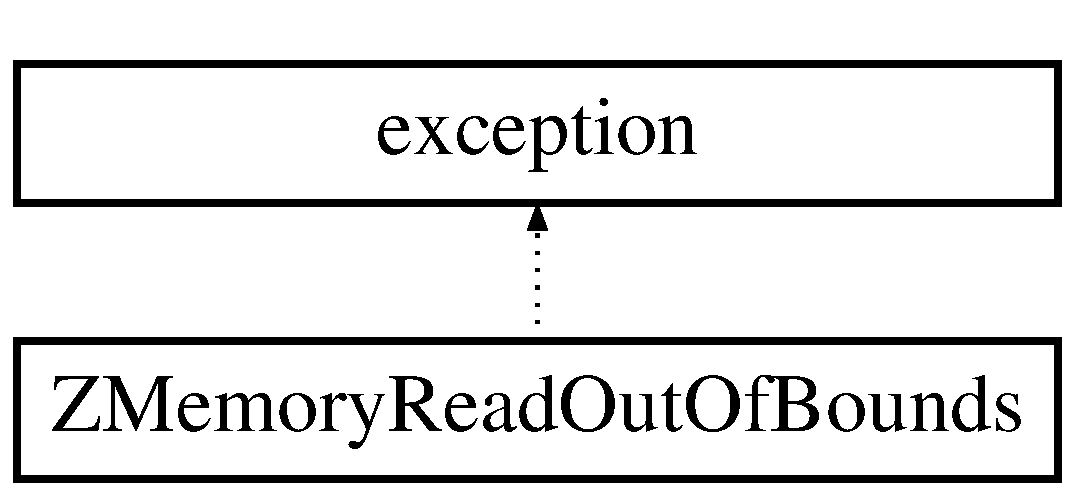
\includegraphics[height=2.000000cm]{class_z_memory_read_out_of_bounds}
\end{center}
\end{figure}
\subsection*{Public Member Functions}
\begin{DoxyCompactItemize}
\item 
\hyperlink{class_z_memory_read_out_of_bounds_a92ffa367d6036e39011b371cad3b9925}{Z\-Memory\-Read\-Out\-Of\-Bounds} ()
\end{DoxyCompactItemize}


\subsection{Constructor \& Destructor Documentation}
\hypertarget{class_z_memory_read_out_of_bounds_a92ffa367d6036e39011b371cad3b9925}{\index{Z\-Memory\-Read\-Out\-Of\-Bounds@{Z\-Memory\-Read\-Out\-Of\-Bounds}!Z\-Memory\-Read\-Out\-Of\-Bounds@{Z\-Memory\-Read\-Out\-Of\-Bounds}}
\index{Z\-Memory\-Read\-Out\-Of\-Bounds@{Z\-Memory\-Read\-Out\-Of\-Bounds}!ZMemoryReadOutOfBounds@{Z\-Memory\-Read\-Out\-Of\-Bounds}}
\subsubsection[{Z\-Memory\-Read\-Out\-Of\-Bounds}]{\setlength{\rightskip}{0pt plus 5cm}Z\-Memory\-Read\-Out\-Of\-Bounds\-::\-Z\-Memory\-Read\-Out\-Of\-Bounds (
\begin{DoxyParamCaption}
{}
\end{DoxyParamCaption}
)\hspace{0.3cm}{\ttfamily [inline]}}}\label{class_z_memory_read_out_of_bounds_a92ffa367d6036e39011b371cad3b9925}


The documentation for this class was generated from the following file\-:\begin{DoxyCompactItemize}
\item 
H\-:/code/c++/zebra-\/zmachine-\/interpreter/zmemory/zmemory/\hyperlink{zmemory_8h}{zmemory.\-h}\end{DoxyCompactItemize}

\hypertarget{class_z_memory_write_out_of_bounds}{\section{Z\-Memory\-Write\-Out\-Of\-Bounds Class Reference}
\label{class_z_memory_write_out_of_bounds}\index{Z\-Memory\-Write\-Out\-Of\-Bounds@{Z\-Memory\-Write\-Out\-Of\-Bounds}}
}


{\ttfamily \#include $<$zmemory.\-h$>$}

Inheritance diagram for Z\-Memory\-Write\-Out\-Of\-Bounds\-:\begin{figure}[H]
\begin{center}
\leavevmode
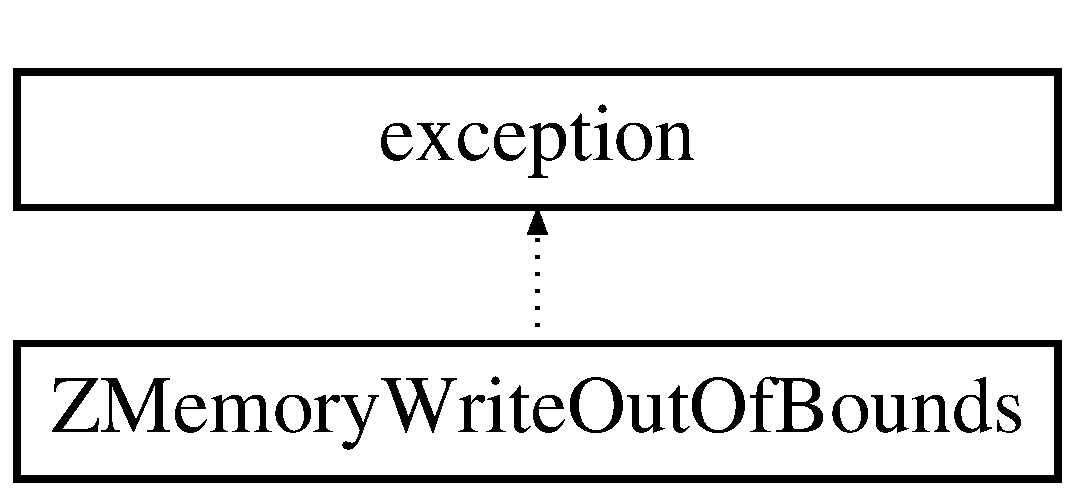
\includegraphics[height=2.000000cm]{class_z_memory_write_out_of_bounds}
\end{center}
\end{figure}
\subsection*{Public Member Functions}
\begin{DoxyCompactItemize}
\item 
\hyperlink{class_z_memory_write_out_of_bounds_a1e6d716a4f6209d43fe3953c9b348af3}{Z\-Memory\-Write\-Out\-Of\-Bounds} ()
\end{DoxyCompactItemize}


\subsection{Constructor \& Destructor Documentation}
\hypertarget{class_z_memory_write_out_of_bounds_a1e6d716a4f6209d43fe3953c9b348af3}{\index{Z\-Memory\-Write\-Out\-Of\-Bounds@{Z\-Memory\-Write\-Out\-Of\-Bounds}!Z\-Memory\-Write\-Out\-Of\-Bounds@{Z\-Memory\-Write\-Out\-Of\-Bounds}}
\index{Z\-Memory\-Write\-Out\-Of\-Bounds@{Z\-Memory\-Write\-Out\-Of\-Bounds}!ZMemoryWriteOutOfBounds@{Z\-Memory\-Write\-Out\-Of\-Bounds}}
\subsubsection[{Z\-Memory\-Write\-Out\-Of\-Bounds}]{\setlength{\rightskip}{0pt plus 5cm}Z\-Memory\-Write\-Out\-Of\-Bounds\-::\-Z\-Memory\-Write\-Out\-Of\-Bounds (
\begin{DoxyParamCaption}
{}
\end{DoxyParamCaption}
)\hspace{0.3cm}{\ttfamily [inline]}}}\label{class_z_memory_write_out_of_bounds_a1e6d716a4f6209d43fe3953c9b348af3}


The documentation for this class was generated from the following file\-:\begin{DoxyCompactItemize}
\item 
H\-:/code/c++/zebra-\/zmachine-\/interpreter/zmemory/zmemory/\hyperlink{zmemory_8h}{zmemory.\-h}\end{DoxyCompactItemize}

\hypertarget{class_z_object_table}{\section{Z\-Object\-Table Class Reference}
\label{class_z_object_table}\index{Z\-Object\-Table@{Z\-Object\-Table}}
}


{\ttfamily \#include $<$zobject.\-h$>$}

\subsection*{Public Member Functions}
\begin{DoxyCompactItemize}
\item 
\hyperlink{class_z_object_table_ad36c6a652bffa45d8c5217eb2fbe1e84}{Z\-Object\-Table} ()
\item 
\hyperlink{class_z_object_table_a7de1cb9995571422e98bf68bb8b37f65}{Z\-Object\-Table} (\hyperlink{class_z_memory}{Z\-Memory} $\ast$z\-Mem\-Obj)
\item 
\hyperlink{class_z_object_table_aec7ef9a6dfa851223fd546dd3b083c43}{$\sim$\-Z\-Object\-Table} ()
\item 
\hyperlink{zglobal_8h_a718b4eb2652c286f4d42dc18a8e71a1a}{ulong} \hyperlink{class_z_object_table_a0891575083b39a4d776b145ab21c4d7d}{get\-Object\-Addr} (\hyperlink{zglobal_8h_a718b4eb2652c286f4d42dc18a8e71a1a}{ulong} index)  throw (\-Illegal\-Object\-Index)
\item 
\hyperlink{zglobal_8h_a6507dc55d18847442d5fb20b6c73fe73}{zword} \hyperlink{class_z_object_table_aa9f8ea6a93111ecf70b7591cba14b03e}{get\-Default\-Property} (\hyperlink{zglobal_8h_a718b4eb2652c286f4d42dc18a8e71a1a}{ulong} index)  throw (\-Illegal\-Property\-Index)
\item 
\hyperlink{zglobal_8h_a718b4eb2652c286f4d42dc18a8e71a1a}{ulong} \hyperlink{class_z_object_table_abce2d0d913ce0111458c7087471c3510}{get\-Object\-Attribute\-Flags32} (\hyperlink{zglobal_8h_a718b4eb2652c286f4d42dc18a8e71a1a}{ulong} index)  throw (\-Illegal\-Object\-Index)
\item 
\hyperlink{zglobal_8h_a718b4eb2652c286f4d42dc18a8e71a1a}{ulong} \hyperlink{class_z_object_table_af0cbd1dc351eae1f789c3354eade9cb0}{get\-Object\-Attribute\-Flags48} (\hyperlink{zglobal_8h_a718b4eb2652c286f4d42dc18a8e71a1a}{ulong} index)  throw (\-Illegal\-Object\-Index)
\item 
\hyperlink{zglobal_8h_a6507dc55d18847442d5fb20b6c73fe73}{zword} \hyperlink{class_z_object_table_aabcd247354045552f410a6ba69501f6f}{get\-Object\-Parent} (\hyperlink{zglobal_8h_a718b4eb2652c286f4d42dc18a8e71a1a}{ulong} index)  throw (\-Illegal\-Object\-Index)
\item 
\hyperlink{zglobal_8h_a6507dc55d18847442d5fb20b6c73fe73}{zword} \hyperlink{class_z_object_table_a7c8e7d37438dd344ec0bb79de81eae13}{get\-Object\-Sibling} (\hyperlink{zglobal_8h_a718b4eb2652c286f4d42dc18a8e71a1a}{ulong} index)  throw (\-Illegal\-Object\-Index)
\item 
\hyperlink{zglobal_8h_a6507dc55d18847442d5fb20b6c73fe73}{zword} \hyperlink{class_z_object_table_abfbb91b1aac42c31e3f3b6f6be1dec43}{get\-Object\-Child} (\hyperlink{zglobal_8h_a718b4eb2652c286f4d42dc18a8e71a1a}{ulong} index)  throw (\-Illegal\-Object\-Index)
\item 
\hyperlink{zglobal_8h_a6507dc55d18847442d5fb20b6c73fe73}{zword} \hyperlink{class_z_object_table_adbad0758374585df5a515b453ced3730}{get\-Object\-Property\-List\-Addr} (\hyperlink{zglobal_8h_a718b4eb2652c286f4d42dc18a8e71a1a}{ulong} index)  throw (\-Illegal\-Object\-Index)
\item 
\hyperlink{zglobal_8h_a6507dc55d18847442d5fb20b6c73fe73}{zword} \hyperlink{class_z_object_table_a4811f880ec7c8853a008ef0911a5d8d0}{get\-Object\-Property\-Header\-Addr} (\hyperlink{zglobal_8h_a718b4eb2652c286f4d42dc18a8e71a1a}{ulong} index)  throw (\-Illegal\-Object\-Index)
\item 
\hyperlink{zglobal_8h_a6507dc55d18847442d5fb20b6c73fe73}{zword} $\ast$ \hyperlink{class_z_object_table_a13a0cc1794155cfd2e5876736b4e76da}{get\-Object\-Name} (\hyperlink{zglobal_8h_a718b4eb2652c286f4d42dc18a8e71a1a}{ulong} index)  throw (\-Illegal\-Object\-Index)
\item 
\hyperlink{zglobal_8h_a6507dc55d18847442d5fb20b6c73fe73}{zword} \hyperlink{class_z_object_table_a2630e740f9e1f5ecbc49a3ed2ba92b8e}{set\-Object\-Parent} (\hyperlink{zglobal_8h_a718b4eb2652c286f4d42dc18a8e71a1a}{ulong} index\-Child, \hyperlink{zglobal_8h_a718b4eb2652c286f4d42dc18a8e71a1a}{ulong} index\-Parent)  throw (\-Illegal\-Object\-Index)
\item 
\hyperlink{zglobal_8h_a6507dc55d18847442d5fb20b6c73fe73}{zword} \hyperlink{class_z_object_table_adb004bf8381717c458cff4546e161a05}{set\-Object\-Sibling} (\hyperlink{zglobal_8h_a718b4eb2652c286f4d42dc18a8e71a1a}{ulong} index\-Object, \hyperlink{zglobal_8h_a718b4eb2652c286f4d42dc18a8e71a1a}{ulong} index\-Sibling)  throw (\-Illegal\-Object\-Index)
\item 
\hyperlink{zglobal_8h_a6507dc55d18847442d5fb20b6c73fe73}{zword} \hyperlink{class_z_object_table_a4100f0edd10768a8ecb9a3412c2e3d2b}{set\-Object\-Child} (\hyperlink{zglobal_8h_a718b4eb2652c286f4d42dc18a8e71a1a}{ulong} index\-Parent, \hyperlink{zglobal_8h_a718b4eb2652c286f4d42dc18a8e71a1a}{ulong} index\-Child)  throw (\-Illegal\-Object\-Index)
\item 
\hyperlink{zglobal_8h_a6507dc55d18847442d5fb20b6c73fe73}{zword} \hyperlink{class_z_object_table_ac2837bde69ea20e7b383e1095c12cf66}{get\-Property\-List\-Length} (\hyperlink{zglobal_8h_a6507dc55d18847442d5fb20b6c73fe73}{zword} addr)  throw (\-Z\-Memory\-Read\-Out\-Of\-Bounds)
\item 
\hyperlink{struct_object_property}{Object\-Property} \hyperlink{class_z_object_table_a0d810796dbe4db0baa4339df990914ab}{get\-Property\-List\-Elem} (\hyperlink{zglobal_8h_a6507dc55d18847442d5fb20b6c73fe73}{zword} addr, \hyperlink{zglobal_8h_a718b4eb2652c286f4d42dc18a8e71a1a}{ulong} index)  throw (\-Illegal\-Property\-Index)
\end{DoxyCompactItemize}


\subsection{Constructor \& Destructor Documentation}
\hypertarget{class_z_object_table_ad36c6a652bffa45d8c5217eb2fbe1e84}{\index{Z\-Object\-Table@{Z\-Object\-Table}!Z\-Object\-Table@{Z\-Object\-Table}}
\index{Z\-Object\-Table@{Z\-Object\-Table}!ZObjectTable@{Z\-Object\-Table}}
\subsubsection[{Z\-Object\-Table}]{\setlength{\rightskip}{0pt plus 5cm}Z\-Object\-Table\-::\-Z\-Object\-Table (
\begin{DoxyParamCaption}
{}
\end{DoxyParamCaption}
)}}\label{class_z_object_table_ad36c6a652bffa45d8c5217eb2fbe1e84}
\hypertarget{class_z_object_table_a7de1cb9995571422e98bf68bb8b37f65}{\index{Z\-Object\-Table@{Z\-Object\-Table}!Z\-Object\-Table@{Z\-Object\-Table}}
\index{Z\-Object\-Table@{Z\-Object\-Table}!ZObjectTable@{Z\-Object\-Table}}
\subsubsection[{Z\-Object\-Table}]{\setlength{\rightskip}{0pt plus 5cm}Z\-Object\-Table\-::\-Z\-Object\-Table (
\begin{DoxyParamCaption}
\item[{{\bf Z\-Memory} $\ast$}]{z\-Mem\-Obj}
\end{DoxyParamCaption}
)}}\label{class_z_object_table_a7de1cb9995571422e98bf68bb8b37f65}
\hypertarget{class_z_object_table_aec7ef9a6dfa851223fd546dd3b083c43}{\index{Z\-Object\-Table@{Z\-Object\-Table}!$\sim$\-Z\-Object\-Table@{$\sim$\-Z\-Object\-Table}}
\index{$\sim$\-Z\-Object\-Table@{$\sim$\-Z\-Object\-Table}!ZObjectTable@{Z\-Object\-Table}}
\subsubsection[{$\sim$\-Z\-Object\-Table}]{\setlength{\rightskip}{0pt plus 5cm}Z\-Object\-Table\-::$\sim$\-Z\-Object\-Table (
\begin{DoxyParamCaption}
{}
\end{DoxyParamCaption}
)}}\label{class_z_object_table_aec7ef9a6dfa851223fd546dd3b083c43}


\subsection{Member Function Documentation}
\hypertarget{class_z_object_table_aa9f8ea6a93111ecf70b7591cba14b03e}{\index{Z\-Object\-Table@{Z\-Object\-Table}!get\-Default\-Property@{get\-Default\-Property}}
\index{get\-Default\-Property@{get\-Default\-Property}!ZObjectTable@{Z\-Object\-Table}}
\subsubsection[{get\-Default\-Property}]{\setlength{\rightskip}{0pt plus 5cm}{\bf zword} Z\-Object\-Table\-::get\-Default\-Property (
\begin{DoxyParamCaption}
\item[{{\bf ulong}}]{index}
\end{DoxyParamCaption}
) throw  {\bf Illegal\-Property\-Index}) }}\label{class_z_object_table_aa9f8ea6a93111ecf70b7591cba14b03e}
\hypertarget{class_z_object_table_a0891575083b39a4d776b145ab21c4d7d}{\index{Z\-Object\-Table@{Z\-Object\-Table}!get\-Object\-Addr@{get\-Object\-Addr}}
\index{get\-Object\-Addr@{get\-Object\-Addr}!ZObjectTable@{Z\-Object\-Table}}
\subsubsection[{get\-Object\-Addr}]{\setlength{\rightskip}{0pt plus 5cm}{\bf ulong} Z\-Object\-Table\-::get\-Object\-Addr (
\begin{DoxyParamCaption}
\item[{{\bf ulong}}]{index}
\end{DoxyParamCaption}
) throw  {\bf Illegal\-Object\-Index}) }}\label{class_z_object_table_a0891575083b39a4d776b145ab21c4d7d}
\hypertarget{class_z_object_table_abce2d0d913ce0111458c7087471c3510}{\index{Z\-Object\-Table@{Z\-Object\-Table}!get\-Object\-Attribute\-Flags32@{get\-Object\-Attribute\-Flags32}}
\index{get\-Object\-Attribute\-Flags32@{get\-Object\-Attribute\-Flags32}!ZObjectTable@{Z\-Object\-Table}}
\subsubsection[{get\-Object\-Attribute\-Flags32}]{\setlength{\rightskip}{0pt plus 5cm}{\bf ulong} Z\-Object\-Table\-::get\-Object\-Attribute\-Flags32 (
\begin{DoxyParamCaption}
\item[{{\bf ulong}}]{index}
\end{DoxyParamCaption}
) throw  {\bf Illegal\-Object\-Index}) }}\label{class_z_object_table_abce2d0d913ce0111458c7087471c3510}
\hypertarget{class_z_object_table_af0cbd1dc351eae1f789c3354eade9cb0}{\index{Z\-Object\-Table@{Z\-Object\-Table}!get\-Object\-Attribute\-Flags48@{get\-Object\-Attribute\-Flags48}}
\index{get\-Object\-Attribute\-Flags48@{get\-Object\-Attribute\-Flags48}!ZObjectTable@{Z\-Object\-Table}}
\subsubsection[{get\-Object\-Attribute\-Flags48}]{\setlength{\rightskip}{0pt plus 5cm}{\bf ulong} Z\-Object\-Table\-::get\-Object\-Attribute\-Flags48 (
\begin{DoxyParamCaption}
\item[{{\bf ulong}}]{index}
\end{DoxyParamCaption}
) throw  {\bf Illegal\-Object\-Index}) }}\label{class_z_object_table_af0cbd1dc351eae1f789c3354eade9cb0}
\hypertarget{class_z_object_table_abfbb91b1aac42c31e3f3b6f6be1dec43}{\index{Z\-Object\-Table@{Z\-Object\-Table}!get\-Object\-Child@{get\-Object\-Child}}
\index{get\-Object\-Child@{get\-Object\-Child}!ZObjectTable@{Z\-Object\-Table}}
\subsubsection[{get\-Object\-Child}]{\setlength{\rightskip}{0pt plus 5cm}{\bf zword} Z\-Object\-Table\-::get\-Object\-Child (
\begin{DoxyParamCaption}
\item[{{\bf ulong}}]{index}
\end{DoxyParamCaption}
) throw  {\bf Illegal\-Object\-Index}) }}\label{class_z_object_table_abfbb91b1aac42c31e3f3b6f6be1dec43}
\hypertarget{class_z_object_table_a13a0cc1794155cfd2e5876736b4e76da}{\index{Z\-Object\-Table@{Z\-Object\-Table}!get\-Object\-Name@{get\-Object\-Name}}
\index{get\-Object\-Name@{get\-Object\-Name}!ZObjectTable@{Z\-Object\-Table}}
\subsubsection[{get\-Object\-Name}]{\setlength{\rightskip}{0pt plus 5cm}{\bf zword} $\ast$ Z\-Object\-Table\-::get\-Object\-Name (
\begin{DoxyParamCaption}
\item[{{\bf ulong}}]{index}
\end{DoxyParamCaption}
) throw  {\bf Illegal\-Object\-Index}) }}\label{class_z_object_table_a13a0cc1794155cfd2e5876736b4e76da}
\hypertarget{class_z_object_table_aabcd247354045552f410a6ba69501f6f}{\index{Z\-Object\-Table@{Z\-Object\-Table}!get\-Object\-Parent@{get\-Object\-Parent}}
\index{get\-Object\-Parent@{get\-Object\-Parent}!ZObjectTable@{Z\-Object\-Table}}
\subsubsection[{get\-Object\-Parent}]{\setlength{\rightskip}{0pt plus 5cm}{\bf zword} Z\-Object\-Table\-::get\-Object\-Parent (
\begin{DoxyParamCaption}
\item[{{\bf ulong}}]{index}
\end{DoxyParamCaption}
) throw  {\bf Illegal\-Object\-Index}) }}\label{class_z_object_table_aabcd247354045552f410a6ba69501f6f}
\hypertarget{class_z_object_table_a4811f880ec7c8853a008ef0911a5d8d0}{\index{Z\-Object\-Table@{Z\-Object\-Table}!get\-Object\-Property\-Header\-Addr@{get\-Object\-Property\-Header\-Addr}}
\index{get\-Object\-Property\-Header\-Addr@{get\-Object\-Property\-Header\-Addr}!ZObjectTable@{Z\-Object\-Table}}
\subsubsection[{get\-Object\-Property\-Header\-Addr}]{\setlength{\rightskip}{0pt plus 5cm}{\bf zword} Z\-Object\-Table\-::get\-Object\-Property\-Header\-Addr (
\begin{DoxyParamCaption}
\item[{{\bf ulong}}]{index}
\end{DoxyParamCaption}
) throw  {\bf Illegal\-Object\-Index}) }}\label{class_z_object_table_a4811f880ec7c8853a008ef0911a5d8d0}
\hypertarget{class_z_object_table_adbad0758374585df5a515b453ced3730}{\index{Z\-Object\-Table@{Z\-Object\-Table}!get\-Object\-Property\-List\-Addr@{get\-Object\-Property\-List\-Addr}}
\index{get\-Object\-Property\-List\-Addr@{get\-Object\-Property\-List\-Addr}!ZObjectTable@{Z\-Object\-Table}}
\subsubsection[{get\-Object\-Property\-List\-Addr}]{\setlength{\rightskip}{0pt plus 5cm}{\bf zword} Z\-Object\-Table\-::get\-Object\-Property\-List\-Addr (
\begin{DoxyParamCaption}
\item[{{\bf ulong}}]{index}
\end{DoxyParamCaption}
) throw  {\bf Illegal\-Object\-Index}) }}\label{class_z_object_table_adbad0758374585df5a515b453ced3730}
\hypertarget{class_z_object_table_a7c8e7d37438dd344ec0bb79de81eae13}{\index{Z\-Object\-Table@{Z\-Object\-Table}!get\-Object\-Sibling@{get\-Object\-Sibling}}
\index{get\-Object\-Sibling@{get\-Object\-Sibling}!ZObjectTable@{Z\-Object\-Table}}
\subsubsection[{get\-Object\-Sibling}]{\setlength{\rightskip}{0pt plus 5cm}{\bf zword} Z\-Object\-Table\-::get\-Object\-Sibling (
\begin{DoxyParamCaption}
\item[{{\bf ulong}}]{index}
\end{DoxyParamCaption}
) throw  {\bf Illegal\-Object\-Index}) }}\label{class_z_object_table_a7c8e7d37438dd344ec0bb79de81eae13}
\hypertarget{class_z_object_table_a0d810796dbe4db0baa4339df990914ab}{\index{Z\-Object\-Table@{Z\-Object\-Table}!get\-Property\-List\-Elem@{get\-Property\-List\-Elem}}
\index{get\-Property\-List\-Elem@{get\-Property\-List\-Elem}!ZObjectTable@{Z\-Object\-Table}}
\subsubsection[{get\-Property\-List\-Elem}]{\setlength{\rightskip}{0pt plus 5cm}{\bf Object\-Property} Z\-Object\-Table\-::get\-Property\-List\-Elem (
\begin{DoxyParamCaption}
\item[{{\bf zword}}]{addr, }
\item[{{\bf ulong}}]{index}
\end{DoxyParamCaption}
) throw  {\bf Illegal\-Property\-Index}) }}\label{class_z_object_table_a0d810796dbe4db0baa4339df990914ab}
\hypertarget{class_z_object_table_ac2837bde69ea20e7b383e1095c12cf66}{\index{Z\-Object\-Table@{Z\-Object\-Table}!get\-Property\-List\-Length@{get\-Property\-List\-Length}}
\index{get\-Property\-List\-Length@{get\-Property\-List\-Length}!ZObjectTable@{Z\-Object\-Table}}
\subsubsection[{get\-Property\-List\-Length}]{\setlength{\rightskip}{0pt plus 5cm}{\bf zword} Z\-Object\-Table\-::get\-Property\-List\-Length (
\begin{DoxyParamCaption}
\item[{{\bf zword}}]{addr}
\end{DoxyParamCaption}
) throw  {\bf Z\-Memory\-Read\-Out\-Of\-Bounds}) }}\label{class_z_object_table_ac2837bde69ea20e7b383e1095c12cf66}
\hypertarget{class_z_object_table_a4100f0edd10768a8ecb9a3412c2e3d2b}{\index{Z\-Object\-Table@{Z\-Object\-Table}!set\-Object\-Child@{set\-Object\-Child}}
\index{set\-Object\-Child@{set\-Object\-Child}!ZObjectTable@{Z\-Object\-Table}}
\subsubsection[{set\-Object\-Child}]{\setlength{\rightskip}{0pt plus 5cm}{\bf zword} Z\-Object\-Table\-::set\-Object\-Child (
\begin{DoxyParamCaption}
\item[{{\bf ulong}}]{index\-Parent, }
\item[{{\bf ulong}}]{index\-Child}
\end{DoxyParamCaption}
) throw  {\bf Illegal\-Object\-Index}) }}\label{class_z_object_table_a4100f0edd10768a8ecb9a3412c2e3d2b}
\hypertarget{class_z_object_table_a2630e740f9e1f5ecbc49a3ed2ba92b8e}{\index{Z\-Object\-Table@{Z\-Object\-Table}!set\-Object\-Parent@{set\-Object\-Parent}}
\index{set\-Object\-Parent@{set\-Object\-Parent}!ZObjectTable@{Z\-Object\-Table}}
\subsubsection[{set\-Object\-Parent}]{\setlength{\rightskip}{0pt plus 5cm}{\bf zword} Z\-Object\-Table\-::set\-Object\-Parent (
\begin{DoxyParamCaption}
\item[{{\bf ulong}}]{index\-Child, }
\item[{{\bf ulong}}]{index\-Parent}
\end{DoxyParamCaption}
) throw  {\bf Illegal\-Object\-Index}) }}\label{class_z_object_table_a2630e740f9e1f5ecbc49a3ed2ba92b8e}
\hypertarget{class_z_object_table_adb004bf8381717c458cff4546e161a05}{\index{Z\-Object\-Table@{Z\-Object\-Table}!set\-Object\-Sibling@{set\-Object\-Sibling}}
\index{set\-Object\-Sibling@{set\-Object\-Sibling}!ZObjectTable@{Z\-Object\-Table}}
\subsubsection[{set\-Object\-Sibling}]{\setlength{\rightskip}{0pt plus 5cm}{\bf zword} Z\-Object\-Table\-::set\-Object\-Sibling (
\begin{DoxyParamCaption}
\item[{{\bf ulong}}]{index\-Object, }
\item[{{\bf ulong}}]{index\-Sibling}
\end{DoxyParamCaption}
) throw  {\bf Illegal\-Object\-Index}) }}\label{class_z_object_table_adb004bf8381717c458cff4546e161a05}


The documentation for this class was generated from the following files\-:\begin{DoxyCompactItemize}
\item 
H\-:/code/c++/zebra-\/zmachine-\/interpreter/zmemory/zmemory/\hyperlink{zobject_8h}{zobject.\-h}\item 
H\-:/code/c++/zebra-\/zmachine-\/interpreter/zmemory/zmemory/\hyperlink{zobject_8cpp}{zobject.\-cpp}\end{DoxyCompactItemize}

\hypertarget{class_z_stack}{\section{Z\-Stack Class Reference}
\label{class_z_stack}\index{Z\-Stack@{Z\-Stack}}
}


{\ttfamily \#include $<$zstack.\-h$>$}

\subsection*{Public Member Functions}
\begin{DoxyCompactItemize}
\item 
\hyperlink{class_z_stack_a409c413ad7d0337b57cd31a592c645a5}{Z\-Stack} ()
\item 
\hyperlink{class_z_stack_a05315db9ec1a92ae6bf3fac4b6461aa2}{$\sim$\-Z\-Stack} ()
\item 
bool \hyperlink{class_z_stack_aeacbf26a8e1ddc06d743bf0bf4332c2c}{is\-Stack\-Empty} ()
\item 
bool \hyperlink{class_z_stack_a2c753bb7460754603382b7f2dc90f108}{init\-Stack} (int size)
\item 
void \hyperlink{class_z_stack_a8dd1bb5131357ed8be9335eeb01b2fdb}{push} (\hyperlink{zglobal_8h_a6507dc55d18847442d5fb20b6c73fe73}{zword} val)  throw (\-Stack\-Full\-Exception)
\item 
\hyperlink{zglobal_8h_a6507dc55d18847442d5fb20b6c73fe73}{zword} \hyperlink{class_z_stack_a5c821f5c9a20f039774faecffb39697c}{pull} ()  throw (\-Stack\-Empty\-Exception)
\end{DoxyCompactItemize}


\subsection{Constructor \& Destructor Documentation}
\hypertarget{class_z_stack_a409c413ad7d0337b57cd31a592c645a5}{\index{Z\-Stack@{Z\-Stack}!Z\-Stack@{Z\-Stack}}
\index{Z\-Stack@{Z\-Stack}!ZStack@{Z\-Stack}}
\subsubsection[{Z\-Stack}]{\setlength{\rightskip}{0pt plus 5cm}Z\-Stack\-::\-Z\-Stack (
\begin{DoxyParamCaption}
{}
\end{DoxyParamCaption}
)}}\label{class_z_stack_a409c413ad7d0337b57cd31a592c645a5}
\hypertarget{class_z_stack_a05315db9ec1a92ae6bf3fac4b6461aa2}{\index{Z\-Stack@{Z\-Stack}!$\sim$\-Z\-Stack@{$\sim$\-Z\-Stack}}
\index{$\sim$\-Z\-Stack@{$\sim$\-Z\-Stack}!ZStack@{Z\-Stack}}
\subsubsection[{$\sim$\-Z\-Stack}]{\setlength{\rightskip}{0pt plus 5cm}Z\-Stack\-::$\sim$\-Z\-Stack (
\begin{DoxyParamCaption}
{}
\end{DoxyParamCaption}
)}}\label{class_z_stack_a05315db9ec1a92ae6bf3fac4b6461aa2}


\subsection{Member Function Documentation}
\hypertarget{class_z_stack_a2c753bb7460754603382b7f2dc90f108}{\index{Z\-Stack@{Z\-Stack}!init\-Stack@{init\-Stack}}
\index{init\-Stack@{init\-Stack}!ZStack@{Z\-Stack}}
\subsubsection[{init\-Stack}]{\setlength{\rightskip}{0pt plus 5cm}bool Z\-Stack\-::init\-Stack (
\begin{DoxyParamCaption}
\item[{int}]{size}
\end{DoxyParamCaption}
)}}\label{class_z_stack_a2c753bb7460754603382b7f2dc90f108}
\hypertarget{class_z_stack_aeacbf26a8e1ddc06d743bf0bf4332c2c}{\index{Z\-Stack@{Z\-Stack}!is\-Stack\-Empty@{is\-Stack\-Empty}}
\index{is\-Stack\-Empty@{is\-Stack\-Empty}!ZStack@{Z\-Stack}}
\subsubsection[{is\-Stack\-Empty}]{\setlength{\rightskip}{0pt plus 5cm}bool Z\-Stack\-::is\-Stack\-Empty (
\begin{DoxyParamCaption}
{}
\end{DoxyParamCaption}
)}}\label{class_z_stack_aeacbf26a8e1ddc06d743bf0bf4332c2c}
\hypertarget{class_z_stack_a5c821f5c9a20f039774faecffb39697c}{\index{Z\-Stack@{Z\-Stack}!pull@{pull}}
\index{pull@{pull}!ZStack@{Z\-Stack}}
\subsubsection[{pull}]{\setlength{\rightskip}{0pt plus 5cm}{\bf zword} Z\-Stack\-::pull (
\begin{DoxyParamCaption}
{}
\end{DoxyParamCaption}
) throw  {\bf Stack\-Empty\-Exception}) }}\label{class_z_stack_a5c821f5c9a20f039774faecffb39697c}
\hypertarget{class_z_stack_a8dd1bb5131357ed8be9335eeb01b2fdb}{\index{Z\-Stack@{Z\-Stack}!push@{push}}
\index{push@{push}!ZStack@{Z\-Stack}}
\subsubsection[{push}]{\setlength{\rightskip}{0pt plus 5cm}void Z\-Stack\-::push (
\begin{DoxyParamCaption}
\item[{{\bf zword}}]{val}
\end{DoxyParamCaption}
) throw  {\bf Stack\-Full\-Exception}) }}\label{class_z_stack_a8dd1bb5131357ed8be9335eeb01b2fdb}


The documentation for this class was generated from the following files\-:\begin{DoxyCompactItemize}
\item 
H\-:/code/c++/zebra-\/zmachine-\/interpreter/zstack/zstack/\hyperlink{zstack_8h}{zstack.\-h}\item 
H\-:/code/c++/zebra-\/zmachine-\/interpreter/zstack/zstack/\hyperlink{zstack_8cpp}{zstack.\-cpp}\end{DoxyCompactItemize}

\chapter{File Documentation}
\hypertarget{zdictionary_2zdictionary_2main_8cpp}{\section{H\-:/code/c++/zebra-\/zmachine-\/interpreter/zdictionary/zdictionary/main.cpp File Reference}
\label{zdictionary_2zdictionary_2main_8cpp}\index{H\-:/code/c++/zebra-\/zmachine-\/interpreter/zdictionary/zdictionary/main.\-cpp@{H\-:/code/c++/zebra-\/zmachine-\/interpreter/zdictionary/zdictionary/main.\-cpp}}
}
{\ttfamily \#include $<$iostream$>$}\\*
{\ttfamily \#include $<$cstdio$>$}\\*
{\ttfamily \#include \char`\"{}zdictionary.\-h\char`\"{}}\\*
{\ttfamily \#include \char`\"{}../../zglobal/zglobal.\-h\char`\"{}}\\*
{\ttfamily \#include \char`\"{}../../ztext/ztext/ztext.\-h\char`\"{}}\\*
{\ttfamily \#include \char`\"{}../../zmemory/zmemory/zmemory.\-h\char`\"{}}\\*
{\ttfamily \#include \char`\"{}../../zmemory/zmemory/zobject.\-h\char`\"{}}\\*
{\ttfamily \#include \char`\"{}../../zerror/zerror/zerror.\-h\char`\"{}}\\*
\subsection*{Functions}
\begin{DoxyCompactItemize}
\item 
long \hyperlink{zdictionary_2zdictionary_2main_8cpp_a1867d6b5ef80d05d1462514b85de0a50}{filesize} (F\-I\-L\-E $\ast$stream)
\item 
int \hyperlink{zdictionary_2zdictionary_2main_8cpp_ae66f6b31b5ad750f1fe042a706a4e3d4}{main} ()
\end{DoxyCompactItemize}
\subsection*{Variables}
\begin{DoxyCompactItemize}
\item 
int \hyperlink{zdictionary_2zdictionary_2main_8cpp_a41df104fcf203bd399b170c36a3eca7d}{z\-Version}
\end{DoxyCompactItemize}


\subsection{Function Documentation}
\hypertarget{zdictionary_2zdictionary_2main_8cpp_a1867d6b5ef80d05d1462514b85de0a50}{\index{zdictionary/zdictionary/main.\-cpp@{zdictionary/zdictionary/main.\-cpp}!filesize@{filesize}}
\index{filesize@{filesize}!zdictionary/zdictionary/main.cpp@{zdictionary/zdictionary/main.\-cpp}}
\subsubsection[{filesize}]{\setlength{\rightskip}{0pt plus 5cm}long filesize (
\begin{DoxyParamCaption}
\item[{F\-I\-L\-E $\ast$}]{stream}
\end{DoxyParamCaption}
)}}\label{zdictionary_2zdictionary_2main_8cpp_a1867d6b5ef80d05d1462514b85de0a50}
\hypertarget{zdictionary_2zdictionary_2main_8cpp_ae66f6b31b5ad750f1fe042a706a4e3d4}{\index{zdictionary/zdictionary/main.\-cpp@{zdictionary/zdictionary/main.\-cpp}!main@{main}}
\index{main@{main}!zdictionary/zdictionary/main.cpp@{zdictionary/zdictionary/main.\-cpp}}
\subsubsection[{main}]{\setlength{\rightskip}{0pt plus 5cm}int main (
\begin{DoxyParamCaption}
{}
\end{DoxyParamCaption}
)}}\label{zdictionary_2zdictionary_2main_8cpp_ae66f6b31b5ad750f1fe042a706a4e3d4}


\subsection{Variable Documentation}
\hypertarget{zdictionary_2zdictionary_2main_8cpp_a41df104fcf203bd399b170c36a3eca7d}{\index{zdictionary/zdictionary/main.\-cpp@{zdictionary/zdictionary/main.\-cpp}!z\-Version@{z\-Version}}
\index{z\-Version@{z\-Version}!zdictionary/zdictionary/main.cpp@{zdictionary/zdictionary/main.\-cpp}}
\subsubsection[{z\-Version}]{\setlength{\rightskip}{0pt plus 5cm}int z\-Version}}\label{zdictionary_2zdictionary_2main_8cpp_a41df104fcf203bd399b170c36a3eca7d}

\hypertarget{zerror_2zerror_2main_8cpp}{\section{H\-:/code/c++/zebra-\/zmachine-\/interpreter/zerror/zerror/main.cpp File Reference}
\label{zerror_2zerror_2main_8cpp}\index{H\-:/code/c++/zebra-\/zmachine-\/interpreter/zerror/zerror/main.\-cpp@{H\-:/code/c++/zebra-\/zmachine-\/interpreter/zerror/zerror/main.\-cpp}}
}
{\ttfamily \#include $<$iostream$>$}\\*
\subsection*{Functions}
\begin{DoxyCompactItemize}
\item 
int \hyperlink{zerror_2zerror_2main_8cpp_ae66f6b31b5ad750f1fe042a706a4e3d4}{main} ()
\end{DoxyCompactItemize}


\subsection{Function Documentation}
\hypertarget{zerror_2zerror_2main_8cpp_ae66f6b31b5ad750f1fe042a706a4e3d4}{\index{zerror/zerror/main.\-cpp@{zerror/zerror/main.\-cpp}!main@{main}}
\index{main@{main}!zerror/zerror/main.cpp@{zerror/zerror/main.\-cpp}}
\subsubsection[{main}]{\setlength{\rightskip}{0pt plus 5cm}int main (
\begin{DoxyParamCaption}
{}
\end{DoxyParamCaption}
)}}\label{zerror_2zerror_2main_8cpp_ae66f6b31b5ad750f1fe042a706a4e3d4}

\hypertarget{zmemory_2zmemory_2main_8cpp}{\section{H\-:/code/c++/zebra-\/zmachine-\/interpreter/zmemory/zmemory/main.cpp File Reference}
\label{zmemory_2zmemory_2main_8cpp}\index{H\-:/code/c++/zebra-\/zmachine-\/interpreter/zmemory/zmemory/main.\-cpp@{H\-:/code/c++/zebra-\/zmachine-\/interpreter/zmemory/zmemory/main.\-cpp}}
}
{\ttfamily \#include $<$iostream$>$}\\*
{\ttfamily \#include $<$cstdio$>$}\\*
{\ttfamily \#include \char`\"{}zmemory.\-h\char`\"{}}\\*
{\ttfamily \#include \char`\"{}zobject.\-h\char`\"{}}\\*
{\ttfamily \#include \char`\"{}../../zerror/zerror/zerror.\-h\char`\"{}}\\*
{\ttfamily \#include \char`\"{}../../ztext/ztext/ztext.\-h\char`\"{}}\\*
\subsection*{Functions}
\begin{DoxyCompactItemize}
\item 
long \hyperlink{zmemory_2zmemory_2main_8cpp_a1867d6b5ef80d05d1462514b85de0a50}{filesize} (F\-I\-L\-E $\ast$stream)
\item 
int \hyperlink{zmemory_2zmemory_2main_8cpp_ae66f6b31b5ad750f1fe042a706a4e3d4}{main} ()
\end{DoxyCompactItemize}
\subsection*{Variables}
\begin{DoxyCompactItemize}
\item 
int \hyperlink{zmemory_2zmemory_2main_8cpp_a41df104fcf203bd399b170c36a3eca7d}{z\-Version}
\end{DoxyCompactItemize}


\subsection{Function Documentation}
\hypertarget{zmemory_2zmemory_2main_8cpp_a1867d6b5ef80d05d1462514b85de0a50}{\index{zmemory/zmemory/main.\-cpp@{zmemory/zmemory/main.\-cpp}!filesize@{filesize}}
\index{filesize@{filesize}!zmemory/zmemory/main.cpp@{zmemory/zmemory/main.\-cpp}}
\subsubsection[{filesize}]{\setlength{\rightskip}{0pt plus 5cm}long filesize (
\begin{DoxyParamCaption}
\item[{F\-I\-L\-E $\ast$}]{stream}
\end{DoxyParamCaption}
)}}\label{zmemory_2zmemory_2main_8cpp_a1867d6b5ef80d05d1462514b85de0a50}
\hypertarget{zmemory_2zmemory_2main_8cpp_ae66f6b31b5ad750f1fe042a706a4e3d4}{\index{zmemory/zmemory/main.\-cpp@{zmemory/zmemory/main.\-cpp}!main@{main}}
\index{main@{main}!zmemory/zmemory/main.cpp@{zmemory/zmemory/main.\-cpp}}
\subsubsection[{main}]{\setlength{\rightskip}{0pt plus 5cm}int main (
\begin{DoxyParamCaption}
{}
\end{DoxyParamCaption}
)}}\label{zmemory_2zmemory_2main_8cpp_ae66f6b31b5ad750f1fe042a706a4e3d4}


\subsection{Variable Documentation}
\hypertarget{zmemory_2zmemory_2main_8cpp_a41df104fcf203bd399b170c36a3eca7d}{\index{zmemory/zmemory/main.\-cpp@{zmemory/zmemory/main.\-cpp}!z\-Version@{z\-Version}}
\index{z\-Version@{z\-Version}!zmemory/zmemory/main.cpp@{zmemory/zmemory/main.\-cpp}}
\subsubsection[{z\-Version}]{\setlength{\rightskip}{0pt plus 5cm}int z\-Version}}\label{zmemory_2zmemory_2main_8cpp_a41df104fcf203bd399b170c36a3eca7d}

\hypertarget{zstack_2zstack_2main_8cpp}{\section{H\-:/code/c++/zebra-\/zmachine-\/interpreter/zstack/zstack/main.cpp File Reference}
\label{zstack_2zstack_2main_8cpp}\index{H\-:/code/c++/zebra-\/zmachine-\/interpreter/zstack/zstack/main.\-cpp@{H\-:/code/c++/zebra-\/zmachine-\/interpreter/zstack/zstack/main.\-cpp}}
}
{\ttfamily \#include $<$iostream$>$}\\*
{\ttfamily \#include \char`\"{}zstack.\-h\char`\"{}}\\*
{\ttfamily \#include \char`\"{}conio.\-h\char`\"{}}\\*
{\ttfamily \#include \char`\"{}..\textbackslash{}..\textbackslash{}zglobal\textbackslash{}zglobal.\-h\char`\"{}}\\*
\subsection*{Functions}
\begin{DoxyCompactItemize}
\item 
int \hyperlink{zstack_2zstack_2main_8cpp_ae66f6b31b5ad750f1fe042a706a4e3d4}{main} ()
\end{DoxyCompactItemize}


\subsection{Function Documentation}
\hypertarget{zstack_2zstack_2main_8cpp_ae66f6b31b5ad750f1fe042a706a4e3d4}{\index{zstack/zstack/main.\-cpp@{zstack/zstack/main.\-cpp}!main@{main}}
\index{main@{main}!zstack/zstack/main.cpp@{zstack/zstack/main.\-cpp}}
\subsubsection[{main}]{\setlength{\rightskip}{0pt plus 5cm}int main (
\begin{DoxyParamCaption}
{}
\end{DoxyParamCaption}
)}}\label{zstack_2zstack_2main_8cpp_ae66f6b31b5ad750f1fe042a706a4e3d4}

\hypertarget{ztext_2ztext_2main_8cpp}{\section{H\-:/code/c++/zebra-\/zmachine-\/interpreter/ztext/ztext/main.cpp File Reference}
\label{ztext_2ztext_2main_8cpp}\index{H\-:/code/c++/zebra-\/zmachine-\/interpreter/ztext/ztext/main.\-cpp@{H\-:/code/c++/zebra-\/zmachine-\/interpreter/ztext/ztext/main.\-cpp}}
}
{\ttfamily \#include $<$iostream$>$}\\*
{\ttfamily \#include $<$cstdio$>$}\\*
{\ttfamily \#include \char`\"{}../../zmemory/zmemory/zmemory.\-h\char`\"{}}\\*
{\ttfamily \#include \char`\"{}../../zmemory/zmemory/zobject.\-h\char`\"{}}\\*
{\ttfamily \#include \char`\"{}../../zerror/zerror/zerror.\-h\char`\"{}}\\*
{\ttfamily \#include \char`\"{}ztext.\-h\char`\"{}}\\*
{\ttfamily \#include $<$conio.\-h$>$}\\*
{\ttfamily \#include $<$vector$>$}\\*
{\ttfamily \#include $<$exception$>$}\\*
\subsection*{Functions}
\begin{DoxyCompactItemize}
\item 
long \hyperlink{ztext_2ztext_2main_8cpp_a1867d6b5ef80d05d1462514b85de0a50}{filesize} (F\-I\-L\-E $\ast$stream)
\item 
int \hyperlink{ztext_2ztext_2main_8cpp_ae66f6b31b5ad750f1fe042a706a4e3d4}{main} ()
\end{DoxyCompactItemize}
\subsection*{Variables}
\begin{DoxyCompactItemize}
\item 
\hyperlink{zglobal_8h_aef68b14f6fcd84f18d5b177486e4999b}{zchar} \hyperlink{ztext_2ztext_2main_8cpp_ae991afe9cf5a78d591f33cce735aa9c7}{zstring} \mbox{[}11\mbox{]}
\item 
int \hyperlink{ztext_2ztext_2main_8cpp_a41df104fcf203bd399b170c36a3eca7d}{z\-Version}
\end{DoxyCompactItemize}


\subsection{Function Documentation}
\hypertarget{ztext_2ztext_2main_8cpp_a1867d6b5ef80d05d1462514b85de0a50}{\index{ztext/ztext/main.\-cpp@{ztext/ztext/main.\-cpp}!filesize@{filesize}}
\index{filesize@{filesize}!ztext/ztext/main.cpp@{ztext/ztext/main.\-cpp}}
\subsubsection[{filesize}]{\setlength{\rightskip}{0pt plus 5cm}long filesize (
\begin{DoxyParamCaption}
\item[{F\-I\-L\-E $\ast$}]{stream}
\end{DoxyParamCaption}
)}}\label{ztext_2ztext_2main_8cpp_a1867d6b5ef80d05d1462514b85de0a50}
\hypertarget{ztext_2ztext_2main_8cpp_ae66f6b31b5ad750f1fe042a706a4e3d4}{\index{ztext/ztext/main.\-cpp@{ztext/ztext/main.\-cpp}!main@{main}}
\index{main@{main}!ztext/ztext/main.cpp@{ztext/ztext/main.\-cpp}}
\subsubsection[{main}]{\setlength{\rightskip}{0pt plus 5cm}int main (
\begin{DoxyParamCaption}
{}
\end{DoxyParamCaption}
)}}\label{ztext_2ztext_2main_8cpp_ae66f6b31b5ad750f1fe042a706a4e3d4}


\subsection{Variable Documentation}
\hypertarget{ztext_2ztext_2main_8cpp_ae991afe9cf5a78d591f33cce735aa9c7}{\index{ztext/ztext/main.\-cpp@{ztext/ztext/main.\-cpp}!zstring@{zstring}}
\index{zstring@{zstring}!ztext/ztext/main.cpp@{ztext/ztext/main.\-cpp}}
\subsubsection[{zstring}]{\setlength{\rightskip}{0pt plus 5cm}{\bf zchar} zstring\mbox{[}11\mbox{]}}}\label{ztext_2ztext_2main_8cpp_ae991afe9cf5a78d591f33cce735aa9c7}
{\bfseries Initial value\-:}
\begin{DoxyCode}
= \{
    0x1F, 0x51, 0x31, 0xD3, 0x30, 0x08, 0x35, 0x58, 0xE4, 0xA5, 0x79
\}
\end{DoxyCode}
\hypertarget{ztext_2ztext_2main_8cpp_a41df104fcf203bd399b170c36a3eca7d}{\index{ztext/ztext/main.\-cpp@{ztext/ztext/main.\-cpp}!z\-Version@{z\-Version}}
\index{z\-Version@{z\-Version}!ztext/ztext/main.cpp@{ztext/ztext/main.\-cpp}}
\subsubsection[{z\-Version}]{\setlength{\rightskip}{0pt plus 5cm}int z\-Version}}\label{ztext_2ztext_2main_8cpp_a41df104fcf203bd399b170c36a3eca7d}

\hypertarget{zdictionary_8cpp}{\section{H\-:/code/c++/zebra-\/zmachine-\/interpreter/zdictionary/zdictionary/zdictionary.cpp File Reference}
\label{zdictionary_8cpp}\index{H\-:/code/c++/zebra-\/zmachine-\/interpreter/zdictionary/zdictionary/zdictionary.\-cpp@{H\-:/code/c++/zebra-\/zmachine-\/interpreter/zdictionary/zdictionary/zdictionary.\-cpp}}
}
{\ttfamily \#include \char`\"{}zdictionary.\-h\char`\"{}}\\*
{\ttfamily \#include $<$vector$>$}\\*
{\ttfamily \#include $<$string$>$}\\*
{\ttfamily \#include $<$cctype$>$}\\*

\hypertarget{zdictionary_8h}{\section{H\-:/code/c++/zebra-\/zmachine-\/interpreter/zdictionary/zdictionary/zdictionary.h File Reference}
\label{zdictionary_8h}\index{H\-:/code/c++/zebra-\/zmachine-\/interpreter/zdictionary/zdictionary/zdictionary.\-h@{H\-:/code/c++/zebra-\/zmachine-\/interpreter/zdictionary/zdictionary/zdictionary.\-h}}
}
{\ttfamily \#include $<$exception$>$}\\*
{\ttfamily \#include \char`\"{}../../zglobal/zglobal.\-h\char`\"{}}\\*
{\ttfamily \#include \char`\"{}../../zmemory/zmemory/zmemory.\-h\char`\"{}}\\*
{\ttfamily \#include \char`\"{}../../ztext/ztext/ztext.\-h\char`\"{}}\\*
\subsection*{Classes}
\begin{DoxyCompactItemize}
\item 
class \hyperlink{class_illegal_dictionary_index}{Illegal\-Dictionary\-Index}
\item 
struct \hyperlink{structz_dictionary_word}{z\-Dictionary\-Word}
\item 
class \hyperlink{class_z_dictionary}{Z\-Dictionary}
\end{DoxyCompactItemize}

\hypertarget{zerror_8cpp}{\section{H\-:/code/c++/zebra-\/zmachine-\/interpreter/zerror/zerror/zerror.cpp File Reference}
\label{zerror_8cpp}\index{H\-:/code/c++/zebra-\/zmachine-\/interpreter/zerror/zerror/zerror.\-cpp@{H\-:/code/c++/zebra-\/zmachine-\/interpreter/zerror/zerror/zerror.\-cpp}}
}
{\ttfamily \#include \char`\"{}zerror.\-h\char`\"{}}\\*
{\ttfamily \#include $<$cstdio$>$}\\*

\hypertarget{zerror_8h}{\section{H\-:/code/c++/zebra-\/zmachine-\/interpreter/zerror/zerror/zerror.h File Reference}
\label{zerror_8h}\index{H\-:/code/c++/zebra-\/zmachine-\/interpreter/zerror/zerror/zerror.\-h@{H\-:/code/c++/zebra-\/zmachine-\/interpreter/zerror/zerror/zerror.\-h}}
}
{\ttfamily \#include $<$string$>$}\\*
\subsection*{Classes}
\begin{DoxyCompactItemize}
\item 
class \hyperlink{class_z_error}{Z\-Error}
\end{DoxyCompactItemize}

\hypertarget{zglobal_8cpp}{\section{H\-:/code/c++/zebra-\/zmachine-\/interpreter/zglobal/zglobal.cpp File Reference}
\label{zglobal_8cpp}\index{H\-:/code/c++/zebra-\/zmachine-\/interpreter/zglobal/zglobal.\-cpp@{H\-:/code/c++/zebra-\/zmachine-\/interpreter/zglobal/zglobal.\-cpp}}
}
{\ttfamily \#include \char`\"{}zglobal.\-h\char`\"{}}\\*
{\ttfamily \#include $<$vector$>$}\\*
\subsection*{Functions}
\begin{DoxyCompactItemize}
\item 
\hyperlink{zglobal_8h_a6507dc55d18847442d5fb20b6c73fe73}{zword} \hyperlink{zglobal_8cpp_a6b53174cdd66beaefc6211c98da2eecd}{endianize} (\hyperlink{zglobal_8h_a6507dc55d18847442d5fb20b6c73fe73}{zword} in)
\item 
\hyperlink{zglobal_8h_a6507dc55d18847442d5fb20b6c73fe73}{zword} \hyperlink{zglobal_8cpp_a33ba994104fbf5c6ac8055ea96420623}{reverse\-Bit\-Sequence} (\hyperlink{zglobal_8h_aab4ef09707609e67bcc5a552cde255d2}{zbyte} in)
\end{DoxyCompactItemize}
\subsection*{Variables}
\begin{DoxyCompactItemize}
\item 
\hyperlink{class_z_error}{Z\-Error} \hyperlink{zglobal_8cpp_a14dd7c27cf5e3c6712ae1ab2ef444a9a}{z\-Error\-Logger}
\end{DoxyCompactItemize}


\subsection{Function Documentation}
\hypertarget{zglobal_8cpp_a6b53174cdd66beaefc6211c98da2eecd}{\index{zglobal.\-cpp@{zglobal.\-cpp}!endianize@{endianize}}
\index{endianize@{endianize}!zglobal.cpp@{zglobal.\-cpp}}
\subsubsection[{endianize}]{\setlength{\rightskip}{0pt plus 5cm}{\bf zword} endianize (
\begin{DoxyParamCaption}
\item[{{\bf zword}}]{in}
\end{DoxyParamCaption}
)}}\label{zglobal_8cpp_a6b53174cdd66beaefc6211c98da2eecd}
\hypertarget{zglobal_8cpp_a33ba994104fbf5c6ac8055ea96420623}{\index{zglobal.\-cpp@{zglobal.\-cpp}!reverse\-Bit\-Sequence@{reverse\-Bit\-Sequence}}
\index{reverse\-Bit\-Sequence@{reverse\-Bit\-Sequence}!zglobal.cpp@{zglobal.\-cpp}}
\subsubsection[{reverse\-Bit\-Sequence}]{\setlength{\rightskip}{0pt plus 5cm}{\bf zword} reverse\-Bit\-Sequence (
\begin{DoxyParamCaption}
\item[{{\bf zbyte}}]{in}
\end{DoxyParamCaption}
)}}\label{zglobal_8cpp_a33ba994104fbf5c6ac8055ea96420623}


\subsection{Variable Documentation}
\hypertarget{zglobal_8cpp_a14dd7c27cf5e3c6712ae1ab2ef444a9a}{\index{zglobal.\-cpp@{zglobal.\-cpp}!z\-Error\-Logger@{z\-Error\-Logger}}
\index{z\-Error\-Logger@{z\-Error\-Logger}!zglobal.cpp@{zglobal.\-cpp}}
\subsubsection[{z\-Error\-Logger}]{\setlength{\rightskip}{0pt plus 5cm}{\bf Z\-Error} z\-Error\-Logger}}\label{zglobal_8cpp_a14dd7c27cf5e3c6712ae1ab2ef444a9a}
\hyperlink{ztext_8h}{ztext.\-h} z-\/machine text functions 
\hypertarget{zglobal_8h}{\section{H\-:/code/c++/zebra-\/zmachine-\/interpreter/zglobal/zglobal.h File Reference}
\label{zglobal_8h}\index{H\-:/code/c++/zebra-\/zmachine-\/interpreter/zglobal/zglobal.\-h@{H\-:/code/c++/zebra-\/zmachine-\/interpreter/zglobal/zglobal.\-h}}
}
{\ttfamily \#include \char`\"{}../zerror/zerror/zerror.\-h\char`\"{}}\\*
{\ttfamily \#include $<$vector$>$}\\*
\subsection*{Typedefs}
\begin{DoxyCompactItemize}
\item 
typedef unsigned short \hyperlink{zglobal_8h_a6507dc55d18847442d5fb20b6c73fe73}{zword}
\item 
typedef unsigned char \hyperlink{zglobal_8h_aef68b14f6fcd84f18d5b177486e4999b}{zchar}
\item 
typedef unsigned char \hyperlink{zglobal_8h_aab4ef09707609e67bcc5a552cde255d2}{zbyte}
\item 
typedef unsigned long \hyperlink{zglobal_8h_a718b4eb2652c286f4d42dc18a8e71a1a}{ulong}
\end{DoxyCompactItemize}
\subsection*{Functions}
\begin{DoxyCompactItemize}
\item 
\hyperlink{zglobal_8h_a6507dc55d18847442d5fb20b6c73fe73}{zword} \hyperlink{zglobal_8h_a6b53174cdd66beaefc6211c98da2eecd}{endianize} (\hyperlink{zglobal_8h_a6507dc55d18847442d5fb20b6c73fe73}{zword} in)
\item 
\hyperlink{zglobal_8h_a6507dc55d18847442d5fb20b6c73fe73}{zword} \hyperlink{zglobal_8h_a33ba994104fbf5c6ac8055ea96420623}{reverse\-Bit\-Sequence} (\hyperlink{zglobal_8h_aab4ef09707609e67bcc5a552cde255d2}{zbyte} in)
\end{DoxyCompactItemize}


\subsection{Typedef Documentation}
\hypertarget{zglobal_8h_a718b4eb2652c286f4d42dc18a8e71a1a}{\index{zglobal.\-h@{zglobal.\-h}!ulong@{ulong}}
\index{ulong@{ulong}!zglobal.h@{zglobal.\-h}}
\subsubsection[{ulong}]{\setlength{\rightskip}{0pt plus 5cm}typedef unsigned long {\bf ulong}}}\label{zglobal_8h_a718b4eb2652c286f4d42dc18a8e71a1a}
\hypertarget{zglobal_8h_aab4ef09707609e67bcc5a552cde255d2}{\index{zglobal.\-h@{zglobal.\-h}!zbyte@{zbyte}}
\index{zbyte@{zbyte}!zglobal.h@{zglobal.\-h}}
\subsubsection[{zbyte}]{\setlength{\rightskip}{0pt plus 5cm}typedef unsigned char {\bf zbyte}}}\label{zglobal_8h_aab4ef09707609e67bcc5a552cde255d2}
\hypertarget{zglobal_8h_aef68b14f6fcd84f18d5b177486e4999b}{\index{zglobal.\-h@{zglobal.\-h}!zchar@{zchar}}
\index{zchar@{zchar}!zglobal.h@{zglobal.\-h}}
\subsubsection[{zchar}]{\setlength{\rightskip}{0pt plus 5cm}typedef unsigned char {\bf zchar}}}\label{zglobal_8h_aef68b14f6fcd84f18d5b177486e4999b}
\hypertarget{zglobal_8h_a6507dc55d18847442d5fb20b6c73fe73}{\index{zglobal.\-h@{zglobal.\-h}!zword@{zword}}
\index{zword@{zword}!zglobal.h@{zglobal.\-h}}
\subsubsection[{zword}]{\setlength{\rightskip}{0pt plus 5cm}typedef unsigned short {\bf zword}}}\label{zglobal_8h_a6507dc55d18847442d5fb20b6c73fe73}


\subsection{Function Documentation}
\hypertarget{zglobal_8h_a6b53174cdd66beaefc6211c98da2eecd}{\index{zglobal.\-h@{zglobal.\-h}!endianize@{endianize}}
\index{endianize@{endianize}!zglobal.h@{zglobal.\-h}}
\subsubsection[{endianize}]{\setlength{\rightskip}{0pt plus 5cm}{\bf zword} endianize (
\begin{DoxyParamCaption}
\item[{{\bf zword}}]{in}
\end{DoxyParamCaption}
)}}\label{zglobal_8h_a6b53174cdd66beaefc6211c98da2eecd}
\hypertarget{zglobal_8h_a33ba994104fbf5c6ac8055ea96420623}{\index{zglobal.\-h@{zglobal.\-h}!reverse\-Bit\-Sequence@{reverse\-Bit\-Sequence}}
\index{reverse\-Bit\-Sequence@{reverse\-Bit\-Sequence}!zglobal.h@{zglobal.\-h}}
\subsubsection[{reverse\-Bit\-Sequence}]{\setlength{\rightskip}{0pt plus 5cm}{\bf zword} reverse\-Bit\-Sequence (
\begin{DoxyParamCaption}
\item[{{\bf zbyte}}]{in}
\end{DoxyParamCaption}
)}}\label{zglobal_8h_a33ba994104fbf5c6ac8055ea96420623}

\hypertarget{zmemory_8cpp}{\section{H\-:/code/c++/zebra-\/zmachine-\/interpreter/zmemory/zmemory/zmemory.cpp File Reference}
\label{zmemory_8cpp}\index{H\-:/code/c++/zebra-\/zmachine-\/interpreter/zmemory/zmemory/zmemory.\-cpp@{H\-:/code/c++/zebra-\/zmachine-\/interpreter/zmemory/zmemory/zmemory.\-cpp}}
}
{\ttfamily \#include \char`\"{}zmemory.\-h\char`\"{}}\\*
{\ttfamily \#include \char`\"{}../../zglobal/zglobal.\-h\char`\"{}}\\*

\hypertarget{zmemory_8h}{\section{H\-:/code/c++/zebra-\/zmachine-\/interpreter/zmemory/zmemory/zmemory.h File Reference}
\label{zmemory_8h}\index{H\-:/code/c++/zebra-\/zmachine-\/interpreter/zmemory/zmemory/zmemory.\-h@{H\-:/code/c++/zebra-\/zmachine-\/interpreter/zmemory/zmemory/zmemory.\-h}}
}
{\ttfamily \#include \char`\"{}../../zglobal/zglobal.\-h\char`\"{}}\\*
{\ttfamily \#include \char`\"{}../../zerror/zerror/zerror.\-h\char`\"{}}\\*
{\ttfamily \#include $<$exception$>$}\\*
\subsection*{Classes}
\begin{DoxyCompactItemize}
\item 
class \hyperlink{class_z_memory_write_out_of_bounds}{Z\-Memory\-Write\-Out\-Of\-Bounds}
\item 
class \hyperlink{class_z_memory_read_out_of_bounds}{Z\-Memory\-Read\-Out\-Of\-Bounds}
\item 
class \hyperlink{class_z_memory}{Z\-Memory}
\end{DoxyCompactItemize}
\subsection*{Macros}
\begin{DoxyCompactItemize}
\item 
\#define \hyperlink{zmemory_8h_abe9c8211c3d460eb97e5b0997b8833fa}{Z\-M\-E\-M\-O\-R\-Y\-\_\-\-D\-Y\-N\-A\-M\-I\-C}~0
\item 
\#define \hyperlink{zmemory_8h_a4bd64bf64f0497628bc158a05a363c2e}{Z\-M\-E\-M\-O\-R\-Y\-\_\-\-S\-T\-A\-T\-I\-C}~1
\item 
\#define \hyperlink{zmemory_8h_acf07ee5a3f3daf8a0dddb4fe84e4b98f}{Z\-M\-E\-M\-O\-R\-Y\-\_\-\-H\-I\-G\-H}~2
\end{DoxyCompactItemize}
\subsection*{Variables}
\begin{DoxyCompactItemize}
\item 
int \hyperlink{zmemory_8h_a41df104fcf203bd399b170c36a3eca7d}{z\-Version}
\item 
\hyperlink{class_z_error}{Z\-Error} \hyperlink{zmemory_8h_a14dd7c27cf5e3c6712ae1ab2ef444a9a}{z\-Error\-Logger}
\end{DoxyCompactItemize}


\subsection{Macro Definition Documentation}
\hypertarget{zmemory_8h_abe9c8211c3d460eb97e5b0997b8833fa}{\index{zmemory.\-h@{zmemory.\-h}!Z\-M\-E\-M\-O\-R\-Y\-\_\-\-D\-Y\-N\-A\-M\-I\-C@{Z\-M\-E\-M\-O\-R\-Y\-\_\-\-D\-Y\-N\-A\-M\-I\-C}}
\index{Z\-M\-E\-M\-O\-R\-Y\-\_\-\-D\-Y\-N\-A\-M\-I\-C@{Z\-M\-E\-M\-O\-R\-Y\-\_\-\-D\-Y\-N\-A\-M\-I\-C}!zmemory.h@{zmemory.\-h}}
\subsubsection[{Z\-M\-E\-M\-O\-R\-Y\-\_\-\-D\-Y\-N\-A\-M\-I\-C}]{\setlength{\rightskip}{0pt plus 5cm}\#define Z\-M\-E\-M\-O\-R\-Y\-\_\-\-D\-Y\-N\-A\-M\-I\-C~0}}\label{zmemory_8h_abe9c8211c3d460eb97e5b0997b8833fa}
\hypertarget{zmemory_8h_acf07ee5a3f3daf8a0dddb4fe84e4b98f}{\index{zmemory.\-h@{zmemory.\-h}!Z\-M\-E\-M\-O\-R\-Y\-\_\-\-H\-I\-G\-H@{Z\-M\-E\-M\-O\-R\-Y\-\_\-\-H\-I\-G\-H}}
\index{Z\-M\-E\-M\-O\-R\-Y\-\_\-\-H\-I\-G\-H@{Z\-M\-E\-M\-O\-R\-Y\-\_\-\-H\-I\-G\-H}!zmemory.h@{zmemory.\-h}}
\subsubsection[{Z\-M\-E\-M\-O\-R\-Y\-\_\-\-H\-I\-G\-H}]{\setlength{\rightskip}{0pt plus 5cm}\#define Z\-M\-E\-M\-O\-R\-Y\-\_\-\-H\-I\-G\-H~2}}\label{zmemory_8h_acf07ee5a3f3daf8a0dddb4fe84e4b98f}
\hypertarget{zmemory_8h_a4bd64bf64f0497628bc158a05a363c2e}{\index{zmemory.\-h@{zmemory.\-h}!Z\-M\-E\-M\-O\-R\-Y\-\_\-\-S\-T\-A\-T\-I\-C@{Z\-M\-E\-M\-O\-R\-Y\-\_\-\-S\-T\-A\-T\-I\-C}}
\index{Z\-M\-E\-M\-O\-R\-Y\-\_\-\-S\-T\-A\-T\-I\-C@{Z\-M\-E\-M\-O\-R\-Y\-\_\-\-S\-T\-A\-T\-I\-C}!zmemory.h@{zmemory.\-h}}
\subsubsection[{Z\-M\-E\-M\-O\-R\-Y\-\_\-\-S\-T\-A\-T\-I\-C}]{\setlength{\rightskip}{0pt plus 5cm}\#define Z\-M\-E\-M\-O\-R\-Y\-\_\-\-S\-T\-A\-T\-I\-C~1}}\label{zmemory_8h_a4bd64bf64f0497628bc158a05a363c2e}


\subsection{Variable Documentation}
\hypertarget{zmemory_8h_a14dd7c27cf5e3c6712ae1ab2ef444a9a}{\index{zmemory.\-h@{zmemory.\-h}!z\-Error\-Logger@{z\-Error\-Logger}}
\index{z\-Error\-Logger@{z\-Error\-Logger}!zmemory.h@{zmemory.\-h}}
\subsubsection[{z\-Error\-Logger}]{\setlength{\rightskip}{0pt plus 5cm}{\bf Z\-Error} z\-Error\-Logger}}\label{zmemory_8h_a14dd7c27cf5e3c6712ae1ab2ef444a9a}
\hypertarget{zmemory_8h_a41df104fcf203bd399b170c36a3eca7d}{\index{zmemory.\-h@{zmemory.\-h}!z\-Version@{z\-Version}}
\index{z\-Version@{z\-Version}!zmemory.h@{zmemory.\-h}}
\subsubsection[{z\-Version}]{\setlength{\rightskip}{0pt plus 5cm}int z\-Version}}\label{zmemory_8h_a41df104fcf203bd399b170c36a3eca7d}

\hypertarget{zobject_8cpp}{\section{H\-:/code/c++/zebra-\/zmachine-\/interpreter/zmemory/zmemory/zobject.cpp File Reference}
\label{zobject_8cpp}\index{H\-:/code/c++/zebra-\/zmachine-\/interpreter/zmemory/zmemory/zobject.\-cpp@{H\-:/code/c++/zebra-\/zmachine-\/interpreter/zmemory/zmemory/zobject.\-cpp}}
}
{\ttfamily \#include \char`\"{}zobject.\-h\char`\"{}}\\*
\subsection*{Variables}
\begin{DoxyCompactItemize}
\item 
int \hyperlink{zobject_8cpp_a41df104fcf203bd399b170c36a3eca7d}{z\-Version}
\end{DoxyCompactItemize}


\subsection{Variable Documentation}
\hypertarget{zobject_8cpp_a41df104fcf203bd399b170c36a3eca7d}{\index{zobject.\-cpp@{zobject.\-cpp}!z\-Version@{z\-Version}}
\index{z\-Version@{z\-Version}!zobject.cpp@{zobject.\-cpp}}
\subsubsection[{z\-Version}]{\setlength{\rightskip}{0pt plus 5cm}int z\-Version}}\label{zobject_8cpp_a41df104fcf203bd399b170c36a3eca7d}

\hypertarget{zobject_8h}{\section{H\-:/code/c++/zebra-\/zmachine-\/interpreter/zmemory/zmemory/zobject.h File Reference}
\label{zobject_8h}\index{H\-:/code/c++/zebra-\/zmachine-\/interpreter/zmemory/zmemory/zobject.\-h@{H\-:/code/c++/zebra-\/zmachine-\/interpreter/zmemory/zmemory/zobject.\-h}}
}
{\ttfamily \#include \char`\"{}../../zglobal/zglobal.\-h\char`\"{}}\\*
{\ttfamily \#include \char`\"{}../../zerror/zerror/zerror.\-h\char`\"{}}\\*
{\ttfamily \#include \char`\"{}zmemory.\-h\char`\"{}}\\*
\subsection*{Classes}
\begin{DoxyCompactItemize}
\item 
class \hyperlink{class_illegal_object_index}{Illegal\-Object\-Index}
\item 
class \hyperlink{class_illegal_property_index}{Illegal\-Property\-Index}
\item 
struct \hyperlink{struct_object_property}{Object\-Property}
\item 
class \hyperlink{class_z_object_table}{Z\-Object\-Table}
\end{DoxyCompactItemize}
\subsection*{Variables}
\begin{DoxyCompactItemize}
\item 
int \hyperlink{zobject_8h_a41df104fcf203bd399b170c36a3eca7d}{z\-Version}
\item 
\hyperlink{class_z_error}{Z\-Error} \hyperlink{zobject_8h_a14dd7c27cf5e3c6712ae1ab2ef444a9a}{z\-Error\-Logger}
\end{DoxyCompactItemize}


\subsection{Variable Documentation}
\hypertarget{zobject_8h_a14dd7c27cf5e3c6712ae1ab2ef444a9a}{\index{zobject.\-h@{zobject.\-h}!z\-Error\-Logger@{z\-Error\-Logger}}
\index{z\-Error\-Logger@{z\-Error\-Logger}!zobject.h@{zobject.\-h}}
\subsubsection[{z\-Error\-Logger}]{\setlength{\rightskip}{0pt plus 5cm}{\bf Z\-Error} z\-Error\-Logger}}\label{zobject_8h_a14dd7c27cf5e3c6712ae1ab2ef444a9a}
\hypertarget{zobject_8h_a41df104fcf203bd399b170c36a3eca7d}{\index{zobject.\-h@{zobject.\-h}!z\-Version@{z\-Version}}
\index{z\-Version@{z\-Version}!zobject.h@{zobject.\-h}}
\subsubsection[{z\-Version}]{\setlength{\rightskip}{0pt plus 5cm}int z\-Version}}\label{zobject_8h_a41df104fcf203bd399b170c36a3eca7d}

\hypertarget{zstack_8cpp}{\section{H\-:/code/c++/zebra-\/zmachine-\/interpreter/zstack/zstack/zstack.cpp File Reference}
\label{zstack_8cpp}\index{H\-:/code/c++/zebra-\/zmachine-\/interpreter/zstack/zstack/zstack.\-cpp@{H\-:/code/c++/zebra-\/zmachine-\/interpreter/zstack/zstack/zstack.\-cpp}}
}
{\ttfamily \#include \char`\"{}zstack.\-h\char`\"{}}\\*
{\ttfamily \#include \char`\"{}..\textbackslash{}..\textbackslash{}zerror\textbackslash{}zerror\textbackslash{}zerror.\-h\char`\"{}}\\*

\hypertarget{zstack_8h}{\section{H\-:/code/c++/zebra-\/zmachine-\/interpreter/zstack/zstack/zstack.h File Reference}
\label{zstack_8h}\index{H\-:/code/c++/zebra-\/zmachine-\/interpreter/zstack/zstack/zstack.\-h@{H\-:/code/c++/zebra-\/zmachine-\/interpreter/zstack/zstack/zstack.\-h}}
}
{\ttfamily \#include $<$exception$>$}\\*
{\ttfamily \#include \char`\"{}..\textbackslash{}..\textbackslash{}zglobal\textbackslash{}zglobal.\-h\char`\"{}}\\*
\subsection*{Classes}
\begin{DoxyCompactItemize}
\item 
class \hyperlink{class_stack_empty_exception}{Stack\-Empty\-Exception}
\item 
class \hyperlink{class_stack_full_exception}{Stack\-Full\-Exception}
\item 
class \hyperlink{class_z_stack}{Z\-Stack}
\end{DoxyCompactItemize}

\hypertarget{ztext_8cpp}{\section{H\-:/code/c++/zebra-\/zmachine-\/interpreter/ztext/ztext/ztext.cpp File Reference}
\label{ztext_8cpp}\index{H\-:/code/c++/zebra-\/zmachine-\/interpreter/ztext/ztext/ztext.\-cpp@{H\-:/code/c++/zebra-\/zmachine-\/interpreter/ztext/ztext/ztext.\-cpp}}
}
{\ttfamily \#include \char`\"{}ztext.\-h\char`\"{}}\\*
{\ttfamily \#include \char`\"{}../../zmemory/zmemory/zmemory.\-h\char`\"{}}\\*
{\ttfamily \#include $<$vector$>$}\\*
\subsection*{Classes}
\begin{DoxyCompactItemize}
\item 
struct \hyperlink{structz_char_stringto_z_s_c_i_i_helper__save_state}{z\-Char\-Stringto\-Z\-S\-C\-I\-I\-Helper\-\_\-save\-State}
\end{DoxyCompactItemize}
\subsection*{Macros}
\begin{DoxyCompactItemize}
\item 
\#define \hyperlink{ztext_8cpp_a6ce196e7cdf5a09434c27e3304171754}{A\-L\-P\-H\-A\-B\-E\-T\-\_\-1}~1
\item 
\#define \hyperlink{ztext_8cpp_a9b2b2f2c7b68f470b7f9c2158c19b142}{A\-L\-P\-H\-A\-B\-E\-T\-\_\-2}~2
\item 
\#define \hyperlink{ztext_8cpp_af22148e65407494603b105d040e1da7c}{A\-L\-P\-H\-A\-B\-E\-T\-\_\-0}~0
\end{DoxyCompactItemize}
\subsection*{Functions}
\begin{DoxyCompactItemize}
\item 
int \hyperlink{ztext_8cpp_adbae7420748e6fc16b889ca69fe37d3e}{Z\-S\-C\-I\-I\-Str\-Len} (\hyperlink{zglobal_8h_aef68b14f6fcd84f18d5b177486e4999b}{zchar} $\ast$str)
\item 
int \hyperlink{ztext_8cpp_a47f99f33641c11c40bcaff032ab2bb07}{z\-Char\-Str\-Len} (\hyperlink{zglobal_8h_a6507dc55d18847442d5fb20b6c73fe73}{zword} $\ast$str)
\item 
void \hyperlink{ztext_8cpp_a1099a7a939f2758529062bceff394794}{Z\-S\-C\-I\-I\-Str\-Cat} (\hyperlink{zglobal_8h_aef68b14f6fcd84f18d5b177486e4999b}{zchar} $\ast$src, \hyperlink{zglobal_8h_aef68b14f6fcd84f18d5b177486e4999b}{zchar} $\ast$cat)
\item 
std\-::vector$<$ \hyperlink{zglobal_8h_aef68b14f6fcd84f18d5b177486e4999b}{zchar} $>$ \hyperlink{ztext_8cpp_ad4b791626c4794822cee124168f0b61c}{expand\-Z\-Chars} (\hyperlink{zglobal_8h_a6507dc55d18847442d5fb20b6c73fe73}{zword} $\ast$z\-Char\-String)
\item 
\hyperlink{zglobal_8h_aef68b14f6fcd84f18d5b177486e4999b}{zchar} $\ast$ \hyperlink{ztext_8cpp_a36cfc751cc2be464c30650ca2e56300d}{z\-Char\-Stringto\-Z\-S\-C\-I\-I} (\hyperlink{zglobal_8h_a6507dc55d18847442d5fb20b6c73fe73}{zword} $\ast$z\-Char\-String, \hyperlink{class_z_memory}{Z\-Memory} \&z\-Mem)
\item 
\hyperlink{zglobal_8h_a6507dc55d18847442d5fb20b6c73fe73}{zword} \hyperlink{ztext_8cpp_a2ad87f3dae373d95104357af8f2a6f6b}{lookup\-Abbreviation\-Addr} (\hyperlink{class_z_memory}{Z\-Memory} \&z\-Mem, \hyperlink{zglobal_8h_aab4ef09707609e67bcc5a552cde255d2}{zbyte} z\-Control\-Char, \hyperlink{zglobal_8h_aab4ef09707609e67bcc5a552cde255d2}{zbyte} next\-Char)  throw (\-Z\-Memory\-Read\-Out\-Of\-Bounds)
\item 
\hyperlink{zglobal_8h_aef68b14f6fcd84f18d5b177486e4999b}{zchar} $\ast$ \hyperlink{ztext_8cpp_a8e1cd5708fd8fd1197378949a5d6861d}{z\-Char\-Stringto\-Z\-S\-C\-I\-I\-Helper} (\hyperlink{zglobal_8h_aef68b14f6fcd84f18d5b177486e4999b}{zchar} $\ast$z\-Char\-String, \hyperlink{zglobal_8h_a718b4eb2652c286f4d42dc18a8e71a1a}{ulong} z\-String\-Length, \hyperlink{class_z_memory}{Z\-Memory} \&z\-Mem, bool reset\-Shifts)
\item 
int \hyperlink{ztext_8cpp_a794dfc92150aea346ae011e65b1e3110}{Z\-S\-C\-I\-I\-Get\-Resident\-Alphabet} (\hyperlink{zglobal_8h_aef68b14f6fcd84f18d5b177486e4999b}{zchar} zch)  throw (\-Illegal\-Z\-Char\-Exception)
\item 
\hyperlink{zglobal_8h_aef68b14f6fcd84f18d5b177486e4999b}{zchar} \hyperlink{ztext_8cpp_afd2271e6c8397c30c0bf8fd32302d38f}{get\-Z\-Char\-Alpha\-Shift\-Character} (int current\-Alpha, int desired\-Alpha, bool shift\-Lock)
\item 
int \hyperlink{ztext_8cpp_afe34f1fec246155628c0d2674e1d9ba7}{get\-Char\-Index} (\hyperlink{zglobal_8h_aef68b14f6fcd84f18d5b177486e4999b}{zchar} $\ast$str, \hyperlink{zglobal_8h_aef68b14f6fcd84f18d5b177486e4999b}{zchar} find)
\item 
int \hyperlink{ztext_8cpp_a8afdfd2826a1a8664f53bdb36d9a0a03}{get\-Alphabet\-Index} (\hyperlink{zglobal_8h_aef68b14f6fcd84f18d5b177486e4999b}{zchar} zscii, int alphabet)
\item 
\hyperlink{zglobal_8h_a6507dc55d18847442d5fb20b6c73fe73}{zword} \hyperlink{ztext_8cpp_a3b3a7ea20e5a2af5deedb50744630613}{Z\-S\-C\-I\-Ito\-Z\-Char} (\hyperlink{zglobal_8h_aef68b14f6fcd84f18d5b177486e4999b}{zchar} $\ast$zscii, int \&bytes\-Converted, bool reset\-Shifts)
\item 
\hyperlink{zglobal_8h_a6507dc55d18847442d5fb20b6c73fe73}{zword} $\ast$ \hyperlink{ztext_8cpp_aadd51e863ad85545e4b3b5d723bc272c}{Z\-S\-C\-I\-Ito\-Z\-Char\-String} (\hyperlink{zglobal_8h_aef68b14f6fcd84f18d5b177486e4999b}{zchar} $\ast$zscii)
\item 
\hyperlink{zglobal_8h_a6507dc55d18847442d5fb20b6c73fe73}{zword} \hyperlink{ztext_8cpp_af3059bedecd6d955539ab16db263af24}{pack\-Z\-Chars} (\hyperlink{zglobal_8h_aef68b14f6fcd84f18d5b177486e4999b}{zchar} $\ast$zchars)
\item 
\hyperlink{zglobal_8h_a6507dc55d18847442d5fb20b6c73fe73}{zword} $\ast$ \hyperlink{ztext_8cpp_a4757d14f8d543a6a2ead5123f1e697db}{z\-Charto\-Dictionary\-Z\-Char\-String} (\hyperlink{zglobal_8h_a6507dc55d18847442d5fb20b6c73fe73}{zword} $\ast$\hyperlink{ztext_2ztext_2main_8cpp_ae991afe9cf5a78d591f33cce735aa9c7}{zstring})
\end{DoxyCompactItemize}
\subsection*{Variables}
\begin{DoxyCompactItemize}
\item 
char \hyperlink{ztext_8cpp_aced9e1648b875c70bca76c898eedf8c1}{z\-Alpha\-Table0} \mbox{[}$\,$\mbox{]} =\{\char`\"{}abcdefghijklmnopqrstuvwxyz\char`\"{}\}
\item 
char \hyperlink{ztext_8cpp_aea0af5cd150ae7175c20d2bf1ba9fdb0}{z\-Alpha\-Table1} \mbox{[}$\,$\mbox{]} =\{\char`\"{}A\-B\-C\-D\-E\-F\-G\-H\-I\-J\-K\-L\-M\-N\-O\-P\-Q\-R\-S\-T\-U\-V\-W\-X\-Y\-Z\char`\"{}\}
\item 
char \hyperlink{ztext_8cpp_a41a326c6fca16771bf56d9d6fa046def}{z\-Alpha\-Table2} \mbox{[}$\,$\mbox{]} =\{\char`\"{} \textbackslash{}n0123456789.,!?\-\_\-\#'\textbackslash{}\char`\"{}/\textbackslash{}s\textbackslash{}-\/\-:()\char`\"{}\}
\item 
int \hyperlink{ztext_8cpp_a41df104fcf203bd399b170c36a3eca7d}{z\-Version}
\item 
int \hyperlink{ztext_8cpp_a9fa363a35d298d38fa82f43100833128}{default\-Alpha} =\hyperlink{ztext_8cpp_af22148e65407494603b105d040e1da7c}{A\-L\-P\-H\-A\-B\-E\-T\-\_\-0}
\end{DoxyCompactItemize}


\subsection{Macro Definition Documentation}
\hypertarget{ztext_8cpp_af22148e65407494603b105d040e1da7c}{\index{ztext.\-cpp@{ztext.\-cpp}!A\-L\-P\-H\-A\-B\-E\-T\-\_\-0@{A\-L\-P\-H\-A\-B\-E\-T\-\_\-0}}
\index{A\-L\-P\-H\-A\-B\-E\-T\-\_\-0@{A\-L\-P\-H\-A\-B\-E\-T\-\_\-0}!ztext.cpp@{ztext.\-cpp}}
\subsubsection[{A\-L\-P\-H\-A\-B\-E\-T\-\_\-0}]{\setlength{\rightskip}{0pt plus 5cm}\#define A\-L\-P\-H\-A\-B\-E\-T\-\_\-0~0}}\label{ztext_8cpp_af22148e65407494603b105d040e1da7c}
\hypertarget{ztext_8cpp_a6ce196e7cdf5a09434c27e3304171754}{\index{ztext.\-cpp@{ztext.\-cpp}!A\-L\-P\-H\-A\-B\-E\-T\-\_\-1@{A\-L\-P\-H\-A\-B\-E\-T\-\_\-1}}
\index{A\-L\-P\-H\-A\-B\-E\-T\-\_\-1@{A\-L\-P\-H\-A\-B\-E\-T\-\_\-1}!ztext.cpp@{ztext.\-cpp}}
\subsubsection[{A\-L\-P\-H\-A\-B\-E\-T\-\_\-1}]{\setlength{\rightskip}{0pt plus 5cm}\#define A\-L\-P\-H\-A\-B\-E\-T\-\_\-1~1}}\label{ztext_8cpp_a6ce196e7cdf5a09434c27e3304171754}
\hypertarget{ztext_8cpp_a9b2b2f2c7b68f470b7f9c2158c19b142}{\index{ztext.\-cpp@{ztext.\-cpp}!A\-L\-P\-H\-A\-B\-E\-T\-\_\-2@{A\-L\-P\-H\-A\-B\-E\-T\-\_\-2}}
\index{A\-L\-P\-H\-A\-B\-E\-T\-\_\-2@{A\-L\-P\-H\-A\-B\-E\-T\-\_\-2}!ztext.cpp@{ztext.\-cpp}}
\subsubsection[{A\-L\-P\-H\-A\-B\-E\-T\-\_\-2}]{\setlength{\rightskip}{0pt plus 5cm}\#define A\-L\-P\-H\-A\-B\-E\-T\-\_\-2~2}}\label{ztext_8cpp_a9b2b2f2c7b68f470b7f9c2158c19b142}


\subsection{Function Documentation}
\hypertarget{ztext_8cpp_ad4b791626c4794822cee124168f0b61c}{\index{ztext.\-cpp@{ztext.\-cpp}!expand\-Z\-Chars@{expand\-Z\-Chars}}
\index{expand\-Z\-Chars@{expand\-Z\-Chars}!ztext.cpp@{ztext.\-cpp}}
\subsubsection[{expand\-Z\-Chars}]{\setlength{\rightskip}{0pt plus 5cm}std\-::vector$<${\bf zchar}$>$ expand\-Z\-Chars (
\begin{DoxyParamCaption}
\item[{{\bf zword} $\ast$}]{z\-Char\-String}
\end{DoxyParamCaption}
)}}\label{ztext_8cpp_ad4b791626c4794822cee124168f0b61c}
\hypertarget{ztext_8cpp_a8afdfd2826a1a8664f53bdb36d9a0a03}{\index{ztext.\-cpp@{ztext.\-cpp}!get\-Alphabet\-Index@{get\-Alphabet\-Index}}
\index{get\-Alphabet\-Index@{get\-Alphabet\-Index}!ztext.cpp@{ztext.\-cpp}}
\subsubsection[{get\-Alphabet\-Index}]{\setlength{\rightskip}{0pt plus 5cm}int get\-Alphabet\-Index (
\begin{DoxyParamCaption}
\item[{{\bf zchar}}]{zscii, }
\item[{int}]{alphabet}
\end{DoxyParamCaption}
)}}\label{ztext_8cpp_a8afdfd2826a1a8664f53bdb36d9a0a03}
\hypertarget{ztext_8cpp_afe34f1fec246155628c0d2674e1d9ba7}{\index{ztext.\-cpp@{ztext.\-cpp}!get\-Char\-Index@{get\-Char\-Index}}
\index{get\-Char\-Index@{get\-Char\-Index}!ztext.cpp@{ztext.\-cpp}}
\subsubsection[{get\-Char\-Index}]{\setlength{\rightskip}{0pt plus 5cm}int get\-Char\-Index (
\begin{DoxyParamCaption}
\item[{{\bf zchar} $\ast$}]{str, }
\item[{{\bf zchar}}]{find}
\end{DoxyParamCaption}
)}}\label{ztext_8cpp_afe34f1fec246155628c0d2674e1d9ba7}
\hypertarget{ztext_8cpp_afd2271e6c8397c30c0bf8fd32302d38f}{\index{ztext.\-cpp@{ztext.\-cpp}!get\-Z\-Char\-Alpha\-Shift\-Character@{get\-Z\-Char\-Alpha\-Shift\-Character}}
\index{get\-Z\-Char\-Alpha\-Shift\-Character@{get\-Z\-Char\-Alpha\-Shift\-Character}!ztext.cpp@{ztext.\-cpp}}
\subsubsection[{get\-Z\-Char\-Alpha\-Shift\-Character}]{\setlength{\rightskip}{0pt plus 5cm}{\bf zchar} get\-Z\-Char\-Alpha\-Shift\-Character (
\begin{DoxyParamCaption}
\item[{int}]{current\-Alpha, }
\item[{int}]{desired\-Alpha, }
\item[{bool}]{shift\-Lock = {\ttfamily false}}
\end{DoxyParamCaption}
)}}\label{ztext_8cpp_afd2271e6c8397c30c0bf8fd32302d38f}
returns the correct z-\/char alphabet shift character for switching from one alphabet to another 
\begin{DoxyParams}{Parameters}
{\em current\-Alpha} & index (0, 1, 2) of the current alphabet \\
\hline
{\em desired\-Alpha} & index (0, 1, 2) of the desired alphabed \\
\hline
{\em shift\-Lock} & true if you want a shift-\/lock character returned (only z-\/machine versions 1 \& 2) \\
\hline
\end{DoxyParams}
\begin{DoxyReturn}{Returns}
shift character 
\end{DoxyReturn}
\hypertarget{ztext_8cpp_a2ad87f3dae373d95104357af8f2a6f6b}{\index{ztext.\-cpp@{ztext.\-cpp}!lookup\-Abbreviation\-Addr@{lookup\-Abbreviation\-Addr}}
\index{lookup\-Abbreviation\-Addr@{lookup\-Abbreviation\-Addr}!ztext.cpp@{ztext.\-cpp}}
\subsubsection[{lookup\-Abbreviation\-Addr}]{\setlength{\rightskip}{0pt plus 5cm}{\bf zword} lookup\-Abbreviation\-Addr (
\begin{DoxyParamCaption}
\item[{{\bf Z\-Memory} \&}]{z\-Mem, }
\item[{{\bf zbyte}}]{z\-Control\-Char, }
\item[{{\bf zbyte}}]{next\-Char}
\end{DoxyParamCaption}
) throw  {\bf Z\-Memory\-Read\-Out\-Of\-Bounds}) }}\label{ztext_8cpp_a2ad87f3dae373d95104357af8f2a6f6b}
\hypertarget{ztext_8cpp_af3059bedecd6d955539ab16db263af24}{\index{ztext.\-cpp@{ztext.\-cpp}!pack\-Z\-Chars@{pack\-Z\-Chars}}
\index{pack\-Z\-Chars@{pack\-Z\-Chars}!ztext.cpp@{ztext.\-cpp}}
\subsubsection[{pack\-Z\-Chars}]{\setlength{\rightskip}{0pt plus 5cm}{\bf zword} pack\-Z\-Chars (
\begin{DoxyParamCaption}
\item[{{\bf zchar} $\ast$}]{zchars}
\end{DoxyParamCaption}
)}}\label{ztext_8cpp_af3059bedecd6d955539ab16db263af24}
\hypertarget{ztext_8cpp_a36cfc751cc2be464c30650ca2e56300d}{\index{ztext.\-cpp@{ztext.\-cpp}!z\-Char\-Stringto\-Z\-S\-C\-I\-I@{z\-Char\-Stringto\-Z\-S\-C\-I\-I}}
\index{z\-Char\-Stringto\-Z\-S\-C\-I\-I@{z\-Char\-Stringto\-Z\-S\-C\-I\-I}!ztext.cpp@{ztext.\-cpp}}
\subsubsection[{z\-Char\-Stringto\-Z\-S\-C\-I\-I}]{\setlength{\rightskip}{0pt plus 5cm}{\bf zchar}$\ast$ z\-Char\-Stringto\-Z\-S\-C\-I\-I (
\begin{DoxyParamCaption}
\item[{{\bf zword} $\ast$}]{z\-Char\-String, }
\item[{{\bf Z\-Memory} \&}]{z\-Mem}
\end{DoxyParamCaption}
)}}\label{ztext_8cpp_a36cfc751cc2be464c30650ca2e56300d}
converts a string of z-\/characters to Z\-S\-C\-I\-I return value M\-U\-S\-T be freed by the C\-A\-L\-L\-E\-R 
\begin{DoxyParams}{Parameters}
{\em z\-Char\-String} & pointer to string of zwords \\
\hline
{\em z\-Mem} & reference to \hyperlink{class_z_memory}{Z\-Memory} object \\
\hline
\end{DoxyParams}
\begin{DoxyReturn}{Returns}
a string of Z\-S\-C\-I\-I zchars 
\end{DoxyReturn}
\hypertarget{ztext_8cpp_a8e1cd5708fd8fd1197378949a5d6861d}{\index{ztext.\-cpp@{ztext.\-cpp}!z\-Char\-Stringto\-Z\-S\-C\-I\-I\-Helper@{z\-Char\-Stringto\-Z\-S\-C\-I\-I\-Helper}}
\index{z\-Char\-Stringto\-Z\-S\-C\-I\-I\-Helper@{z\-Char\-Stringto\-Z\-S\-C\-I\-I\-Helper}!ztext.cpp@{ztext.\-cpp}}
\subsubsection[{z\-Char\-Stringto\-Z\-S\-C\-I\-I\-Helper}]{\setlength{\rightskip}{0pt plus 5cm}{\bf zchar}$\ast$ z\-Char\-Stringto\-Z\-S\-C\-I\-I\-Helper (
\begin{DoxyParamCaption}
\item[{{\bf zchar} $\ast$}]{z\-Char\-String, }
\item[{{\bf ulong}}]{z\-String\-Length, }
\item[{{\bf Z\-Memory} \&}]{z\-Mem, }
\item[{bool}]{reset\-Shifts = {\ttfamily false}}
\end{DoxyParamCaption}
)}}\label{ztext_8cpp_a8e1cd5708fd8fd1197378949a5d6861d}
helper function for z\-Char\-Stringto\-Z\-S\-C\-I\-I converts a string of z-\/characters to Z\-S\-C\-I\-I return value M\-U\-S\-T be freed by the C\-A\-L\-L\-E\-R 
\begin{DoxyParams}{Parameters}
{\em z\-Char\-String} & pointer to string of expanded zwords (zchars) \\
\hline
{\em z\-String\-Length} & length in zchars of zchar\-String \\
\hline
{\em z\-Mem} & reference to \hyperlink{class_z_memory}{Z\-Memory} object \\
\hline
{\em reset\-Shifts} & if this is true, function resets all alphabet shifts and returns without doing anything \\
\hline
\end{DoxyParams}
\begin{DoxyReturn}{Returns}
a string of Z\-S\-C\-I\-I zchars 
\end{DoxyReturn}
\hypertarget{ztext_8cpp_a47f99f33641c11c40bcaff032ab2bb07}{\index{ztext.\-cpp@{ztext.\-cpp}!z\-Char\-Str\-Len@{z\-Char\-Str\-Len}}
\index{z\-Char\-Str\-Len@{z\-Char\-Str\-Len}!ztext.cpp@{ztext.\-cpp}}
\subsubsection[{z\-Char\-Str\-Len}]{\setlength{\rightskip}{0pt plus 5cm}int z\-Char\-Str\-Len (
\begin{DoxyParamCaption}
\item[{{\bf zword} $\ast$}]{str}
\end{DoxyParamCaption}
)}}\label{ztext_8cpp_a47f99f33641c11c40bcaff032ab2bb07}
returns the length of a z-\/character string in zwords 
\begin{DoxyParams}{Parameters}
{\em str} & pointer to string \\
\hline
\end{DoxyParams}
\begin{DoxyReturn}{Returns}
number of zwords 
\end{DoxyReturn}
\hypertarget{ztext_8cpp_a4757d14f8d543a6a2ead5123f1e697db}{\index{ztext.\-cpp@{ztext.\-cpp}!z\-Charto\-Dictionary\-Z\-Char\-String@{z\-Charto\-Dictionary\-Z\-Char\-String}}
\index{z\-Charto\-Dictionary\-Z\-Char\-String@{z\-Charto\-Dictionary\-Z\-Char\-String}!ztext.cpp@{ztext.\-cpp}}
\subsubsection[{z\-Charto\-Dictionary\-Z\-Char\-String}]{\setlength{\rightskip}{0pt plus 5cm}{\bf zword}$\ast$ z\-Charto\-Dictionary\-Z\-Char\-String (
\begin{DoxyParamCaption}
\item[{{\bf zword} $\ast$}]{zstring}
\end{DoxyParamCaption}
)}}\label{ztext_8cpp_a4757d14f8d543a6a2ead5123f1e697db}
converts an ordinary z-\/character string to a dictionary encoded z-\/character string return value M\-U\-S\-T be freed by the C\-A\-L\-L\-E\-R 
\begin{DoxyParams}{Parameters}
{\em zstring} & pointer to string of zwords \\
\hline
\end{DoxyParams}
\begin{DoxyReturn}{Returns}
pointer to string of zwords of encoded string 
\end{DoxyReturn}
\hypertarget{ztext_8cpp_a794dfc92150aea346ae011e65b1e3110}{\index{ztext.\-cpp@{ztext.\-cpp}!Z\-S\-C\-I\-I\-Get\-Resident\-Alphabet@{Z\-S\-C\-I\-I\-Get\-Resident\-Alphabet}}
\index{Z\-S\-C\-I\-I\-Get\-Resident\-Alphabet@{Z\-S\-C\-I\-I\-Get\-Resident\-Alphabet}!ztext.cpp@{ztext.\-cpp}}
\subsubsection[{Z\-S\-C\-I\-I\-Get\-Resident\-Alphabet}]{\setlength{\rightskip}{0pt plus 5cm}int Z\-S\-C\-I\-I\-Get\-Resident\-Alphabet (
\begin{DoxyParamCaption}
\item[{{\bf zchar}}]{zch}
\end{DoxyParamCaption}
) throw  {\bf Illegal\-Z\-Char\-Exception}) }}\label{ztext_8cpp_a794dfc92150aea346ae011e65b1e3110}
returns the resident alphabet (0, 1, 2) of a certain Z\-S\-C\-I\-I character 
\begin{DoxyParams}{Parameters}
{\em zch} & Z\-S\-C\-I\-I character in question \\
\hline
\end{DoxyParams}

\begin{DoxyExceptions}{Exceptions}
{\em \hyperlink{class_illegal_z_char_exception}{Illegal\-Z\-Char\-Exception}} & if input character is invalid \\
\hline
\end{DoxyExceptions}
\begin{DoxyReturn}{Returns}
the resident alphabet, an integer of value 0, 1, or 2 
\end{DoxyReturn}
\hypertarget{ztext_8cpp_a1099a7a939f2758529062bceff394794}{\index{ztext.\-cpp@{ztext.\-cpp}!Z\-S\-C\-I\-I\-Str\-Cat@{Z\-S\-C\-I\-I\-Str\-Cat}}
\index{Z\-S\-C\-I\-I\-Str\-Cat@{Z\-S\-C\-I\-I\-Str\-Cat}!ztext.cpp@{ztext.\-cpp}}
\subsubsection[{Z\-S\-C\-I\-I\-Str\-Cat}]{\setlength{\rightskip}{0pt plus 5cm}void Z\-S\-C\-I\-I\-Str\-Cat (
\begin{DoxyParamCaption}
\item[{{\bf zchar} $\ast$}]{src, }
\item[{{\bf zchar} $\ast$}]{cat}
\end{DoxyParamCaption}
)}}\label{ztext_8cpp_a1099a7a939f2758529062bceff394794}
concatacenates two Z\-S\-C\-I\-I strings. synonymous to cstdlib's strcat() 
\begin{DoxyParams}{Parameters}
{\em src} & source string (string which will be appended to) \\
\hline
{\em cat} & second string to append to first string \\
\hline
\end{DoxyParams}
\hypertarget{ztext_8cpp_adbae7420748e6fc16b889ca69fe37d3e}{\index{ztext.\-cpp@{ztext.\-cpp}!Z\-S\-C\-I\-I\-Str\-Len@{Z\-S\-C\-I\-I\-Str\-Len}}
\index{Z\-S\-C\-I\-I\-Str\-Len@{Z\-S\-C\-I\-I\-Str\-Len}!ztext.cpp@{ztext.\-cpp}}
\subsubsection[{Z\-S\-C\-I\-I\-Str\-Len}]{\setlength{\rightskip}{0pt plus 5cm}int Z\-S\-C\-I\-I\-Str\-Len (
\begin{DoxyParamCaption}
\item[{{\bf zchar} $\ast$}]{str}
\end{DoxyParamCaption}
)}}\label{ztext_8cpp_adbae7420748e6fc16b889ca69fe37d3e}
returns the length of a Z\-S\-C\-I\-I character string in zbytes 
\begin{DoxyParams}{Parameters}
{\em str} & pointer to string \\
\hline
\end{DoxyParams}
\begin{DoxyReturn}{Returns}
number of zbytes 
\end{DoxyReturn}
\hypertarget{ztext_8cpp_a3b3a7ea20e5a2af5deedb50744630613}{\index{ztext.\-cpp@{ztext.\-cpp}!Z\-S\-C\-I\-Ito\-Z\-Char@{Z\-S\-C\-I\-Ito\-Z\-Char}}
\index{Z\-S\-C\-I\-Ito\-Z\-Char@{Z\-S\-C\-I\-Ito\-Z\-Char}!ztext.cpp@{ztext.\-cpp}}
\subsubsection[{Z\-S\-C\-I\-Ito\-Z\-Char}]{\setlength{\rightskip}{0pt plus 5cm}{\bf zword} Z\-S\-C\-I\-Ito\-Z\-Char (
\begin{DoxyParamCaption}
\item[{{\bf zchar} $\ast$}]{zscii, }
\item[{int \&}]{bytes\-Converted, }
\item[{bool}]{reset\-Shifts = {\ttfamily false}}
\end{DoxyParamCaption}
)}}\label{ztext_8cpp_a3b3a7ea20e5a2af5deedb50744630613}
converts a 3 or less Z\-S\-C\-I\-I characters to a single z-\/character return value M\-U\-S\-T be freed by the C\-A\-L\-L\-E\-R 
\begin{DoxyParams}{Parameters}
{\em zscii} & pointer to string of Z\-S\-C\-I\-I chars \\
\hline
{\em bytes\-Converted} & reference to int to hold number of bytes converted \\
\hline
{\em reset\-Shifts} & if this is true, function resets all alphabet shifts and returns without doing anything \\
\hline
\end{DoxyParams}
\begin{DoxyReturn}{Returns}
a single zword, the encoded result of 3 or less Z\-S\-C\-I\-I chars 
\end{DoxyReturn}
\hypertarget{ztext_8cpp_aadd51e863ad85545e4b3b5d723bc272c}{\index{ztext.\-cpp@{ztext.\-cpp}!Z\-S\-C\-I\-Ito\-Z\-Char\-String@{Z\-S\-C\-I\-Ito\-Z\-Char\-String}}
\index{Z\-S\-C\-I\-Ito\-Z\-Char\-String@{Z\-S\-C\-I\-Ito\-Z\-Char\-String}!ztext.cpp@{ztext.\-cpp}}
\subsubsection[{Z\-S\-C\-I\-Ito\-Z\-Char\-String}]{\setlength{\rightskip}{0pt plus 5cm}{\bf zword}$\ast$ Z\-S\-C\-I\-Ito\-Z\-Char\-String (
\begin{DoxyParamCaption}
\item[{{\bf zchar} $\ast$}]{zscii}
\end{DoxyParamCaption}
)}}\label{ztext_8cpp_aadd51e863ad85545e4b3b5d723bc272c}
converts a Z\-S\-C\-I\-I string to a string of z-\/characters (zwords) return value M\-U\-S\-T be freed by the C\-A\-L\-L\-E\-R 
\begin{DoxyParams}{Parameters}
{\em zscii} & pointer to string of Z\-S\-C\-I\-I chars \\
\hline
\end{DoxyParams}
\begin{DoxyReturn}{Returns}
string of z-\/characters (zwords) 
\end{DoxyReturn}


\subsection{Variable Documentation}
\hypertarget{ztext_8cpp_a9fa363a35d298d38fa82f43100833128}{\index{ztext.\-cpp@{ztext.\-cpp}!default\-Alpha@{default\-Alpha}}
\index{default\-Alpha@{default\-Alpha}!ztext.cpp@{ztext.\-cpp}}
\subsubsection[{default\-Alpha}]{\setlength{\rightskip}{0pt plus 5cm}int default\-Alpha ={\bf A\-L\-P\-H\-A\-B\-E\-T\-\_\-0}}}\label{ztext_8cpp_a9fa363a35d298d38fa82f43100833128}
\hypertarget{ztext_8cpp_aced9e1648b875c70bca76c898eedf8c1}{\index{ztext.\-cpp@{ztext.\-cpp}!z\-Alpha\-Table0@{z\-Alpha\-Table0}}
\index{z\-Alpha\-Table0@{z\-Alpha\-Table0}!ztext.cpp@{ztext.\-cpp}}
\subsubsection[{z\-Alpha\-Table0}]{\setlength{\rightskip}{0pt plus 5cm}char z\-Alpha\-Table0\mbox{[}$\,$\mbox{]} =\{\char`\"{}abcdefghijklmnopqrstuvwxyz\char`\"{}\}}}\label{ztext_8cpp_aced9e1648b875c70bca76c898eedf8c1}
\hypertarget{ztext_8cpp_aea0af5cd150ae7175c20d2bf1ba9fdb0}{\index{ztext.\-cpp@{ztext.\-cpp}!z\-Alpha\-Table1@{z\-Alpha\-Table1}}
\index{z\-Alpha\-Table1@{z\-Alpha\-Table1}!ztext.cpp@{ztext.\-cpp}}
\subsubsection[{z\-Alpha\-Table1}]{\setlength{\rightskip}{0pt plus 5cm}char z\-Alpha\-Table1\mbox{[}$\,$\mbox{]} =\{\char`\"{}A\-B\-C\-D\-E\-F\-G\-H\-I\-J\-K\-L\-M\-N\-O\-P\-Q\-R\-S\-T\-U\-V\-W\-X\-Y\-Z\char`\"{}\}}}\label{ztext_8cpp_aea0af5cd150ae7175c20d2bf1ba9fdb0}
\hypertarget{ztext_8cpp_a41a326c6fca16771bf56d9d6fa046def}{\index{ztext.\-cpp@{ztext.\-cpp}!z\-Alpha\-Table2@{z\-Alpha\-Table2}}
\index{z\-Alpha\-Table2@{z\-Alpha\-Table2}!ztext.cpp@{ztext.\-cpp}}
\subsubsection[{z\-Alpha\-Table2}]{\setlength{\rightskip}{0pt plus 5cm}char z\-Alpha\-Table2\mbox{[}$\,$\mbox{]} =\{\char`\"{} \textbackslash{}n0123456789.,!?\-\_\-\#'\textbackslash{}\char`\"{}/\textbackslash{}s\textbackslash{}-\/\-:()\char`\"{}\}}}\label{ztext_8cpp_a41a326c6fca16771bf56d9d6fa046def}
\hypertarget{ztext_8cpp_a41df104fcf203bd399b170c36a3eca7d}{\index{ztext.\-cpp@{ztext.\-cpp}!z\-Version@{z\-Version}}
\index{z\-Version@{z\-Version}!ztext.cpp@{ztext.\-cpp}}
\subsubsection[{z\-Version}]{\setlength{\rightskip}{0pt plus 5cm}int z\-Version}}\label{ztext_8cpp_a41df104fcf203bd399b170c36a3eca7d}

\hypertarget{ztext_8h}{\section{H\-:/code/c++/zebra-\/zmachine-\/interpreter/ztext/ztext/ztext.h File Reference}
\label{ztext_8h}\index{H\-:/code/c++/zebra-\/zmachine-\/interpreter/ztext/ztext/ztext.\-h@{H\-:/code/c++/zebra-\/zmachine-\/interpreter/ztext/ztext/ztext.\-h}}
}
{\ttfamily \#include $<$exception$>$}\\*
{\ttfamily \#include \char`\"{}../../zglobal/zglobal.\-h\char`\"{}}\\*
{\ttfamily \#include \char`\"{}../../zmemory/zmemory/zmemory.\-h\char`\"{}}\\*
{\ttfamily \#include \char`\"{}../../zerror/zerror/zerror.\-h\char`\"{}}\\*
\subsection*{Classes}
\begin{DoxyCompactItemize}
\item 
class \hyperlink{class_illegal_z_char_string}{Illegal\-Z\-Char\-String}
\item 
class \hyperlink{class_illegal_z_char_exception}{Illegal\-Z\-Char\-Exception}
\end{DoxyCompactItemize}
\subsection*{Functions}
\begin{DoxyCompactItemize}
\item 
int \hyperlink{ztext_8h_a47f99f33641c11c40bcaff032ab2bb07}{z\-Char\-Str\-Len} (\hyperlink{zglobal_8h_a6507dc55d18847442d5fb20b6c73fe73}{zword} $\ast$str)
\item 
int \hyperlink{ztext_8h_adbae7420748e6fc16b889ca69fe37d3e}{Z\-S\-C\-I\-I\-Str\-Len} (\hyperlink{zglobal_8h_aef68b14f6fcd84f18d5b177486e4999b}{zchar} $\ast$str)
\item 
void \hyperlink{ztext_8h_a1099a7a939f2758529062bceff394794}{Z\-S\-C\-I\-I\-Str\-Cat} (\hyperlink{zglobal_8h_aef68b14f6fcd84f18d5b177486e4999b}{zchar} $\ast$src, \hyperlink{zglobal_8h_aef68b14f6fcd84f18d5b177486e4999b}{zchar} $\ast$cat)
\item 
int \hyperlink{ztext_8h_a794dfc92150aea346ae011e65b1e3110}{Z\-S\-C\-I\-I\-Get\-Resident\-Alphabet} (\hyperlink{zglobal_8h_aef68b14f6fcd84f18d5b177486e4999b}{zchar} zch)  throw (\-Illegal\-Z\-Char\-Exception)
\item 
\hyperlink{zglobal_8h_aef68b14f6fcd84f18d5b177486e4999b}{zchar} \hyperlink{ztext_8h_aa6749fd289a4e55fb9d043f9f2b9358f}{get\-Z\-Char\-Alpha\-Shift\-Character} (int current\-Alpha, int desired\-Alpha, bool shift\-Lock=false)
\item 
\hyperlink{zglobal_8h_aef68b14f6fcd84f18d5b177486e4999b}{zchar} $\ast$ \hyperlink{ztext_8h_a36cfc751cc2be464c30650ca2e56300d}{z\-Char\-Stringto\-Z\-S\-C\-I\-I} (\hyperlink{zglobal_8h_a6507dc55d18847442d5fb20b6c73fe73}{zword} $\ast$z\-Char\-String, \hyperlink{class_z_memory}{Z\-Memory} \&z\-Mem)
\item 
\hyperlink{zglobal_8h_aef68b14f6fcd84f18d5b177486e4999b}{zchar} $\ast$ \hyperlink{ztext_8h_a5658f78d95d06034659ed159c65a3ade}{z\-Char\-Stringto\-Z\-S\-C\-I\-I\-Helper} (\hyperlink{zglobal_8h_aef68b14f6fcd84f18d5b177486e4999b}{zchar} $\ast$z\-Char\-String, \hyperlink{zglobal_8h_a718b4eb2652c286f4d42dc18a8e71a1a}{ulong} z\-String\-Length, \hyperlink{class_z_memory}{Z\-Memory} \&z\-Mem, bool reset\-Shifts=false)
\item 
\hyperlink{zglobal_8h_a6507dc55d18847442d5fb20b6c73fe73}{zword} \hyperlink{ztext_8h_a4e977fdb8ab8edaedf6c1d23840d47a4}{Z\-S\-C\-I\-Ito\-Z\-Char} (\hyperlink{zglobal_8h_aef68b14f6fcd84f18d5b177486e4999b}{zchar} $\ast$zscii, int \&bytes\-Converted, bool reset\-Shifts=false)
\item 
\hyperlink{zglobal_8h_a6507dc55d18847442d5fb20b6c73fe73}{zword} $\ast$ \hyperlink{ztext_8h_aadd51e863ad85545e4b3b5d723bc272c}{Z\-S\-C\-I\-Ito\-Z\-Char\-String} (\hyperlink{zglobal_8h_aef68b14f6fcd84f18d5b177486e4999b}{zchar} $\ast$zscii)
\item 
\hyperlink{zglobal_8h_a6507dc55d18847442d5fb20b6c73fe73}{zword} $\ast$ \hyperlink{ztext_8h_a4757d14f8d543a6a2ead5123f1e697db}{z\-Charto\-Dictionary\-Z\-Char\-String} (\hyperlink{zglobal_8h_a6507dc55d18847442d5fb20b6c73fe73}{zword} $\ast$\hyperlink{ztext_2ztext_2main_8cpp_ae991afe9cf5a78d591f33cce735aa9c7}{zstring})
\end{DoxyCompactItemize}
\subsection*{Variables}
\begin{DoxyCompactItemize}
\item 
\hyperlink{class_z_error}{Z\-Error} \hyperlink{ztext_8h_a14dd7c27cf5e3c6712ae1ab2ef444a9a}{z\-Error\-Logger}
\end{DoxyCompactItemize}


\subsection{Function Documentation}
\hypertarget{ztext_8h_aa6749fd289a4e55fb9d043f9f2b9358f}{\index{ztext.\-h@{ztext.\-h}!get\-Z\-Char\-Alpha\-Shift\-Character@{get\-Z\-Char\-Alpha\-Shift\-Character}}
\index{get\-Z\-Char\-Alpha\-Shift\-Character@{get\-Z\-Char\-Alpha\-Shift\-Character}!ztext.h@{ztext.\-h}}
\subsubsection[{get\-Z\-Char\-Alpha\-Shift\-Character}]{\setlength{\rightskip}{0pt plus 5cm}{\bf zchar} get\-Z\-Char\-Alpha\-Shift\-Character (
\begin{DoxyParamCaption}
\item[{int}]{current\-Alpha, }
\item[{int}]{desired\-Alpha, }
\item[{bool}]{shift\-Lock = {\ttfamily false}}
\end{DoxyParamCaption}
)}}\label{ztext_8h_aa6749fd289a4e55fb9d043f9f2b9358f}
returns the correct z-\/char alphabet shift character for switching from one alphabet to another 
\begin{DoxyParams}{Parameters}
{\em current\-Alpha} & index (0, 1, 2) of the current alphabet \\
\hline
{\em desired\-Alpha} & index (0, 1, 2) of the desired alphabed \\
\hline
{\em shift\-Lock} & true if you want a shift-\/lock character returned (only z-\/machine versions 1 \& 2) \\
\hline
\end{DoxyParams}
\begin{DoxyReturn}{Returns}
shift character 
\end{DoxyReturn}
\hypertarget{ztext_8h_a36cfc751cc2be464c30650ca2e56300d}{\index{ztext.\-h@{ztext.\-h}!z\-Char\-Stringto\-Z\-S\-C\-I\-I@{z\-Char\-Stringto\-Z\-S\-C\-I\-I}}
\index{z\-Char\-Stringto\-Z\-S\-C\-I\-I@{z\-Char\-Stringto\-Z\-S\-C\-I\-I}!ztext.h@{ztext.\-h}}
\subsubsection[{z\-Char\-Stringto\-Z\-S\-C\-I\-I}]{\setlength{\rightskip}{0pt plus 5cm}{\bf zchar}$\ast$ z\-Char\-Stringto\-Z\-S\-C\-I\-I (
\begin{DoxyParamCaption}
\item[{{\bf zword} $\ast$}]{z\-Char\-String, }
\item[{{\bf Z\-Memory} \&}]{z\-Mem}
\end{DoxyParamCaption}
)}}\label{ztext_8h_a36cfc751cc2be464c30650ca2e56300d}
converts a string of z-\/characters to Z\-S\-C\-I\-I return value M\-U\-S\-T be freed by the C\-A\-L\-L\-E\-R 
\begin{DoxyParams}{Parameters}
{\em z\-Char\-String} & pointer to string of zwords \\
\hline
{\em z\-Mem} & reference to \hyperlink{class_z_memory}{Z\-Memory} object \\
\hline
\end{DoxyParams}
\begin{DoxyReturn}{Returns}
a string of Z\-S\-C\-I\-I zchars 
\end{DoxyReturn}
\hypertarget{ztext_8h_a5658f78d95d06034659ed159c65a3ade}{\index{ztext.\-h@{ztext.\-h}!z\-Char\-Stringto\-Z\-S\-C\-I\-I\-Helper@{z\-Char\-Stringto\-Z\-S\-C\-I\-I\-Helper}}
\index{z\-Char\-Stringto\-Z\-S\-C\-I\-I\-Helper@{z\-Char\-Stringto\-Z\-S\-C\-I\-I\-Helper}!ztext.h@{ztext.\-h}}
\subsubsection[{z\-Char\-Stringto\-Z\-S\-C\-I\-I\-Helper}]{\setlength{\rightskip}{0pt plus 5cm}{\bf zchar}$\ast$ z\-Char\-Stringto\-Z\-S\-C\-I\-I\-Helper (
\begin{DoxyParamCaption}
\item[{{\bf zchar} $\ast$}]{z\-Char\-String, }
\item[{{\bf ulong}}]{z\-String\-Length, }
\item[{{\bf Z\-Memory} \&}]{z\-Mem, }
\item[{bool}]{reset\-Shifts = {\ttfamily false}}
\end{DoxyParamCaption}
)}}\label{ztext_8h_a5658f78d95d06034659ed159c65a3ade}
helper function for z\-Char\-Stringto\-Z\-S\-C\-I\-I converts a string of z-\/characters to Z\-S\-C\-I\-I return value M\-U\-S\-T be freed by the C\-A\-L\-L\-E\-R 
\begin{DoxyParams}{Parameters}
{\em z\-Char\-String} & pointer to string of expanded zwords (zchars) \\
\hline
{\em z\-String\-Length} & length in zchars of zchar\-String \\
\hline
{\em z\-Mem} & reference to \hyperlink{class_z_memory}{Z\-Memory} object \\
\hline
{\em reset\-Shifts} & if this is true, function resets all alphabet shifts and returns without doing anything \\
\hline
\end{DoxyParams}
\begin{DoxyReturn}{Returns}
a string of Z\-S\-C\-I\-I zchars 
\end{DoxyReturn}
\hypertarget{ztext_8h_a47f99f33641c11c40bcaff032ab2bb07}{\index{ztext.\-h@{ztext.\-h}!z\-Char\-Str\-Len@{z\-Char\-Str\-Len}}
\index{z\-Char\-Str\-Len@{z\-Char\-Str\-Len}!ztext.h@{ztext.\-h}}
\subsubsection[{z\-Char\-Str\-Len}]{\setlength{\rightskip}{0pt plus 5cm}int z\-Char\-Str\-Len (
\begin{DoxyParamCaption}
\item[{{\bf zword} $\ast$}]{str}
\end{DoxyParamCaption}
)}}\label{ztext_8h_a47f99f33641c11c40bcaff032ab2bb07}
returns the length of a z-\/character string in zwords 
\begin{DoxyParams}{Parameters}
{\em str} & pointer to string \\
\hline
\end{DoxyParams}
\begin{DoxyReturn}{Returns}
number of zwords 
\end{DoxyReturn}
\hypertarget{ztext_8h_a4757d14f8d543a6a2ead5123f1e697db}{\index{ztext.\-h@{ztext.\-h}!z\-Charto\-Dictionary\-Z\-Char\-String@{z\-Charto\-Dictionary\-Z\-Char\-String}}
\index{z\-Charto\-Dictionary\-Z\-Char\-String@{z\-Charto\-Dictionary\-Z\-Char\-String}!ztext.h@{ztext.\-h}}
\subsubsection[{z\-Charto\-Dictionary\-Z\-Char\-String}]{\setlength{\rightskip}{0pt plus 5cm}{\bf zword}$\ast$ z\-Charto\-Dictionary\-Z\-Char\-String (
\begin{DoxyParamCaption}
\item[{{\bf zword} $\ast$}]{zstring}
\end{DoxyParamCaption}
)}}\label{ztext_8h_a4757d14f8d543a6a2ead5123f1e697db}
converts an ordinary z-\/character string to a dictionary encoded z-\/character string return value M\-U\-S\-T be freed by the C\-A\-L\-L\-E\-R 
\begin{DoxyParams}{Parameters}
{\em zstring} & pointer to string of zwords \\
\hline
\end{DoxyParams}
\begin{DoxyReturn}{Returns}
pointer to string of zwords of encoded string 
\end{DoxyReturn}
\hypertarget{ztext_8h_a794dfc92150aea346ae011e65b1e3110}{\index{ztext.\-h@{ztext.\-h}!Z\-S\-C\-I\-I\-Get\-Resident\-Alphabet@{Z\-S\-C\-I\-I\-Get\-Resident\-Alphabet}}
\index{Z\-S\-C\-I\-I\-Get\-Resident\-Alphabet@{Z\-S\-C\-I\-I\-Get\-Resident\-Alphabet}!ztext.h@{ztext.\-h}}
\subsubsection[{Z\-S\-C\-I\-I\-Get\-Resident\-Alphabet}]{\setlength{\rightskip}{0pt plus 5cm}int Z\-S\-C\-I\-I\-Get\-Resident\-Alphabet (
\begin{DoxyParamCaption}
\item[{{\bf zchar}}]{zch}
\end{DoxyParamCaption}
) throw  {\bf Illegal\-Z\-Char\-Exception}) }}\label{ztext_8h_a794dfc92150aea346ae011e65b1e3110}
returns the resident alphabet (0, 1, 2) of a certain Z\-S\-C\-I\-I character 
\begin{DoxyParams}{Parameters}
{\em zch} & Z\-S\-C\-I\-I character in question \\
\hline
\end{DoxyParams}

\begin{DoxyExceptions}{Exceptions}
{\em \hyperlink{class_illegal_z_char_exception}{Illegal\-Z\-Char\-Exception}} & if input character is invalid \\
\hline
\end{DoxyExceptions}
\begin{DoxyReturn}{Returns}
the resident alphabet, an integer of value 0, 1, or 2 
\end{DoxyReturn}
\hypertarget{ztext_8h_a1099a7a939f2758529062bceff394794}{\index{ztext.\-h@{ztext.\-h}!Z\-S\-C\-I\-I\-Str\-Cat@{Z\-S\-C\-I\-I\-Str\-Cat}}
\index{Z\-S\-C\-I\-I\-Str\-Cat@{Z\-S\-C\-I\-I\-Str\-Cat}!ztext.h@{ztext.\-h}}
\subsubsection[{Z\-S\-C\-I\-I\-Str\-Cat}]{\setlength{\rightskip}{0pt plus 5cm}void Z\-S\-C\-I\-I\-Str\-Cat (
\begin{DoxyParamCaption}
\item[{{\bf zchar} $\ast$}]{src, }
\item[{{\bf zchar} $\ast$}]{cat}
\end{DoxyParamCaption}
)}}\label{ztext_8h_a1099a7a939f2758529062bceff394794}
concatacenates two Z\-S\-C\-I\-I strings. synonymous to cstdlib's strcat() 
\begin{DoxyParams}{Parameters}
{\em src} & source string (string which will be appended to) \\
\hline
{\em cat} & second string to append to first string \\
\hline
\end{DoxyParams}
\hypertarget{ztext_8h_adbae7420748e6fc16b889ca69fe37d3e}{\index{ztext.\-h@{ztext.\-h}!Z\-S\-C\-I\-I\-Str\-Len@{Z\-S\-C\-I\-I\-Str\-Len}}
\index{Z\-S\-C\-I\-I\-Str\-Len@{Z\-S\-C\-I\-I\-Str\-Len}!ztext.h@{ztext.\-h}}
\subsubsection[{Z\-S\-C\-I\-I\-Str\-Len}]{\setlength{\rightskip}{0pt plus 5cm}int Z\-S\-C\-I\-I\-Str\-Len (
\begin{DoxyParamCaption}
\item[{{\bf zchar} $\ast$}]{str}
\end{DoxyParamCaption}
)}}\label{ztext_8h_adbae7420748e6fc16b889ca69fe37d3e}
returns the length of a Z\-S\-C\-I\-I character string in zbytes 
\begin{DoxyParams}{Parameters}
{\em str} & pointer to string \\
\hline
\end{DoxyParams}
\begin{DoxyReturn}{Returns}
number of zbytes 
\end{DoxyReturn}
\hypertarget{ztext_8h_a4e977fdb8ab8edaedf6c1d23840d47a4}{\index{ztext.\-h@{ztext.\-h}!Z\-S\-C\-I\-Ito\-Z\-Char@{Z\-S\-C\-I\-Ito\-Z\-Char}}
\index{Z\-S\-C\-I\-Ito\-Z\-Char@{Z\-S\-C\-I\-Ito\-Z\-Char}!ztext.h@{ztext.\-h}}
\subsubsection[{Z\-S\-C\-I\-Ito\-Z\-Char}]{\setlength{\rightskip}{0pt plus 5cm}{\bf zword} Z\-S\-C\-I\-Ito\-Z\-Char (
\begin{DoxyParamCaption}
\item[{{\bf zchar} $\ast$}]{zscii, }
\item[{int \&}]{bytes\-Converted, }
\item[{bool}]{reset\-Shifts = {\ttfamily false}}
\end{DoxyParamCaption}
)}}\label{ztext_8h_a4e977fdb8ab8edaedf6c1d23840d47a4}
converts a 3 or less Z\-S\-C\-I\-I characters to a single z-\/character return value M\-U\-S\-T be freed by the C\-A\-L\-L\-E\-R 
\begin{DoxyParams}{Parameters}
{\em zscii} & pointer to string of Z\-S\-C\-I\-I chars \\
\hline
{\em bytes\-Converted} & reference to int to hold number of bytes converted \\
\hline
{\em reset\-Shifts} & if this is true, function resets all alphabet shifts and returns without doing anything \\
\hline
\end{DoxyParams}
\begin{DoxyReturn}{Returns}
a single zword, the encoded result of 3 or less Z\-S\-C\-I\-I chars 
\end{DoxyReturn}
\hypertarget{ztext_8h_aadd51e863ad85545e4b3b5d723bc272c}{\index{ztext.\-h@{ztext.\-h}!Z\-S\-C\-I\-Ito\-Z\-Char\-String@{Z\-S\-C\-I\-Ito\-Z\-Char\-String}}
\index{Z\-S\-C\-I\-Ito\-Z\-Char\-String@{Z\-S\-C\-I\-Ito\-Z\-Char\-String}!ztext.h@{ztext.\-h}}
\subsubsection[{Z\-S\-C\-I\-Ito\-Z\-Char\-String}]{\setlength{\rightskip}{0pt plus 5cm}{\bf zword}$\ast$ Z\-S\-C\-I\-Ito\-Z\-Char\-String (
\begin{DoxyParamCaption}
\item[{{\bf zchar} $\ast$}]{zscii}
\end{DoxyParamCaption}
)}}\label{ztext_8h_aadd51e863ad85545e4b3b5d723bc272c}
converts a Z\-S\-C\-I\-I string to a string of z-\/characters (zwords) return value M\-U\-S\-T be freed by the C\-A\-L\-L\-E\-R 
\begin{DoxyParams}{Parameters}
{\em zscii} & pointer to string of Z\-S\-C\-I\-I chars \\
\hline
\end{DoxyParams}
\begin{DoxyReturn}{Returns}
string of z-\/characters (zwords) 
\end{DoxyReturn}


\subsection{Variable Documentation}
\hypertarget{ztext_8h_a14dd7c27cf5e3c6712ae1ab2ef444a9a}{\index{ztext.\-h@{ztext.\-h}!z\-Error\-Logger@{z\-Error\-Logger}}
\index{z\-Error\-Logger@{z\-Error\-Logger}!ztext.h@{ztext.\-h}}
\subsubsection[{z\-Error\-Logger}]{\setlength{\rightskip}{0pt plus 5cm}{\bf Z\-Error} z\-Error\-Logger}}\label{ztext_8h_a14dd7c27cf5e3c6712ae1ab2ef444a9a}
\hyperlink{ztext_8h}{ztext.\-h} z-\/machine text functions 
%--- End generated contents ---

% Index
\newpage
\phantomsection
\addcontentsline{toc}{part}{Index}
\printindex

\end{document}
